\documentclass[a4paper,11pt]{book}

%   - Modificar márgenes del documento
\usepackage[a4paper, inner=2.5cm, outer=2.5cm, top=2.5cm, bottom=2.5cm, bindingoffset=0cm]{geometry}

% PAQUETES
%   Incluidos en Plantilla
\usepackage{listings}
\usepackage[utf8]{inputenc}
\usepackage[spanish, es-tabla]{babel}
\usepackage{dcolumn}
\RequirePackage{verbatim}
\usepackage{fancyhdr}
%\usepackage{graphicx}
\usepackage{afterpage}
\usepackage{longtable}
\usepackage{url}
\usepackage{colortbl,longtable}
\usepackage[stable]{footmisc}
\usepackage{pdfpages}
% 
%   Adicionales
%   - Referencias, estilo IEEE.
\usepackage[backend=biber, citestyle=numeric-comp, bibstyle=ieee, sorting=none]{biblatex}
%   - Comillas bonitas
\usepackage{dirtytalk}
%   - Múltiples filas
\usepackage{multirow}
%   - Salto de línea entre párrafos
\usepackage{parskip}
%   - Para colocar las cosas exactamente donde se quiere, (parámetro H)
\usepackage{float}
%   - Colores guays
\usepackage[dvipsnames, table, xcdraw]{xcolor}
%   - Remover espacios en comandos personalizados
\usepackage{xspace}
%   - Dibujar árbol de directorio bonito
\usepackage{dirtree}
%   - Símbolos matemáticos
\usepackage{amsfonts}
\usepackage{amsmath}
%   - Subfiguras
\usepackage{caption}
\usepackage{subcaption}
%   - Simbolo del Euro
\usepackage{eurosym}
%   - Alineación imagen
\usepackage{graphbox}
%  - Para usar FloatBarrier
%       -- Evita que las figuras se salgan de su sección.
\usepackage{placeins}
%   - Hipervínculos
%       -- Tiene que estar de último siempre.
\usepackage[pdfborder={000}]{hyperref}


%\usepackage[style=list, number=none]{glossary} %
%\usepackage{titlesec}
%\usepackage{pailatino}

% PREÁMBULO
%   Incluido en Plantilla
\decimalpoint
\newcolumntype{.}{D{.}{\esperiod}{-1}}
\makeatletter
\addto\shorthandsspanish{\let\esperiod\es@period@code}
\makeatother

%   Código
    \newcommand{\code}{\lstinline}
    \renewcommand{\lstlistingname}{Código}

%   Configuración del paquete listings
\definecolor{gray97}{gray}{.97}
\definecolor{gray75}{gray}{.75}
\definecolor{gray45}{gray}{.45}
\definecolor{gray30}{gray}{.94}

\lstset{ frame=Ltb,
     framerule=0.5pt,
     aboveskip=0.5cm,
     framextopmargin=3pt,
     framexbottommargin=3pt,
     framexleftmargin=0.1cm,
     framesep=0pt,
     rulesep=.4pt,
     backgroundcolor=\color{gray97},
     rulesepcolor=\color{black},
     %
     stringstyle=\ttfamily,
     showstringspaces = false,
     basicstyle=\normalsize\ttfamily,
     commentstyle=\color{gray45},
     keywordstyle=\bfseries,
     %
     numbers=left,
     numbersep=6pt,
     numberstyle=\tiny,
     numberfirstline = false,
     breaklines=true,
     keepspaces = true,
     literate={á}{{\'a}}1
    {ã}{{\~a}}1
    {é}{{\'e}}1
    {ó}{{\'o}}1
    {í}{{\'i}}1
    {ñ}{{\~n}}1
    {¡}{{!`}}1
    {¿}{{?`}}1
    {ú}{{\'u}}1
    {Í}{{\'I}}1
    {Ó}{{\'O}}1,
    escapeinside=\`\`
   }
 
% Minimizar fragmentado de listados
\lstnewenvironment{listing}[1][]
   {\lstset{#1}\pagebreak[0]}{\pagebreak[0]}

\lstdefinestyle{CodigoC}
   {
	basicstyle=\scriptsize,
	frame=single,
	language=C,
	numbers=left
   }
\lstdefinestyle{CodigoC++}
   {
	basicstyle=\small,
	frame=single,
	backgroundcolor=\color{gray30},
	language=C++,
	numbers=left
   }

\lstdefinestyle{Consola}
   {basicstyle=\scriptsize\bf\ttfamily,
    backgroundcolor=\color{gray30},
    frame=single,
    numbers=none
   }


% Configurando BibLaTeX
\DefineBibliographyStrings{spanish}{%
  url = {URL},
  andothers={et ~al\adddot}
}

%\lstset{style=Consola}

%\usepackage[chapter]{algorithm}
%\RequirePackage[Glenn]{fncychap}

% ********************************************************************
% Re-usable information
% ********************************************************************
\newcommand{\myTitle}{Clasificación automática de criterios morfológicos para estimación de la edad de la muerte a partir de modelos 3D de la sínfisis del pubis\xspace}
\newcommand{\myTitleENG}{Automatic classification of morphological criteria for age-of-death estimation using 3D scans of the pubic symphysis\xspace}
\newcommand{\myName}{Valentino Glauco Lugli\xspace}
\newcommand{\myDNI}{YB0819879}
\newcommand{\myProf}{Sergio Damas Arroyo\xspace}
\newcommand{\myOtherProf}{Pablo Mesejo Santiago\xspace}
%\newcommand{\mySupervisor}{Put name here\xspace}
\newcommand{\myFaculty}{Escuela Técnica Superior de Ingenierías Informática y de
Telecomunicación\xspace}
\newcommand{\myFacultyShort}{E.T.S. de Ingenierías Informática y de
Telecomunicación\xspace}
\newcommand{\myDepartment}{Departamento de Lenguajes y Sistemas Informáticos\xspace}
\newcommand{\myUni}{\protect{Universidad de Granada}\xspace}
\newcommand{\myLocation}{Granada\xspace}
\newcommand{\myTime}{\today\xspace}
\newcommand{\myVersion}{Version 0.1\xspace}


\hypersetup{
pdfauthor = {\myName (valentinolugli@correo.ugr.es, valentinolugli@gmail.com)},
pdftitle = {\myTitle},
pdfsubject = {},
pdfkeywords = {aprendizaje automático, aprendizaje profundo, visión por computador, antropología forense, estimación del perfil biológico, estimación de edad, mallas 3D},
pdfcreator = {Overleaf},
pdfproducer = {pdflatex}
}

%\hyphenation{}


%\usepackage{doxygen/doxygen}
%\usepackage{pdfpages}
%\usepackage{index}

%\makeindex
%\usepackage[style=long, cols=2,border=plain,toc=true,number=none]{glossary}
% \makeglossary

% Definición de comandos que me son tiles:
%\renewcommand{\indexname}{Índice alfabético}
%\renewcommand{\glossaryname}{Glosario}

\pagestyle{fancy}
\fancyhf{}
\fancyhead[LO]{\leftmark}
\fancyhead[RE]{\rightmark}
\fancyhead[RO,LE]{\textbf{\thepage}}
\renewcommand{\chaptermark}[1]{\markboth{\textbf{#1}}{}}
\renewcommand{\sectionmark}[1]{\markright{\textbf{\thesection. #1}}}

\setlength{\headheight}{1.5\headheight}

\newcommand{\HRule}{\rule{\linewidth}{0.5mm}}
%Definimos los tipos teorema, ejemplo y definición podremos usar estos tipos
%simplemente poniendo \begin{teorema} \end{teorema} ...
\newtheorem{teorema}{Teorema}[chapter]
\newtheorem{ejemplo}{Ejemplo}[chapter]
\newtheorem{definicion}{Definición}[chapter]

\newcommand{\bigrule}{\titlerule[0.5mm]}


%Para conseguir que en las páginas en blanco no ponga cabeceras
\makeatletter
\def\clearpage{%
  \ifvmode
    \ifnum \@dbltopnum =\m@ne
      \ifdim \pagetotal <\topskip
        \hbox{}
      \fi
    \fi
  \fi
  \newpage
  \thispagestyle{empty}
  \write\m@ne{}
  \vbox{}
  \penalty -\@Mi
}
\makeatother


%   Adicional
%   - Configurando la bibliografía
\addbibresource{refs.bib}

%   Inicio del Documento
\begin{document}
    \frontmatter
    \begin{titlepage}
 
 
\newlength{\centeroffset}
\setlength{\centeroffset}{-0.5\oddsidemargin}
\addtolength{\centeroffset}{0.5\evensidemargin}
\thispagestyle{empty}

\noindent\hspace*{\centeroffset}\begin{minipage}{\textwidth}

\centering

\includegraphics[width=0.6\textwidth]{figures/front_page/logo_ugr.jpg}\\[1.4cm]

\textsc{ \Large TRABAJO FIN DE MÁSTER\\[0.2cm]}
\textsc{ MÁSTER UNIVERSITARIO EN CIENCIA DE DATOS E INGENIERÍA DE COMPUTADORES}\\[1cm]
% Upper part of the page
% 
% Title
{\Large\bfseries \myTitle\\}
\noindent\rule[-1ex]{\textwidth}{3pt}\\[3.5ex]
%{\large\bfseries ???????????}
\end{minipage}

\vspace{2.5cm}
\noindent\hspace*{\centeroffset}\begin{minipage}{\textwidth}
\centering

\textbf{Autor}\\ {\myName}\\[2.5ex]
\textbf{Directores}\\
{\myProf\\
\myOtherProf}\\[2cm]

\includegraphics[width=0.3\textwidth]{figures/front_page/etsiit_logo.png}\\[0.1cm]
\textsc{Escuela Técnica Superior de Ingenierías Informática y de Telecomunicación}\\
\textsc{---}\\
Granada, ? de 2025
\end{minipage}
%\addtolength{\textwidth}{\centeroffset}
%\vspace{\stretch{2}}
\end{titlepage}



    \chapter*{}
%\thispagestyle{empty}
%\cleardoublepage

%\thispagestyle{empty}

%\input{portada/portada_2}



%\cleardoublepage
\thispagestyle{empty}

\begin{center}
{\small \bfseries \myTitle}
\end{center}
\begin{center}
\myName
\end{center}

%\vspace{0.7cm}
\noindent{\textbf{Palabras clave}: aprendizaje profundo, visión por computador, antropología forense, estimación del perfil biológico, estimación de edad, clasificación, malla 3D.}

\noindent{\textbf{Resumen}}

La estimación de la edad es una de las tareas más relevantes en antropología forense, al formar parte esencial del perfil biológico como paso previo esencial para la identificación de personas vivas o fallecidas, especialmente cuando otros métodos como el ADN o las huellas dactilares no son viables. Uno de los métodos más utilizados, y del que han surgido un importante número de variantes, es el propuesto por Thomas Wingate Todd en 1921, basado en el análisis visual de la superficie de la sínfisis del pubis para identificar nueve características morfológicas asociadas al envejecimiento. Sin embargo, este proceso manual es altamente subjetivo y dependiente del juicio del experto.

Se aborda dicha problemática mediante la automatización del análisis morfológico de la sínfisis del pubis utilizando técnicas de aprendizaje profundo sobre mallas 3D de alta resolución. Se propone un enfoque novedoso usando el \textit{framework} de ExMeshCNN, arquitectura experimental de redes convolucionales diseñada para mallas 3D. El objetivo principal es la predicción automática de las nueve características definidas por el método de Todd. Siendo el primer trabajo en la aplicación innovadora de este \textit{framework} a una problemática real no existen arquitecturas preentrenadas para la misma. Por lo tanto, se recurre a la búsqueda automática de arquitecturas neuronales, dónde se han ejecutado más de 10,000 entrenamientos con distintas configuraciones. Además de la clasificación clásica, se explora la clasificación multietiqueta para aprovechar posibles dependencias entre características y mejorar el rendimiento predictivo.

Se dispone de un total de 970 escaneos 3D de la sínfisis del pubis. Datos que requirieron de limpieza, remuestreo y reparación iterativa para obtener mallas limpias y válidas para los modelos. Se evaluaron tres resoluciones de malla (25K, 50K y 100K triángulos), y dos configuraciones espaciales: la malla completa del hueso y una versión recortada centrada en la zona anatómicamente relevante.

Los resultados muestran que los modelos son capaces de aprender con éxito los patrones morfológicos relevantes, incluso con datos reales que poseen un altísimo desbalance de clases. Se observa una concordancia parcial entre los patrones detectados por los modelos y el comportamiento de los expertos humanos, reforzada además por las visualizaciones obtenidas mediante Grad-CAM, que muestran regiones diferenciadas para cada característica. Las dos mejores características alcanzan un F1 Macro de 0.92 y 0.86 respectivamente, con un valor medio de 0.67 y un 80.17\% de precisión media, con cuatro características superando el 90\% en la métrica.

Este trabajo demuestra la viabilidad de los modelos de aprendizaje profundo para procesar satisfactoriamente datos 3D para el análisis automatizado de estructuras óseas complejas, sentando las bases para futuras mejoras metodológicas y aplicaciones prácticas en el ámbito forense.

\newpage
\thispagestyle{empty}


\begin{center}
{\large\bfseries \myTitleENG} \\
\end{center}
\begin{center}
\myName \\
\end{center}

\vspace{0.7cm}
\noindent{\textbf{Keywords}: deep learning, computer vision, forensic anthropology, biological profile estimation, age estimation, classification, 3D mesh} \\

\vspace{0.7cm}
\noindent{\textbf{Abstract}} \\

Age estimation is one of the most relevant tasks in forensic anthropology, as it constitutes an essential component of the biological profile and a crucial preliminary step for the identification of living or deceased individuals when other methods such as DNA analysis or fingerprinting are not viable. One of the most widely used methods, from which a significant number of variants have emerged, is the one proposed by Thomas Wingate Todd in 1921. This method is based on the visual analysis of the surface of the pubic symphysis to identify nine morphological features associated with aging. However, this manual process is highly subjective and depends heavily on expert judgment.

This study addresses that issue by automating the morphological analysis of the pubic symphysis using deep learning techniques applied to high-resolution 3D meshes. A novel approach is proposed using the ExMeshCNN framework: an experimental convolutional neural network architecture designed specifically for 3D mesh data. The main objective is the automatic prediction of the nine features defined by Todd's method. As this is the first work to apply this innovative framework to a real-world problem, no pretrained architectures exist for this task. Therefore, neural architecture search was employed, with over 10,000 training runs executed under different configurations. In addition to classical single-label classification, multi-label classification was explored to exploit potential dependencies between features and improve predictive performance.

A total of 970 3D scans of the pubic symphysis were available. These data required cleaning, resampling and iterative repair in order to obtain clean and valid meshes for the models. Three mesh resolutions were evaluated (25K, 50K, and 100K triangles), along with two spatial configurations: the full bone mesh and a cropped version focused on the anatomically relevant area.

The results show that the models are capable of successfully learning relevant morphological patterns, even when dealing with real-world data characterized by severe class imbalance. A partial agreement is observed between the patterns detected by the models and the behavior of human experts, further supported by Grad-CAM visualizations that highlight distinct attention regions for each feature. The two best-performing features achieved Macro F1 scores of 0.92 and 0.86, respectively, with a mean value of 0.67 and an average accuracy of 80.17\%, with four features surpassing 90\%.

This work demonstrates the feasibility of using deep learning models to successfully process 3D data for the automated analysis of complex bone structures, laying the groundwork for future methodological improvements and practical applications in the forensic field.
\chapter*{}
\thispagestyle{empty}

\noindent\rule[-1ex]{\textwidth}{2pt}\\[4.5ex]

Yo, \textbf{\myName}, alumno de la titulación Máster de Ciencia de Datos e Ingeniería de Computadores de la \textbf{Escuela Técnica Superior
de Ingenierías Informática y de Telecomunicación de la Universidad de Granada}, con pasaporte \myDNI, autorizo la
ubicación de la siguiente copia de mi Trabajo Fin de Máster en la biblioteca del centro para que pueda ser
consultada por las personas que lo deseen.

\vspace{6cm}

\noindent Fdo: \myName

\vspace{2cm}

\begin{flushright}
Granada a X de X de 2025.
\end{flushright}


\chapter*{}
\thispagestyle{empty}

\noindent\rule[-1ex]{\textwidth}{2pt}\\[4.5ex]

D. \textbf{\myProf}, Profesor del Departamento de Lenguajes y Sistemas Informáticos de la Universidad de Granada.

\vspace{0.25cm}

D. \textbf{\myOtherProf}, Profesor del Departamento de Ciencias de la Computación e Inteligencia Artificial de la Universidad de Granada.


\vspace{0.25cm}

\textbf{Informan:}

\vspace{0.25cm}

Que el presente trabajo, titulado \textit{\textbf{\myTitle}},
ha sido realizado bajo su supervisión por \textbf{\myName}, y autorizamos la defensa de dicho trabajo ante el tribunal
que corresponda.

\vspace{0.5cm}

Y para que conste, expiden y firman el presente informe en Granada a X de X de 2025.

\vspace{0.5cm}

\textbf{Los directores:}

\vspace{5cm}

\noindent \textbf{\myProf \hfill
\myOtherProf}

\chapter*{Agradecimientos}
\thispagestyle{empty}

\vspace{1cm}

Quisiera agradecer profundamente a Sergio Damas y Pablo Mesejo, por nuevamente ser mis tutores para la realización de este Trabajo de Fin de Máster en esta línea de investigación que me resulta tan interesante. Resalto la grandísima paciencia que me habéis tenido, el ánimo que me habéis dado y todos los conocimientos que me habéis impartido en el transcurso de la realización de este proyecto.

De igual forma agradezco a mis padres, así como a mis queridos amigos por haberme apoyado, escuchado, alentado y sobre todo, acompañado en la realización de esta importantísima etapa formativa de mi vida. Os agradezco a todos.
    \mainmatter
    \tableofcontents
    \listoffigures
    \listoftables

    \setlength{\parskip}{5pt}
    
    % Introducción
    \chapter{Introducción}
El presente Trabajo de Fin de Máster (TFM) se ocupa de afrontar una problemática real dentro del campo de la identificación humana \cite{thompson_forensic_2006}. En concreto, se hace uso de métodos de aprendizaje profundo y visión por computador para automatizar una técnica de antropología forense empleada en tareas de estimación del perfil biológico, más específicamente, la estimación de la edad de personas fallecidas a partir de restos óseos. 

Este capítulo introductorio se centra en presentar el problema en detalle, la motivación que nos lleva a enfrentarnos a él y el objetivo principal abordado en este TFM. 


\section{Definición del Problema}
\label{daIntro_ProblemDef}
%Que es la antropología forense
La antropología forense (AF) es la disciplina que se dedica al estudio y análisis detallado de las estructuras óseas del cuerpo humano con propósitos médico-legales \cite{byers_introduction_2016,RefWorks:RefID:17-christensen2019forensic}. Este campo combina conocimientos de la antropología física y de otras ramas afines para proporcionar información clave en investigaciones legales.

La antropología física, a su vez, es el campo que estudia la evolución de la especie humana, así como de las condiciones de vida y salud de distintas poblaciones, tanto antiguas como contemporáneas, mediante estudios osteológicos (del hueso) y somatológicos (del cuerpo) \cite{jurmain_introduction_2018}. Este conocimiento no solo permite un análisis detallado de los restos óseos, sino que también incluye una comprensión integral de los aspectos sociales, culturales y de comportamiento humano \cite{antrofisica}. Los expertos en AF, a través de este enfoque multidisciplinario, examinan minuciosamente los restos óseos para extraer la mayor cantidad posible de información relevante, la cual se utiliza para lograr los siguientes objetivos:

\begin{enumerate}
    \item Establecer la ascendencia y las características morfológicas del fallecido.
    \item Identificar las circunstancias y el modo en que ocurrió la muerte de la persona.
    \item Determinar el tiempo transcurrido desde el fallecimiento.
    \item Colaborar en la recuperación de restos, tanto superficiales como enterrados, que sean de interés para la investigación forense.
    \item Proporcionar información útil para la identificación de personas fallecidas, basándose en las características morfológicas presentes en los huesos humanos.
    \item Analizar el esqueleto de personas vivas con fines médico-legales, como en el caso de la identificación de migrantes o menores desaparecidos.
\end{enumerate}

La estimación del perfil biológico (PB) constituye una de las áreas fundamentales de la AF, e incluye la estimación de la edad, el sexo, la estatura y el origen poblacional o ascendencia, además de cualquier otra particularidad que ayude a individualizar los restos, ya sea total o parcialmente esqueletizados. En el contexto de la AF, la finalidad de esta evaluación es facilitar la búsqueda de la identidad de una persona desaparecida y, de ser posible, lograr una identificación positiva y certera. Un esquema ilustrativo del proceso de identificación forense puede apreciarse en la Figura \ref{fig:intro_1}.

\begin{figure}[h]
    \centering
    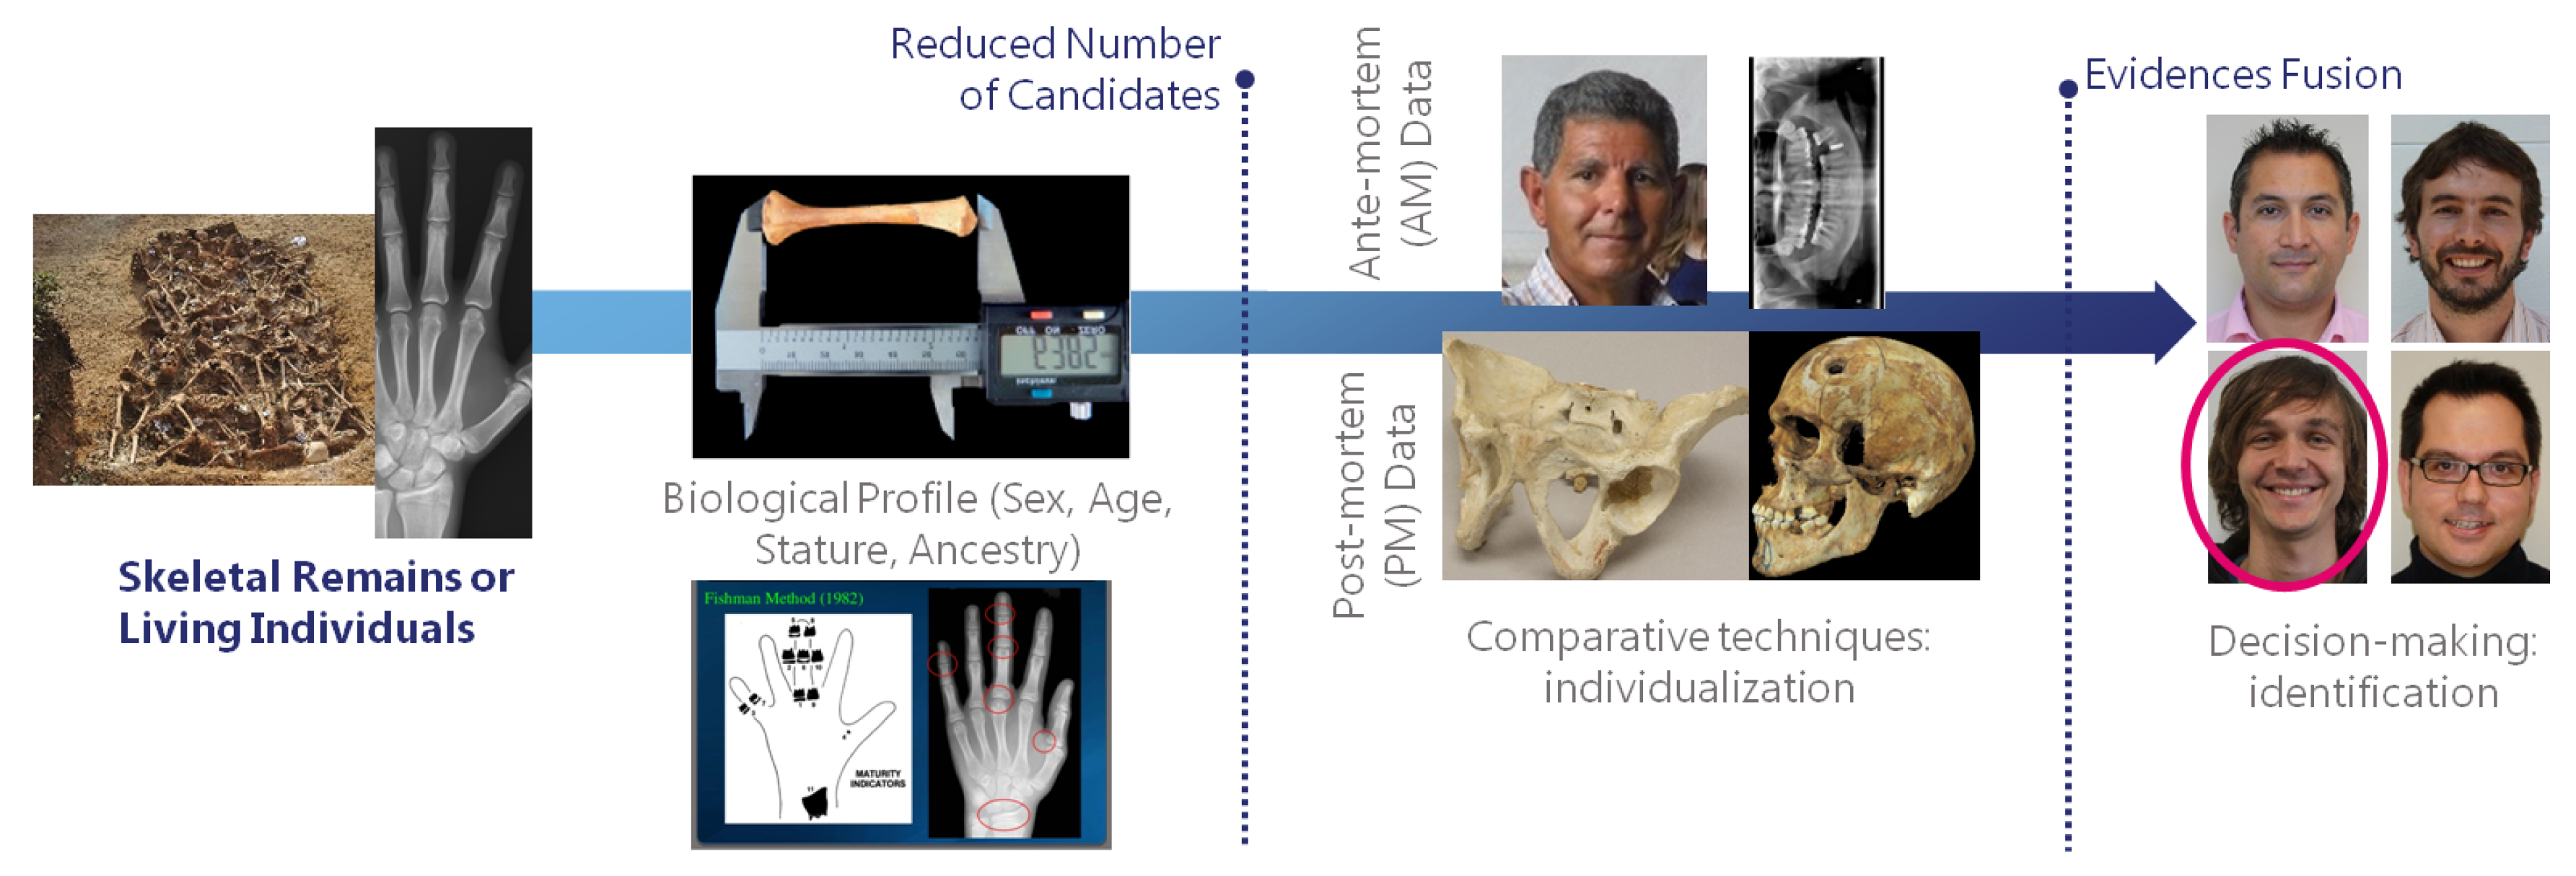
\includegraphics[width=1\linewidth]{figures/1_introduction/intro_1.png}
    \caption[Proceso general de identificación forense a partir de restos óseos o individuos vivos]{Proceso general de identificación forense a partir de restos óseos o individuos vivos mediante técnicas de análisis de imágenes biomédicas. A partir de los restos óseos o radiografías, se estima el perfil biológico (sexo, edad, estatura y ascendencia), lo cual permite reducir el número de posibles candidatos. Posteriormente, se realiza la comparación entre datos post-mortem y datos ante-mortem, utilizando técnicas comparativas como la superposición craneofacial o el análisis de estructuras dentales y esqueléticas. Finalmente, la fusión de evidencias conduce al proceso de toma de decisiones e identificación del individuo. Figura tomada de \cite{RefWorks:RefID:21-mesejo2020survey}.}
    \label{fig:intro_1}
\end{figure}

La estimación de la edad de la muerte es el campo más activo de la AF \cite{ubelaker_recent_2020} y que requiere por tanto un alto grado de automatización y fiabilidad. Para llevar a cabo dicha estimación, se examinan estructuras como las suturas craneales \cite{skullAF}, las costillas \cite{icscan1984age}, la cara auricular del ilion \cite{osborne_reconsidering_2004} y la sínfisis del pubis \cite{garvin_current_2012}, estos dos últimos localizados en la pelvis. En cada caso, se observa el grado de desgaste que presentan estos huesos en el momento del fallecimiento, lo cual permite aproximarse a la edad del individuo \cite{RefWorks:RefID:12-black2011forensic}.

La sínfisis del pubis es el hueso más utilizado para estimar la edad de un individuo ya fallecido, siendo la opción preferida por el 95\% de los antropólogos forenses \cite{garvin_current_2012}. El método predominante se fundamenta en el trabajo pionero de Thomas Wingate Todd \cite{RefWorks:RefID:19-todd1921age}, quien en 1921 documentó las transformaciones progresivas de la sínfisis del pubis con el envejecimiento, permitiendo estimar un rango aproximado de edad al momento del fallecimiento. Todd propuso un sistema de etapas de envejecimiento que ha sido revisado y perfeccionado en múltiples ocasiones, siendo la revisión de Suchey-Brooks \cite{RefWorks:RefID:20-brooks1990skeletal}, publicada en 1990, posiblemente la más reconocida de todas. Tanto el método original de Todd como la revisión de Suchey-Brooks se basan en el análisis de diferentes características de la sínfisis del pubis. En función del estado de cada una, asignan atributos categóricos que reflejan el grado de erosión ósea en distintas áreas, permitiendo así calcular un rango estimado de edad para el difunto. Dichas características varían según el método, en este TFM se utilizan las 9 características propuestas por Villar et al. \cite{villar2017first} y descritas en un atlas propuesto por \cite{irurita2025pubic} para el método de Todd, que se detallan en la Tabla \ref{table:themBones}, y en la Tabla \ref{themBomes:visualExample} se presenta un ejemplo visual de algunas.

\begin{table}[h]
    \centering
% \resizebox{\textwidth}{!}{%
\begin{tabular}{ccc}
    \hline
    \rowcolor[HTML]{D33333} 
    \multicolumn{1}{c|}{\cellcolor[HTML]{D33333}{\color[HTML]{FFFFFF} Característica}} & \multicolumn{2}{c}{\cellcolor[HTML]{D33333}{\color[HTML]{FFFFFF} Atributos}} \\ \hline
    \rowcolor[HTML]{FFCCC9} 
    \multicolumn{1}{|c}{\cellcolor[HTML]{FD6864}Crestas y Surcos} & Porosidad Regular & \multicolumn{1}{c|}{\cellcolor[HTML]{FFCCC9}Muy Definidas} \\ \cline{1-1}
    \multicolumn{1}{c|}{} & \cellcolor[HTML]{FFCCC9}Poco Profundas & \multicolumn{1}{c|}{\cellcolor[HTML]{FFCCC9}Restos de Surcos} \\ \cline{3-3} 
    \multicolumn{1}{c|}{} & \multicolumn{1}{c|}{\cellcolor[HTML]{FFCCC9}No hay surcos} &  \\ \hline
    \rowcolor[HTML]{FFCCC9} 
    \multicolumn{1}{|c}{\cellcolor[HTML]{FD6864}Porosidad Irregular} & No & \multicolumn{1}{c|}{\cellcolor[HTML]{FFCCC9}Mediana} \\ \cline{1-1} \cline{3-3} 
    \multicolumn{1}{c|}{} & \multicolumn{1}{c|}{\cellcolor[HTML]{FFCCC9}Si} &  \\ \hline
    \rowcolor[HTML]{FFCCC9} 
    \multicolumn{1}{|c}{\cellcolor[HTML]{FD6864}Borde Superior} & No Definido & \multicolumn{1}{c|}{\cellcolor[HTML]{FFCCC9}Definido} \\ \hline
    \rowcolor[HTML]{FFCCC9} 
    \multicolumn{1}{|c}{\cellcolor[HTML]{FD6864}Nódulo Óseo} & Ausente & \multicolumn{1}{c|}{\cellcolor[HTML]{FFCCC9}Presente} \\ \hline
    \rowcolor[HTML]{FFCCC9} 
    \multicolumn{1}{|c}{\cellcolor[HTML]{FD6864}Borde Inferior} & No Definido & \multicolumn{1}{c|}{\cellcolor[HTML]{FFCCC9}Definido} \\ \hline
    \rowcolor[HTML]{FFCCC9} 
    \multicolumn{1}{|c}{\cellcolor[HTML]{FD6864}Plataforma Dorsal} & Ausente & \multicolumn{1}{c|}{\cellcolor[HTML]{FFCCC9}En Formación} \\ \cline{1-1} \cline{3-3} 
    \multicolumn{1}{l|}{} & \multicolumn{1}{c|}{\cellcolor[HTML]{FFCCC9}Presente} & \multicolumn{1}{l}{} \\ \hline
    \rowcolor[HTML]{FFCCC9} 
    \multicolumn{1}{|c}{\cellcolor[HTML]{FD6864}Borde Dorsal} & Ausente & \multicolumn{1}{c|}{\cellcolor[HTML]{FFCCC9}En Formación} \\ \cline{1-1} \cline{3-3} 
    \multicolumn{1}{l|}{} & \multicolumn{1}{c|}{\cellcolor[HTML]{FFCCC9}Presente} & \multicolumn{1}{l}{} \\ \hline
    \rowcolor[HTML]{FFCCC9} 
    \multicolumn{1}{|c}{\cellcolor[HTML]{FD6864}Bisel Ventral} & Ausente & \multicolumn{1}{c|}{\cellcolor[HTML]{FFCCC9}En Formación} \\ \cline{1-1} \cline{3-3} 
    \multicolumn{1}{c|}{} & \multicolumn{1}{c|}{\cellcolor[HTML]{FFCCC9}Presente} &  \\ \hline
    \rowcolor[HTML]{FFCCC9} 
    \multicolumn{1}{|c}{\cellcolor[HTML]{FD6864}Borde Ventral} & Ausente & \multicolumn{1}{c|}{\cellcolor[HTML]{FFCCC9}En Formación} \\ \cline{1-1}
    \multicolumn{1}{c|}{} & \cellcolor[HTML]{FFCCC9}Formado, Sin Excrecencias & \multicolumn{1}{c|}{\cellcolor[HTML]{FFCCC9}Formado, Pocas Excrecencias} \\ \cline{3-3} 
    \multicolumn{1}{c|}{} & \multicolumn{1}{c|}{\cellcolor[HTML]{FFCCC9}Formado, Muchas Excrecencias} &  \\ \cline{2-2}
\end{tabular}%
% }
\caption[Método de Todd: Características y atributos para determinación de edad]{Características y atributos utilizados para la determinación de la edad según el método de Todd \cite{RefWorks:RefID:19-todd1921age} propuestos en Villar et al. \cite{villar2017first}.}
\label{table:themBones}
\end{table}

\begin{table}[htbp]
    \centering
    \begin{tabular}{|
    >{\columncolor[HTML]{D33333}}c |c|cc}
    \hline
    {\color[HTML]{FFFFFF} \textbf{Característica}} & \begin{tabular}[c]{@{}c@{}}Crestas y Surcos\end{tabular} & \multicolumn{1}{c|}{\begin{tabular}[c]{@{}c@{}}Porosidad  Irregular\end{tabular}} & \multicolumn{1}{c|}{\begin{tabular}[c]{@{}c@{}}Borde Superior\end{tabular}} \\ \hline
    {\color[HTML]{FFFFFF} \textbf{Atributo}} & Muy Definidos & \multicolumn{1}{c|}{Sí} & \multicolumn{1}{c|}{Definido} \\ \hline
    {\color[HTML]{FFFFFF} \textbf{Ejemplo}} & 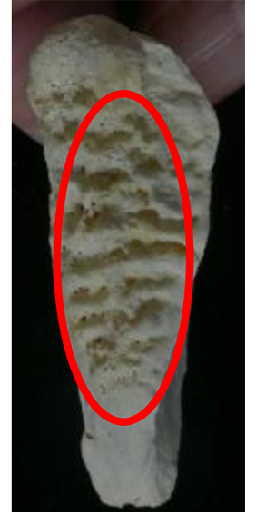
\includegraphics[align=c, width=0.2\linewidth]{figures/1_introduction/todd1.png} & \multicolumn{1}{c|}{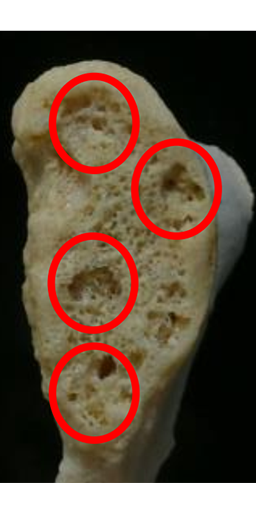
\includegraphics[align=c, width=0.2\linewidth]{figures/1_introduction/todd2.png}} & \multicolumn{1}{c|}{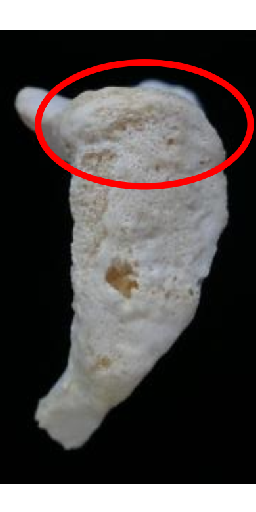
\includegraphics[align=c, width=0.2\linewidth]{figures/1_introduction/todd3.png}} \\ \hline
    {\color[HTML]{FFFFFF} \textbf{Característica}} & \begin{tabular}[c]{@{}c@{}}Nódulo Óseo\end{tabular} & \multicolumn{1}{c|}{\begin{tabular}[c]{@{}c@{}}Borde Inferior\end{tabular}} & \multicolumn{1}{c|}{\begin{tabular}[c]{@{}c@{}}Borde Dorsal\end{tabular}} \\ \hline
    {\color[HTML]{FFFFFF} \textbf{Atributo}} & Presente & \multicolumn{1}{c|}{Definido} & \multicolumn{1}{c|}{Definido} \\ \hline
    {\color[HTML]{FFFFFF} \textbf{Ejemplo}} & 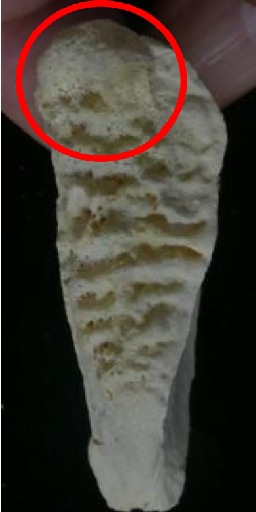
\includegraphics[align=c, width=0.2\linewidth]{figures/1_introduction/todd4.png} & \multicolumn{1}{c|}{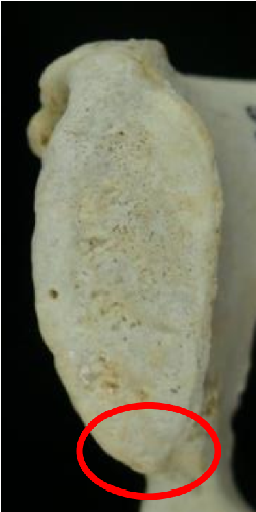
\includegraphics[align=c, width=0.2\linewidth]{figures/1_introduction/todd5.png}} & \multicolumn{1}{c|}{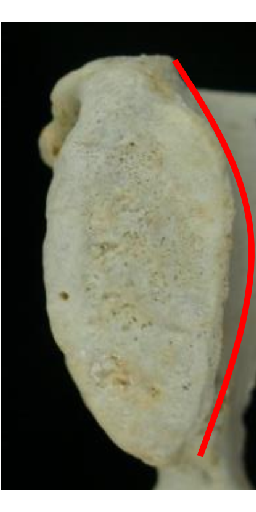
\includegraphics[align=c, width=0.2\linewidth]{figures/1_introduction/todd6.png}} \\ \hline
    {\color[HTML]{FFFFFF} \textbf{Característica}} & \begin{tabular}[c]{@{}c@{}}Plataforma Dorsal\end{tabular} & \multicolumn{1}{l}{} & \multicolumn{1}{l}{} \\ \cline{1-2}
    {\color[HTML]{FFFFFF} \textbf{Atributo}} & Presente & \multicolumn{1}{l}{} & \multicolumn{1}{l}{} \\ \cline{1-2}
    {\color[HTML]{FFFFFF} \textbf{Ejemplo}} & 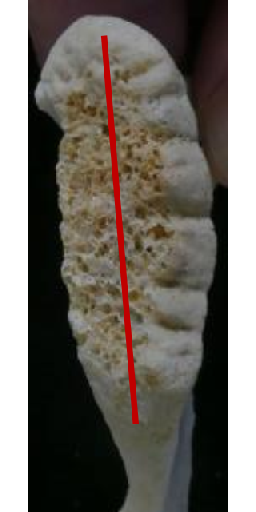
\includegraphics[align=c, width=0.2\linewidth]{figures/1_introduction/todd7.png} & \multicolumn{1}{l}{} & \multicolumn{1}{l}{} \\ \cline{1-2}
    \end{tabular}
    \caption[Método de Todd: Ejemplo visual de algunas características y atributos]{Ejemplos visuales de algunas de las características y atributos del método de Todd.}
    \label{themBomes:visualExample}
\end{table}

Es importante destacar que, al igual que en muchas otras tareas de la AF, la anotación de las características en las que se basan los métodos de estimación de la edad señalados depende en gran medida del criterio subjetivo del experto. Esto genera errores intra- e inter-experto \cite{irurita2025pubic}, ya que el uso de criterios subjetivos y descriptivos introduce limitaciones debido a las diversas interpretaciones entre evaluadores \cite{RefWorks:RefID:12-black2011forensic}. Tal situación disminuye la confiabilidad y validez de los resultados obtenidos, lo que finalmente reduce la credibilidad de los estudios forenses cuando se presentan como evidencia en un juicio (como se indicará más abajo cuando se mencione el estándar de Daubert). Esta problemática justifica la búsqueda de herramientas y metodologías que, al menos parcialmente, mitiguen dichas limitaciones. En este contexto, disciplinas como la inteligencia artificial (IA) \cite{russell_artificial_2021} y, en particular, el aprendizaje automático (\textit{Machine Learning}, ML) \cite{abu-mostafa_learning_2012, bishop_pattern_2019, murphy_probabilistic_2022, murphy_probabilistic_2023}, el aprendizaje profundo (\textit{Deep Learning}, DL) \cite{Goodfellow-et-al-2016, bishop_deep_2024, prince_understanding_2023} y la visión por computador (\textit{Computer Vision}, CV) \cite{torralba_foundations_2024, szeliski_computer_2022} pueden asistir, automatizar y acelerar las tareas forenses, reduciendo significativamente los sesgos y errores.

Considerando todo lo anterior, \textbf{el presente TFM se centra en la clasificación automática de las características morfológicas de la sínfisis del pubis para estimar la edad de la muerte a partir de modelos 3D mediante técnicas de IA.}

\section{Motivación}
En las últimas décadas los avances en IA, especialmente en ML y CV, han facilitado tanto la automatización de tareas repetitivas y tediosas como la superación del rendimiento humano en actividades complejas. En estos ámbitos, se han logrado avances significativos en tareas como la clasificación y segmentación de imágenes \cite{edozie_comprehensive_2025}, la detección de objetos en las mismas \cite{liu_deep_2020}, generación de imagen y vídeo \cite{wang_generative_2021} así como la reconstrucción de imágenes \cite{xie_review_2022}. Estas técnicas han sido ampliamente adoptadas en diversas disciplinas \cite{chai_deep_2021}, incluida la medicina, donde han proporcionado herramientas de gran utilidad para los profesionales del área \cite{esteva_deep_2021}.

No obstante, resulta sorprendente que, en la actualidad, la AF siga presentando un nivel relativamente bajo de sofisticación tecnológica \cite{RefWorks:RefID:21-mesejo2020survey}. En este contexto, una de las principales motivaciones de este trabajo es impulsar la modernización y automatización de la AF desde una perspectiva tecnológica, centrándose particularmente en la aplicación de técnicas avanzadas para la estimación de edad.

Además, como se mencionó previamente, la subjetividad inherente a la AF representa un desafío desde el punto de vista legal. En muchos casos, los análisis carecen de una base científica sólida según el criterio de Daubert \cite{noauthor_daubert_nodate}, el cual establece los requisitos para la admisibilidad del testimonio experto en un juicio. Según este criterio, un método es válido si: (1) los resultados son reproducibles y han sido verificados por terceros, (2) posee tasas de error conocidas y (3) es aceptado por la comunidad científica forense.

En este sentido, la aplicación de IA en AF puede contribuir significativamente a la reducción de la subjetividad en las identificaciones, minimizando errores humanos, y acelerando la realización de múltiples tareas, estructurando el conocimiento experto y facilitando la obtención de nuevos hallazgos. Esto, a su vez, fortalecería la base científica de los métodos utilizados en la disciplina, permitiendo que sean reproducibles y que se conozcan con precisión sus tasas de error, lo que favorecería su cumplimiento con el criterio de Daubert y su aceptación en el ámbito legal.

Si se analiza el contexto global de la identificación humana, se evidencia que la estimación del PB mediante técnicas de AF adquiere especial relevancia, puesto que otras herramientas de mayor precisión y sofisticación, como el análisis de ADN o la toma de huellas dactilares, presentan limitaciones significativas \cite{de_boer_role_2019, beauthier_mass_2009}. Por ejemplo, el análisis de ADN requiere una inversión elevada en recursos y tiempo, y al igual que la obtención de huellas dactilares, depende de la disponibilidad de datos tanto ante-mortem como post-mortem. Además, ambas técnicas se ven afectadas por el estado de los tejidos blandos, que son los más susceptibles a la descomposición natural o a daños provocados por quemaduras y exposición a agua o productos químicos, entre otros factores. En cambio, el tejido óseo, en general, demuestra una mayor resistencia y es frecuentemente lo único recuperable tras la completa descomposición de los tejidos blandos. Por ello, las técnicas basadas en AF son especialmente útiles en los siguientes escenarios:

\begin{itemize}
    \item Identificación masiva de víctimas de desastres naturales, accidentes o ataques terroristas.
    \item Identificación de víctimas de conflictos armados o actos de lesa humanidad, donde los restos pueden estar desmembrados, desfigurados y/o quemados.
    \item Procesamiento de fosas comunes en las que los restos óseos se han mezclado.
    \item Identificación de personas desaparecidas en contextos no relacionados con desastres o guerras, en los que las condiciones del cadáver han impedido la aplicación de otras técnicas \cite{byers_introduction_2016}.
\end{itemize}

Para dimensionar el desafío al que se enfrentan los antropólogos forenses, es relevante considerar que, únicamente en el año 2019, 20,000 personas perdieron la vida por causas vinculadas al terrorismo, con un promedio anual de 24,000 muertes en la última década atribuibles a este fenómeno \cite{owid_terrorism}. Asimismo, los desastres naturales ocasionan aproximadamente entre 40,000 y 50,000 muertes anuales \cite{owid_natural_disasters}. En el caso de Gaza, al momento de la redacción de este documento, se estima que entre 56,000 y 80,000 personas han sido asesinadas como resultado de los bombardeos, mientras que al menos 11,000 permanecen desaparecidas bajo los escombros, según datos del Ministerio de Salud y la ONU \cite{morales_56000_2025}. En España, aún se deben recuperar alrededor de 20,000 víctimas de la Guerra Civil, muchas de las cuales se hallan en fosas y cunetas, de modo que apenas un tercio de ellas podría ser identificada mediante análisis de ADN \cite{junquera_huellas_2022}.

Estos datos subrayan la necesidad de incorporar técnicas informáticas automatizadas en el ámbito de la AF, ya que permitirían una considerable optimización en términos de tiempo y recursos, facilitando la detección de las características determinantes para la estimación de la edad en situaciones en las que el número de individuos a identificar es elevado y otras técnicas no son aplicables.

\section{Objetivos}

Tras haber descrito el problema y su motivación, el objetivo principal de este TFM consiste en desarrollar y validar un modelo de aprendizaje profundo que, a partir de modelos 3D de la sínfisis púbica, permita extraer características morfológicas relevantes para la estimación de la edad en el momento de la muerte.

Cabe destacar que este trabajo se construye como una continuación directa del TFG desarrollado previamente por el propio autor \cite{lugli_tfg_2022}\footnote{Galardonado con el Premio a Mejor TFG del Grado de Ingeniería Informática por la E.T.S. de Ingenierías Informática y de Telecomunicación de la Universidad de Granada, 10 de mayo de 2023.}. En dicho trabajo preliminar se exploró un método que fue en ese momento el estado del arte para el procesamiento de los escaneos 3D de la sínfisis del pubis, donde solo se centró en la predicción de una de las nueve características morfológicas del método de Todd, concretamente el Nódulo Óseo. Se realizó con una cantidad mucho más restringida de datos y de capacidad de cómputo. Aun así se lograron resultados prometedores, siendo esta la razón de ser de este proyecto actual.

El presente TFM amplía sustancialmente dicho enfoque inicial, incorporando técnicas más actuales y sofisticadas de DL para datos 3D, así como procedimientos más avanzados para la obtención de la arquitectura e hiperparámetros de dichos modelos. Además, se aborda un volumen experimental considerablemente mayor y se incorpora el análisis del efecto de la resolución de las mallas sobre el rendimiento predictivo así como una visión a la interpretabilidad de los modelos obtenidos. Todo ello con el objetivo de avanzar hacia un sistema más robusto, reproducible y explicable para la clasificación automática de las características morfológicas utilizadas en la estimación de la edad de la muerte.

Este objetivo principal se desglosa en los siguientes objetivos parciales:

\begin{enumerate}
    \item Realizar un estudio exhaustivo de la literatura relativa a la estimación de edad a partir de restos óseos y al procesamiento de modelos 3D mediante redes neuronales profundas.
    \item Analizar y discutir los enfoques y modelos existentes, seleccionando de forma razonada los candidatos más prometedores para el problema abordado.
    \item Generar, entrenar y evaluar de forma extensiva múltiples arquitecturas de DL con el fin de identificar configuraciones óptimas que permitan predecir con precisión las nueve características morfológicas del método de Todd, tanto desde una perspectiva multiclase como multietiqueta.
\end{enumerate}

\section{Planificación del proyecto}

El presente trabajo consiste, en esencia, en el diseño e implementación de un software de carácter investigador. Para su planificación, es importante considerar que la asignatura del TFM está dotada con 12 créditos ECTS, lo que equivale a un total de 300 horas de trabajo, tomando como referencia que un crédito representa 25 horas.

Teniendo en cuenta que el autor compagina este proyecto con una actividad laboral a tiempo completo, se ha optado por una estimación conservadora que contempla la realización del TFM a lo largo de un curso académico completo, es decir, en un plazo aproximado de 40 semanas. Esto se traduce en una dedicación semanal de 7.5 horas, repartidas en sesiones de una hora y media diaria durante cinco días a la semana.

Dado que el proyecto cuenta con unos requisitos y objetivos bien definidos, no se prevén grandes desviaciones respecto a su desarrollo original. Por ello, se ha optado por emplear la metodología de desarrollo de software en cascada \cite{pressman2005software}, que organiza el proceso en fases secuenciales: análisis, diseño, codificación o desarrollo, pruebas y mantenimiento.

No obstante, es importante señalar que el modelo en cascada rara vez se aplica de forma estricta, ya que su estructura lineal impide retroceder a fases previas una vez completadas. Esto requeriría un conocimiento absoluto y estable de los requisitos desde el inicio, así como la ausencia de errores en etapas posteriores, condiciones poco realistas en la mayoría de proyectos de investigación. Por esta razón, se adopta una variante más flexible conocida como modelo en cascada con retroalimentación, que permite retornar a fases anteriores cuando sea necesario, ya sea para corregir errores, resolver ambigüedades o adaptar el diseño a cambios en los requisitos detectados durante el desarrollo.

Las fases del ciclo de vida del software se adaptaron al proyecto de la siguiente manera:

\begin{itemize}
\item \textbf{Análisis de Requisitos:} Esta fase incluyó las reuniones iniciales con los directores del TFM y los expertos en AF, quienes actuaron como usuarios finales del sistema. También se realizó una revisión bibliográfica exhaustiva, tanto en el ámbito de la AF como en su intersección con técnicas automáticas de IA. El objetivo fue establecer con precisión los objetivos del proyecto y delimitar su alcance.

\item \textbf{Diseño:} En esta etapa se investigaron y seleccionaron las técnicas más adecuadas para abordar el problema, incluyendo la elección de modelos, métricas y protocolos de validación experimental. Asimismo, se llevaron a cabo pruebas preliminares para verificar la viabilidad técnica de las distintas configuraciones y metodologías seleccionadas.

\item \textbf{Desarrollo:} Consistió en la adaptación del código base de las técnicas seleccionadas, así como en el desarrollo de funcionalidades adicionales. Se implementaron también herramientas de soporte en forma de \textit{scripts} para el preprocesado de los datos, así como para el cálculo automatizado de métricas y datos.

\item \textbf{Pruebas:} Esta fase se centró en la realización de experimentos sistemáticos sobre los modelos y configuraciones seleccionadas, con el objetivo de evaluar el rendimiento y extraer conclusiones sobre la efectividad de las soluciones propuestas.

\item \textbf{Informe:} En esta fase se procedió a la documentación de todo el proceso en el presente informe, detallando las motivaciones, fundamentos teóricos, metodología, resultados obtenidos, análisis y conclusiones del trabajo.
\end{itemize}

La planificación inicial del proyecto puede consultarse en la Tabla \ref{table:plan1}, en la cual se contempló un mes adicional como margen para posibles imprevistos o retrasos en la ejecución del trabajo. Se estimó un total de 307.5 horas totales para realizar el TFM.

\begin{table}[h]
\centering
\resizebox{\textwidth}{!}{%
\begin{tabular}{|c|c|ccccccccccccccccccccccc}
    \hline
    \rowcolor[HTML]{D33333} 
    \cellcolor[HTML]{D33333}{\color[HTML]{FFFFFF} } & \cellcolor[HTML]{D33333}{\color[HTML]{FFFFFF} } & \multicolumn{2}{c|}{\cellcolor[HTML]{D33333}{\color[HTML]{FFFFFF} \textbf{Septiembre}}} & \multicolumn{4}{c|}{\cellcolor[HTML]{D33333}{\color[HTML]{FFFFFF} \textbf{Octubre}}} & \multicolumn{4}{c|}{\cellcolor[HTML]{D33333}{\color[HTML]{FFFFFF} \textbf{Noviembre}}} & \multicolumn{5}{c|}{\cellcolor[HTML]{D33333}{\color[HTML]{FFFFFF} \textbf{Diciembre}}} & \multicolumn{4}{c|}{\cellcolor[HTML]{D33333}{\color[HTML]{FFFFFF} \textbf{Enero}}} & \multicolumn{4}{c|}{\cellcolor[HTML]{D33333}{\color[HTML]{FFFFFF} \textbf{Febrero}}} \\ \cline{3-25} 
    \rowcolor[HTML]{D33333} 
    \multirow{-2}{*}{\cellcolor[HTML]{D33333}{\color[HTML]{FFFFFF} \textbf{Tarea}}} & \multirow{-2}{*}{\cellcolor[HTML]{D33333}{\color[HTML]{FFFFFF} \textbf{\begin{tabular}[c]{@{}c@{}}Semanas – \\ Horas\end{tabular}}}} & \multicolumn{1}{c|}{\cellcolor[HTML]{D33333}{\color[HTML]{FFFFFF} \textbf{23}}} & \multicolumn{1}{c|}{\cellcolor[HTML]{D33333}{\color[HTML]{FFFFFF} \textbf{30}}} & \multicolumn{1}{c|}{\cellcolor[HTML]{D33333}{\color[HTML]{FFFFFF} \textbf{7}}} & \multicolumn{1}{c|}{\cellcolor[HTML]{D33333}{\color[HTML]{FFFFFF} \textbf{14}}} & \multicolumn{1}{c|}{\cellcolor[HTML]{D33333}{\color[HTML]{FFFFFF} \textbf{21}}} & \multicolumn{1}{c|}{\cellcolor[HTML]{D33333}{\color[HTML]{FFFFFF} \textbf{28}}} & \multicolumn{1}{c|}{\cellcolor[HTML]{D33333}{\color[HTML]{FFFFFF} \textbf{4}}} & \multicolumn{1}{c|}{\cellcolor[HTML]{D33333}{\color[HTML]{FFFFFF} \textbf{11}}} & \multicolumn{1}{c|}{\cellcolor[HTML]{D33333}{\color[HTML]{FFFFFF} \textbf{18}}} & \multicolumn{1}{c|}{\cellcolor[HTML]{D33333}{\color[HTML]{FFFFFF} \textbf{25}}} & \multicolumn{1}{c|}{\cellcolor[HTML]{D33333}{\color[HTML]{FFFFFF} \textbf{2}}} & \multicolumn{1}{c|}{\cellcolor[HTML]{D33333}{\color[HTML]{FFFFFF} \textbf{9}}} & \multicolumn{1}{c|}{\cellcolor[HTML]{D33333}{\color[HTML]{FFFFFF} \textbf{16}}} & \multicolumn{1}{c|}{\cellcolor[HTML]{D33333}{\color[HTML]{FFFFFF} \textbf{23}}} & \multicolumn{1}{c|}{\cellcolor[HTML]{D33333}{\color[HTML]{FFFFFF} \textbf{30}}} & \multicolumn{1}{c|}{\cellcolor[HTML]{D33333}{\color[HTML]{FFFFFF} \textbf{6}}} & \multicolumn{1}{c|}{\cellcolor[HTML]{D33333}{\color[HTML]{FFFFFF} \textbf{13}}} & \multicolumn{1}{c|}{\cellcolor[HTML]{D33333}{\color[HTML]{FFFFFF} \textbf{20}}} & \multicolumn{1}{c|}{\cellcolor[HTML]{D33333}{\color[HTML]{FFFFFF} \textbf{27}}} & \multicolumn{1}{c|}{\cellcolor[HTML]{D33333}{\color[HTML]{FFFFFF} \textbf{3}}} & \multicolumn{1}{c|}{\cellcolor[HTML]{D33333}{\color[HTML]{FFFFFF} \textbf{10}}} & \multicolumn{1}{c|}{\cellcolor[HTML]{D33333}{\color[HTML]{FFFFFF} \textbf{17}}} & \multicolumn{1}{c|}{\cellcolor[HTML]{D33333}{\color[HTML]{FFFFFF} \textbf{24}}} \\ \hline
    \textbf{\begin{tabular}[c]{@{}c@{}}Análisis \\ de Requisitos\end{tabular}} & 7 - 52.5 & \cellcolor[HTML]{FFCCC9} & \cellcolor[HTML]{FFCCC9} & \cellcolor[HTML]{FFCCC9} & \cellcolor[HTML]{FFCCC9} & \cellcolor[HTML]{FFCCC9} & \cellcolor[HTML]{FFCCC9} & \cellcolor[HTML]{FFCCC9} &  &  &  &  &  &  &  &  &  &  &  &  &  &  &  & \multicolumn{1}{c|}{} \\ \hline
    \textbf{Diseño} & 11 - 82.5 &  &  &  &  &  &  &  & \cellcolor[HTML]{FFCCC9} & \cellcolor[HTML]{FFCCC9} & \cellcolor[HTML]{FFCCC9} & \cellcolor[HTML]{FFCCC9} & \cellcolor[HTML]{FFCCC9} & \cellcolor[HTML]{FFCCC9} & \cellcolor[HTML]{FFCCC9} & \cellcolor[HTML]{FFCCC9} & \cellcolor[HTML]{FFCCC9} & \cellcolor[HTML]{FFCCC9} & \cellcolor[HTML]{FFCCC9} &  &  &  &  & \multicolumn{1}{c|}{} \\ \hline
    \textbf{Desarrollo} & 5 - 37.5 &  &  &  &  &  &  &  &  &  &  &  &  &  &  &  &  &  &  & \cellcolor[HTML]{FFCCC9} & \cellcolor[HTML]{FFCCC9} & \cellcolor[HTML]{FFCCC9} & \cellcolor[HTML]{FFCCC9} & \multicolumn{1}{c|}{\cellcolor[HTML]{FFCCC9}} \\ \hline
    \textbf{Pruebas} & 0 - 0 &  &  &  &  &  &  &  &  &  &  &  &  &  &  &  &  &  &  &  &  &  &  & \multicolumn{1}{c|}{} \\ \hline
    \textbf{Informe} & 0 - 0 &  &  &  &  &  &  &  &  &  &  &  &  &  &  &  &  &  &  &  &  &  &  & \multicolumn{1}{c|}{} \\ \hline
    \cellcolor[HTML]{D33333}{\color[HTML]{FFFFFF} } & \cellcolor[HTML]{D33333}{\color[HTML]{FFFFFF} } & \multicolumn{5}{c|}{\cellcolor[HTML]{D33333}{\color[HTML]{FFFFFF} \textbf{Marzo}}} & \multicolumn{4}{c|}{\cellcolor[HTML]{D33333}{\color[HTML]{FFFFFF} \textbf{Abril}}} & \multicolumn{4}{c|}{\cellcolor[HTML]{D33333}{\color[HTML]{FFFFFF} \textbf{Mayo}}} & \multicolumn{5}{c|}{\cellcolor[HTML]{D33333}{\color[HTML]{FFFFFF} \textbf{Junio}}} & \multicolumn{4}{c|}{\cellcolor[HTML]{D33333}{\color[HTML]{FFFFFF} \textbf{Julio}}} & \textbf{} \\ \cline{3-24}
    \multirow{-2}{*}{\cellcolor[HTML]{D33333}{\color[HTML]{FFFFFF} \textbf{Tarea}}} & \multirow{-2}{*}{\cellcolor[HTML]{D33333}{\color[HTML]{FFFFFF} \textbf{\begin{tabular}[c]{@{}c@{}}Semanas – \\ Horas\end{tabular}}}} & \multicolumn{1}{c|}{\cellcolor[HTML]{D33333}{\color[HTML]{FFFFFF} \textbf{3}}} & \multicolumn{1}{c|}{\cellcolor[HTML]{D33333}{\color[HTML]{FFFFFF} \textbf{10}}} & \multicolumn{1}{c|}{\cellcolor[HTML]{D33333}{\color[HTML]{FFFFFF} \textbf{17}}} & \multicolumn{1}{c|}{\cellcolor[HTML]{D33333}{\color[HTML]{FFFFFF} \textbf{24}}} & \multicolumn{1}{c|}{\cellcolor[HTML]{D33333}{\color[HTML]{FFFFFF} \textbf{31}}} & \multicolumn{1}{c|}{\cellcolor[HTML]{D33333}{\color[HTML]{FFFFFF} \textbf{7}}} & \multicolumn{1}{c|}{\cellcolor[HTML]{D33333}{\color[HTML]{FFFFFF} \textbf{14}}} & \multicolumn{1}{c|}{\cellcolor[HTML]{D33333}{\color[HTML]{FFFFFF} \textbf{21}}} & \multicolumn{1}{c|}{\cellcolor[HTML]{D33333}{\color[HTML]{FFFFFF} \textbf{28}}} & \multicolumn{1}{c|}{\cellcolor[HTML]{D33333}{\color[HTML]{FFFFFF} \textbf{5}}} & \multicolumn{1}{c|}{\cellcolor[HTML]{D33333}{\color[HTML]{FFFFFF} \textbf{12}}} & \multicolumn{1}{c|}{\cellcolor[HTML]{D33333}{\color[HTML]{FFFFFF} \textbf{19}}} & \multicolumn{1}{c|}{\cellcolor[HTML]{D33333}{\color[HTML]{FFFFFF} \textbf{26}}} & \multicolumn{1}{c|}{\cellcolor[HTML]{D33333}{\color[HTML]{FFFFFF} \textbf{2}}} & \multicolumn{1}{c|}{\cellcolor[HTML]{D33333}{\color[HTML]{FFFFFF} \textbf{9}}} & \multicolumn{1}{c|}{\cellcolor[HTML]{D33333}{\color[HTML]{FFFFFF} \textbf{16}}} & \multicolumn{1}{c|}{\cellcolor[HTML]{D33333}{\color[HTML]{FFFFFF} \textbf{23}}} & \multicolumn{1}{c|}{\cellcolor[HTML]{D33333}{\color[HTML]{FFFFFF} \textbf{30}}} & \multicolumn{1}{c|}{\cellcolor[HTML]{D33333}{\color[HTML]{FFFFFF} \textbf{7}}} & \multicolumn{1}{c|}{\cellcolor[HTML]{D33333}{\color[HTML]{FFFFFF} \textbf{14}}} & \multicolumn{1}{c|}{\cellcolor[HTML]{D33333}{\color[HTML]{FFFFFF} \textbf{21}}} & \multicolumn{1}{c|}{\cellcolor[HTML]{D33333}{\color[HTML]{FFFFFF} \textbf{28}}} & \textbf{} \\ \cline{1-24}
    \textbf{\begin{tabular}[c]{@{}c@{}}Análisis \\ de Requisitos\end{tabular}} & 0 - 0 &  &  &  &  &  &  &  &  &  &  &  &  &  &  &  &  &  &  &  &  &  & \multicolumn{1}{c|}{} &  \\ \cline{1-24}
    \textbf{Diseño} & 0 - 0 &  &  &  &  &  &  &  &  &  &  &  &  &  &  &  &  &  &  &  &  &  & \multicolumn{1}{c|}{} &  \\ \cline{1-24}
    \textbf{Desarrollo} & 4 - 30 & \cellcolor[HTML]{FFCCC9} & \cellcolor[HTML]{FFCCC9} & \cellcolor[HTML]{FFCCC9} & \cellcolor[HTML]{FFCCC9} &  &  &  &  &  &  &  &  &  &  &  &  &  &  &  &  &  & \multicolumn{1}{c|}{} &  \\ \cline{1-24}
    \textbf{Pruebas} & 10 - 75 &  &  &  &  & \cellcolor[HTML]{FFCCC9} & \cellcolor[HTML]{FFCCC9} & \cellcolor[HTML]{FFCCC9} & \cellcolor[HTML]{FFCCC9} & \cellcolor[HTML]{FFCCC9} & \cellcolor[HTML]{FFCCC9} & \cellcolor[HTML]{FFCCC9} & \cellcolor[HTML]{FFCCC9} & \cellcolor[HTML]{FFCCC9} & \cellcolor[HTML]{FFCCC9} &  &  &  &  &  &  &  & \multicolumn{1}{c|}{} &  \\ \cline{1-24}
    \textbf{Informe} & 4 - 30 & \multicolumn{1}{l}{} & \multicolumn{1}{l}{} & \multicolumn{1}{l}{} & \multicolumn{1}{l}{} & \multicolumn{1}{l}{} & \multicolumn{1}{l}{} & \multicolumn{1}{l}{} & \multicolumn{1}{l}{} & \multicolumn{1}{l}{} & \multicolumn{1}{l}{} & \multicolumn{1}{l}{} & \multicolumn{1}{l}{} & \multicolumn{1}{l}{} & \multicolumn{1}{l}{} & \multicolumn{1}{l}{\cellcolor[HTML]{FFCCC9}} & \multicolumn{1}{l}{\cellcolor[HTML]{FFCCC9}} & \multicolumn{1}{l}{\cellcolor[HTML]{FFCCC9}} & \multicolumn{1}{l}{\cellcolor[HTML]{FFCCC9}} & \multicolumn{1}{l}{} & \multicolumn{1}{l}{} & \multicolumn{1}{l}{} & \multicolumn{1}{l|}{} & \multicolumn{1}{l}{} \\ \cline{1-24}
    \end{tabular}%
}
\caption[Planificación temporal inicial del proyecto]{Planificación temporal inicial del proyecto, considerándose el curso 2024-2025 para la realización del trabajo, más el mes de julio por posibles imprevistos o retrasos. Se estimó un esfuerzo total de 307.5 horas.}
\label{table:plan1}
\end{table}

Se realizó una planificación inicial con plazos deliberadamente relajados, teniendo en cuenta la situación laboral del autor. No obstante, dicha planificación experimentó modificaciones debido a diversas circunstancias. En primer lugar, el preprocesado de los datos resultó ser más laborioso de lo previsto, ya que fue necesario realizar múltiples experimentos para verificar la viabilidad y compatibilidad de los datos con el método seleccionado. Además, la alta complejidad y nivel de detalle de las mallas requirió un procesado más lento de las mismas para obtener un formato consistente y adecuado para el modelo de DL, lo que impactó significativamente en la duración de la fase de desarrollo.

Asimismo, la fase de pruebas se extendió más de lo previsto, ya que algunas versiones de los modelos de DL requerían tiempos de procesamiento considerablemente mayores debido a su alta complejidad, así como por errores esporádicos y difíciles de reproducir que surgían durante las ejecuciones. A esto se sumó la disponibilidad limitada del hardware necesario. Por otro lado, las fases de análisis de requisitos y diseño resultaron más breves, dado que se partía del trabajo desarrollado previamente en el TFG, lo que proporcionó una base sólida. Todos estos factores llevaron a una modificación de la planificación inicial, la cual se refleja en la Tabla \ref{table:plan2}. Se observa que se han utilizado un total de aproximadamente 337.5 horas para la realización del TFM.

\begin{table}[h]
\resizebox{\textwidth}{!}{%
\begin{tabular}{|c|c|ccccccccccccccccccccccc}
    \hline
    \rowcolor[HTML]{D33333} 
    \cellcolor[HTML]{D33333}{\color[HTML]{FFFFFF} } & \cellcolor[HTML]{D33333}{\color[HTML]{FFFFFF} } & \multicolumn{2}{c|}{\cellcolor[HTML]{D33333}{\color[HTML]{FFFFFF} \textbf{Septiembre}}} & \multicolumn{4}{c|}{\cellcolor[HTML]{D33333}{\color[HTML]{FFFFFF} \textbf{Octubre}}} & \multicolumn{4}{c|}{\cellcolor[HTML]{D33333}{\color[HTML]{FFFFFF} \textbf{Noviembre}}} & \multicolumn{5}{c|}{\cellcolor[HTML]{D33333}{\color[HTML]{FFFFFF} \textbf{Diciembre}}} & \multicolumn{4}{c|}{\cellcolor[HTML]{D33333}{\color[HTML]{FFFFFF} \textbf{Enero}}} & \multicolumn{4}{c|}{\cellcolor[HTML]{D33333}{\color[HTML]{FFFFFF} \textbf{Febrero}}} \\ \cline{3-25} 
    \rowcolor[HTML]{D33333} 
    \multirow{-2}{*}{\cellcolor[HTML]{D33333}{\color[HTML]{FFFFFF} \textbf{Tarea}}} & \multirow{-2}{*}{\cellcolor[HTML]{D33333}{\color[HTML]{FFFFFF} \textbf{\begin{tabular}[c]{@{}c@{}}Semanas – \\ Horas\end{tabular}}}} & \multicolumn{1}{c|}{\cellcolor[HTML]{D33333}{\color[HTML]{FFFFFF} \textbf{23}}} & \multicolumn{1}{c|}{\cellcolor[HTML]{D33333}{\color[HTML]{FFFFFF} \textbf{30}}} & \multicolumn{1}{c|}{\cellcolor[HTML]{D33333}{\color[HTML]{FFFFFF} \textbf{7}}} & \multicolumn{1}{c|}{\cellcolor[HTML]{D33333}{\color[HTML]{FFFFFF} \textbf{14}}} & \multicolumn{1}{c|}{\cellcolor[HTML]{D33333}{\color[HTML]{FFFFFF} \textbf{21}}} & \multicolumn{1}{c|}{\cellcolor[HTML]{D33333}{\color[HTML]{FFFFFF} \textbf{28}}} & \multicolumn{1}{c|}{\cellcolor[HTML]{D33333}{\color[HTML]{FFFFFF} \textbf{4}}} & \multicolumn{1}{c|}{\cellcolor[HTML]{D33333}{\color[HTML]{FFFFFF} \textbf{11}}} & \multicolumn{1}{c|}{\cellcolor[HTML]{D33333}{\color[HTML]{FFFFFF} \textbf{18}}} & \multicolumn{1}{c|}{\cellcolor[HTML]{D33333}{\color[HTML]{FFFFFF} \textbf{25}}} & \multicolumn{1}{c|}{\cellcolor[HTML]{D33333}{\color[HTML]{FFFFFF} \textbf{2}}} & \multicolumn{1}{c|}{\cellcolor[HTML]{D33333}{\color[HTML]{FFFFFF} \textbf{9}}} & \multicolumn{1}{c|}{\cellcolor[HTML]{D33333}{\color[HTML]{FFFFFF} \textbf{16}}} & \multicolumn{1}{c|}{\cellcolor[HTML]{D33333}{\color[HTML]{FFFFFF} \textbf{23}}} & \multicolumn{1}{c|}{\cellcolor[HTML]{D33333}{\color[HTML]{FFFFFF} \textbf{30}}} & \multicolumn{1}{c|}{\cellcolor[HTML]{D33333}{\color[HTML]{FFFFFF} \textbf{6}}} & \multicolumn{1}{c|}{\cellcolor[HTML]{D33333}{\color[HTML]{FFFFFF} \textbf{13}}} & \multicolumn{1}{c|}{\cellcolor[HTML]{D33333}{\color[HTML]{FFFFFF} \textbf{20}}} & \multicolumn{1}{c|}{\cellcolor[HTML]{D33333}{\color[HTML]{FFFFFF} \textbf{27}}} & \multicolumn{1}{c|}{\cellcolor[HTML]{D33333}{\color[HTML]{FFFFFF} \textbf{3}}} & \multicolumn{1}{c|}{\cellcolor[HTML]{D33333}{\color[HTML]{FFFFFF} \textbf{10}}} & \multicolumn{1}{c|}{\cellcolor[HTML]{D33333}{\color[HTML]{FFFFFF} \textbf{17}}} & \multicolumn{1}{c|}{\cellcolor[HTML]{D33333}{\color[HTML]{FFFFFF} \textbf{24}}} \\ \hline
    \textbf{\begin{tabular}[c]{@{}c@{}}Análisis \\ de Requisitos\end{tabular}} & 4 - 30 & \cellcolor[HTML]{FFCCC9} & \cellcolor[HTML]{FFCCC9} & \cellcolor[HTML]{FFCCC9} & \cellcolor[HTML]{FFCCC9} &  &  &  &  &  &  &  &  &  &  &  &  &  &  &  &  &  &  & \multicolumn{1}{c|}{} \\ \hline
    \textbf{Diseño} & 7 - 52.5 &  &  &  &  & \cellcolor[HTML]{FFCCC9} & \cellcolor[HTML]{FFCCC9} & \cellcolor[HTML]{FFCCC9} & \cellcolor[HTML]{FFCCC9} & \cellcolor[HTML]{FFCCC9} & \cellcolor[HTML]{FFCCC9} & \cellcolor[HTML]{FFCCC9} &  &  &  &  &  &  &  &  &  &  &  & \multicolumn{1}{c|}{} \\ \hline
    \textbf{Desarrollo} & 12 - 90 &  &  &  &  &  &  &  &  &  &  &  & \cellcolor[HTML]{FFCCC9} & \cellcolor[HTML]{FFCCC9} & \cellcolor[HTML]{FFCCC9} & \cellcolor[HTML]{FFCCC9} & \cellcolor[HTML]{FFCCC9} & \cellcolor[HTML]{FFCCC9} & \cellcolor[HTML]{FFCCC9} & \cellcolor[HTML]{FFCCC9} & \cellcolor[HTML]{FFCCC9} & \cellcolor[HTML]{FFCCC9} & \cellcolor[HTML]{FFCCC9} & \multicolumn{1}{c|}{\cellcolor[HTML]{FFCCC9}} \\ \hline
    \textbf{Pruebas} & 0 - 0 &  &  &  &  &  &  &  &  &  &  &  &  &  &  &  &  &  &  &  &  &  &  & \multicolumn{1}{c|}{} \\ \hline
    \textbf{Informe} & 0 - 0 &  &  &  &  &  &  &  &  &  &  &  &  &  &  &  &  &  &  &  &  &  &  & \multicolumn{1}{c|}{} \\ \hline
    \cellcolor[HTML]{D33333}{\color[HTML]{FFFFFF} } & \cellcolor[HTML]{D33333}{\color[HTML]{FFFFFF} } & \multicolumn{5}{c|}{\cellcolor[HTML]{D33333}{\color[HTML]{FFFFFF} \textbf{Marzo}}} & \multicolumn{4}{c|}{\cellcolor[HTML]{D33333}{\color[HTML]{FFFFFF} \textbf{Abril}}} & \multicolumn{4}{c|}{\cellcolor[HTML]{D33333}{\color[HTML]{FFFFFF} \textbf{Mayo}}} & \multicolumn{5}{c|}{\cellcolor[HTML]{D33333}{\color[HTML]{FFFFFF} \textbf{Junio}}} & \multicolumn{4}{c|}{\cellcolor[HTML]{D33333}{\color[HTML]{FFFFFF} \textbf{Julio}}} & \textbf{} \\ \cline{3-24}
    \multirow{-2}{*}{\cellcolor[HTML]{D33333}{\color[HTML]{FFFFFF} \textbf{Tarea}}} & \multirow{-2}{*}{\cellcolor[HTML]{D33333}{\color[HTML]{FFFFFF} \textbf{\begin{tabular}[c]{@{}c@{}}Semanas – \\ Horas\end{tabular}}}} & \multicolumn{1}{c|}{\cellcolor[HTML]{D33333}{\color[HTML]{FFFFFF} \textbf{3}}} & \multicolumn{1}{c|}{\cellcolor[HTML]{D33333}{\color[HTML]{FFFFFF} \textbf{10}}} & \multicolumn{1}{c|}{\cellcolor[HTML]{D33333}{\color[HTML]{FFFFFF} \textbf{17}}} & \multicolumn{1}{c|}{\cellcolor[HTML]{D33333}{\color[HTML]{FFFFFF} \textbf{24}}} & \multicolumn{1}{c|}{\cellcolor[HTML]{D33333}{\color[HTML]{FFFFFF} \textbf{31}}} & \multicolumn{1}{c|}{\cellcolor[HTML]{D33333}{\color[HTML]{FFFFFF} \textbf{7}}} & \multicolumn{1}{c|}{\cellcolor[HTML]{D33333}{\color[HTML]{FFFFFF} \textbf{14}}} & \multicolumn{1}{c|}{\cellcolor[HTML]{D33333}{\color[HTML]{FFFFFF} \textbf{21}}} & \multicolumn{1}{c|}{\cellcolor[HTML]{D33333}{\color[HTML]{FFFFFF} \textbf{28}}} & \multicolumn{1}{c|}{\cellcolor[HTML]{D33333}{\color[HTML]{FFFFFF} \textbf{5}}} & \multicolumn{1}{c|}{\cellcolor[HTML]{D33333}{\color[HTML]{FFFFFF} \textbf{12}}} & \multicolumn{1}{c|}{\cellcolor[HTML]{D33333}{\color[HTML]{FFFFFF} \textbf{19}}} & \multicolumn{1}{c|}{\cellcolor[HTML]{D33333}{\color[HTML]{FFFFFF} \textbf{26}}} & \multicolumn{1}{c|}{\cellcolor[HTML]{D33333}{\color[HTML]{FFFFFF} \textbf{2}}} & \multicolumn{1}{c|}{\cellcolor[HTML]{D33333}{\color[HTML]{FFFFFF} \textbf{9}}} & \multicolumn{1}{c|}{\cellcolor[HTML]{D33333}{\color[HTML]{FFFFFF} \textbf{16}}} & \multicolumn{1}{c|}{\cellcolor[HTML]{D33333}{\color[HTML]{FFFFFF} \textbf{23}}} & \multicolumn{1}{c|}{\cellcolor[HTML]{D33333}{\color[HTML]{FFFFFF} \textbf{30}}} & \multicolumn{1}{c|}{\cellcolor[HTML]{D33333}{\color[HTML]{FFFFFF} \textbf{7}}} & \multicolumn{1}{c|}{\cellcolor[HTML]{D33333}{\color[HTML]{FFFFFF} \textbf{14}}} & \multicolumn{1}{c|}{\cellcolor[HTML]{D33333}{\color[HTML]{FFFFFF} \textbf{21}}} & \multicolumn{1}{c|}{\cellcolor[HTML]{D33333}{\color[HTML]{FFFFFF} \textbf{28}}} & \textbf{} \\ \cline{1-24}
    \textbf{\begin{tabular}[c]{@{}c@{}}Análisis \\ de Requisitos\end{tabular}} & 0 - 0 &  &  &  &  &  &  &  &  &  &  &  &  &  &  &  &  &  &  &  &  &  & \multicolumn{1}{c|}{} &  \\ \cline{1-24}
    \textbf{Diseño} & 0 - 0 &  &  &  &  &  &  &  &  &  &  &  &  &  &  &  &  &  &  &  &  &  & \multicolumn{1}{c|}{} &  \\ \cline{1-24}
    \textbf{Desarrollo} & 3 - 22.5 & \cellcolor[HTML]{FFCCC9} &  & \cellcolor[HTML]{FFCCC9} &  & \cellcolor[HTML]{FFCCC9} &  &  &  &  &  &  &  &  &  &  &  &  &  &  &  &  & \multicolumn{1}{c|}{} &  \\ \cline{1-24}
    \textbf{Pruebas} & 10 - 75 &  & \cellcolor[HTML]{FFCCC9} &  & \cellcolor[HTML]{FFCCC9} &  & \cellcolor[HTML]{FFCCC9} & \cellcolor[HTML]{FFCCC9} & \cellcolor[HTML]{FFCCC9} & \cellcolor[HTML]{FFCCC9} & \cellcolor[HTML]{FFCCC9} & \cellcolor[HTML]{FFCCC9} & \cellcolor[HTML]{FFCCC9} & \cellcolor[HTML]{FFCCC9} &  &  &  &  &  &  &  &  & \multicolumn{1}{c|}{} &  \\ \cline{1-24}
    \textbf{Informe} & 9 - 67.5 &  &  &  &  &  &  &  &  &  &  &  &  &  & \cellcolor[HTML]{FFCCC9} & \cellcolor[HTML]{FFCCC9} & \cellcolor[HTML]{FFCCC9} & \cellcolor[HTML]{FFCCC9} & \cellcolor[HTML]{FFCCC9} & \cellcolor[HTML]{FFCCC9} & \cellcolor[HTML]{FFCCC9} & \cellcolor[HTML]{FFCCC9} & \multicolumn{1}{c|}{\cellcolor[HTML]{FFCCC9}} &  \\ \cline{1-24}
\end{tabular}%
}
\caption[Planificación temporal final del proyecto]{Planificación temporal final del proyecto, considerándose las modificaciones de los plazos debido a diversos factores. Se han utilizado un total de aproximadamente 337.5 horas en la realización del TFM}
\label{table:plan2}
\end{table}

Para la estimación del coste total del proyecto, se ha considerado un salario de 35\officialeuro/hora, correspondiente al perfil de un responsable de I+D en una empresa tecnológica o un investigador senior. Además, se han incluido los costes materiales, entre los que destacan: el precio del portátil empleado para el desarrollo del TFM, dispositivos de almacenamiento masivo, el uso de un servidor con GPU de altas prestaciones, y otros gastos misceláneos. El desglose completo puede consultarse en la Tabla \ref{table:money}, donde se estima el coste total del proyecto ronda los 19,550.00\officialeuro.

En particular, el servidor GPU se ha valorado en 15,000\officialeuro, asumiendo una amortización a dos años. Esto supone un coste diario de 20.55\officialeuro, lo que se traduce en 6,391.05\officialeuro\space durante el periodo estimado de duración del proyecto.

\begin{table}[h]
    \centering
    \begin{tabular}{ll}
        \hline
        \multicolumn{1}{|l|}{\cellcolor[HTML]{D33333}{\color[HTML]{FFFFFF} \textbf{Fecha inicio}}} & \multicolumn{1}{l|}{23/09/2024} \\ \hline
        \multicolumn{1}{|l|}{\cellcolor[HTML]{D33333}{\color[HTML]{FFFFFF} \textbf{Fecha fin}}} & \multicolumn{1}{l|}{31/07/2025} \\ \hline
        \multicolumn{1}{|l|}{\cellcolor[HTML]{D33333}{\color[HTML]{FFFFFF} \textbf{Duración}}} & \multicolumn{1}{l|}{311 días, 223 laborables} \\ \hline
         &  \\ \hline
        \rowcolor[HTML]{D33333} 
        \multicolumn{1}{|l|}{\cellcolor[HTML]{D33333}{\color[HTML]{FFFFFF} \textbf{Item}}} & \multicolumn{1}{l|}{\cellcolor[HTML]{D33333}{\color[HTML]{FFFFFF} \textbf{Costo}}} \\ \hline
        \multicolumn{1}{|l|}{Salario} & \multicolumn{1}{l|}{11,812.50\officialeuro} \\ \hline
        \multicolumn{1}{|l|}{Portátil} & \multicolumn{1}{l|}{800.00\officialeuro} \\ \hline
        \multicolumn{1}{|l|}{Servidor GPU} & \multicolumn{1}{l|}{6,391.05\officialeuro} \\ \hline
        \multicolumn{1}{|l|}{Almacenamiento} & \multicolumn{1}{l|}{150.00\officialeuro} \\ \hline
        \multicolumn{1}{|l|}{Otros} & \multicolumn{1}{l|}{400.00\officialeuro} \\ \hline
        \rowcolor[HTML]{FFCCC9} 
        \multicolumn{1}{|r|}{\cellcolor[HTML]{FFCCC9}Total} & \multicolumn{1}{l|}{\cellcolor[HTML]{FFCCC9}19,553.55\officialeuro} \\ \hline
    \end{tabular}
\caption{Estimación de coste del proyecto}
\label{table:money}
\end{table}


    % Fundamentos teóricos 
    \chapter{Fundamentos Teóricos}
Este capítulo tiene como objetivo introducir y explicar los fundamentos teóricos en los que se basan los métodos empleados en el trabajo, así como de su relevancia para la resolución del problema planteado.

\section{Aprendizaje Automático}
El Aprendizaje Automático, o \textit{Machine Learning} (ML) \cite{abu-mostafa_learning_2012, mitchell_introduction_1997, 6284961}, es una rama de la Inteligencia Artificial (IA) que se enfoca en el desarrollo de programas informáticos para resolver tareas complejas donde no existe una solución analítica directa. Es decir, no es posible describir un algoritmo que, dados los datos de entrada, los transforme en los datos de salida esperados. En estos casos, a menudo se carece de un conocimiento detallado y completo del problema, lo que puede intentarse compensar mediante el uso de datos relacionados. Estos datos pueden emplearse para obtener una solución empírica, donde el sistema "aprende" de ellos. A partir de los datos, se extraen patrones o reglas que permiten construir un algoritmo aproximado, conocido como modelo, capaz de resolver la tarea incluso cuando se enfrenta a datos no vistos previamente. Formalmente, se puede definir que un programa aprende de la experiencia $E$ en relación con una clase de tareas $T$ y una métrica de rendimiento $P$ si su rendimiento en las tareas $T$, medido por $P$, mejora con la experiencia $E$. Este aprendizaje se clasifica en dos grandes grupos: supervisado y no supervisado. En el aprendizaje supervisado, se dispone tanto de los datos de entrada como de las salidas correctas correspondientes, mientras que en el aprendizaje no supervisado solo se tienen los datos de entrada y se espera que el programa identifique patrones dentro de estos.

En términos generales, es factible aplicar ML en problemas que cumplen con alguna de las siguientes condiciones: (a) cuando se dispone de extensas bases de datos que permiten extraer patrones intrínsecos, lo que se conoce como minería de datos o \textit{data mining} \cite{alma991006986149704990}; (b) en aquellos problemas cuyos dominios no están bien definidos o en los que resulta difícil para un humano describirlos de manera precisa para desarrollar un algoritmo, como ocurre en tareas de detección de objetos en imágenes; y (c) en dominios en los que el sistema debe adaptarse de forma dinámica a condiciones cambiantes \cite{mitchell_introduction_1997}.

En el aprendizaje supervisado se distinguen dos tareas fundamentales: la clasificación y la regresión, cuya principal diferencia radica en la naturaleza de la variable de salida. En las tareas de clasificación, cada ejemplo de entrada se asigna a una categoría discreta. Esto implica que el modelo debe aprender a identificar y etiquetar cada muestra dentro de un conjunto finito de clases. Por otro lado, en las tareas de regresión el objetivo es predecir un valor numérico continuo. En este caso, la salida del modelo puede tomar cualquier valor dentro de un rango determinado.

A partir de las descripciones previas, se puede concluir que es viable aplicar técnicas de ML al problema en cuestión. En este caso, se dispone de datos de entrada, que corresponden a los huesos de la sínfisis del pubis, y de datos de salida, representados por los atributos de cada hueso clasificados según las nueve categorías del método de Todd. Además, aunque los antropólogos forenses poseen el conocimiento experto necesario para identificar estos patrones, dicho conocimiento no puede expresarse de manera analítica. Por ello, el problema se enmarca dentro del aprendizaje supervisado, siendo específicamente un problema de clasificación, ya que es necesario asignar a cada hueso los atributos correspondientes a las categorías establecidas por el método de Todd.

\section{Aprendizaje Profundo}
\label{section:DL}
El aprendizaje profundo (\textit{Deep Learning}, DL) \cite{Goodfellow-et-al-2016, lecun_deep_2015, schmidhuber_deep_2015} es una subdisciplina de ML en la que el modelo se encarga de aprender y extraer de manera automática las características relevantes a partir de los datos del problema. Esta aproximación contrasta con otras técnicas de ML en las que las características son diseñadas manualmente o \textit{handcrafted} por expertos que utilizan su conocimiento específico del dominio. Se ha demostrado que, para problemas de alta complejidad, las características extraídas de forma automática tienden a ser más efectivas y eficientes en comparación con aquellas obtenidas manualmente.

El modelo predominante en el ámbito del DL es la red neuronal artificial (\textit{Artificial Neural Network}, ANN) \cite{bishop_ANN, ripley_ANN}, compuesta por nodos de procesamiento, denominados \say{neuronas}{\interfootnotelinepenalty=10000 \footnote{Aunque su denominación es bioinspirada en la corteza visual del cerebro, estos modelos no simulan de forma precisa el funcionamiento biológico neuronal.}}, interconectados en diferentes capas. La red se estructura con una capa de entrada, que recibe los datos en bruto, seguida de una o varias capas ocultas encargadas de aprender y extraer progresivamente las características relevantes, y una capa de salida. En las capas iniciales se capturan atributos de bajo nivel, mientras que las subsiguientes permiten obtener representaciones más abstractas y de alto nivel, facilitando la solución del problema planteado. La cantidad de capas en una ANN define su profundidad, lo que justifica el término aprendizaje profundo: en general, a mayor número de capas, se logra un aprendizaje más detallado y eficaz. Un ejemplo clásico de una ANN se ilustra en la Figura \ref{fig:annExample}, donde se diferencia claramente entre una red superficial y una red profunda.

\begin{figure}[h]
    \centering
    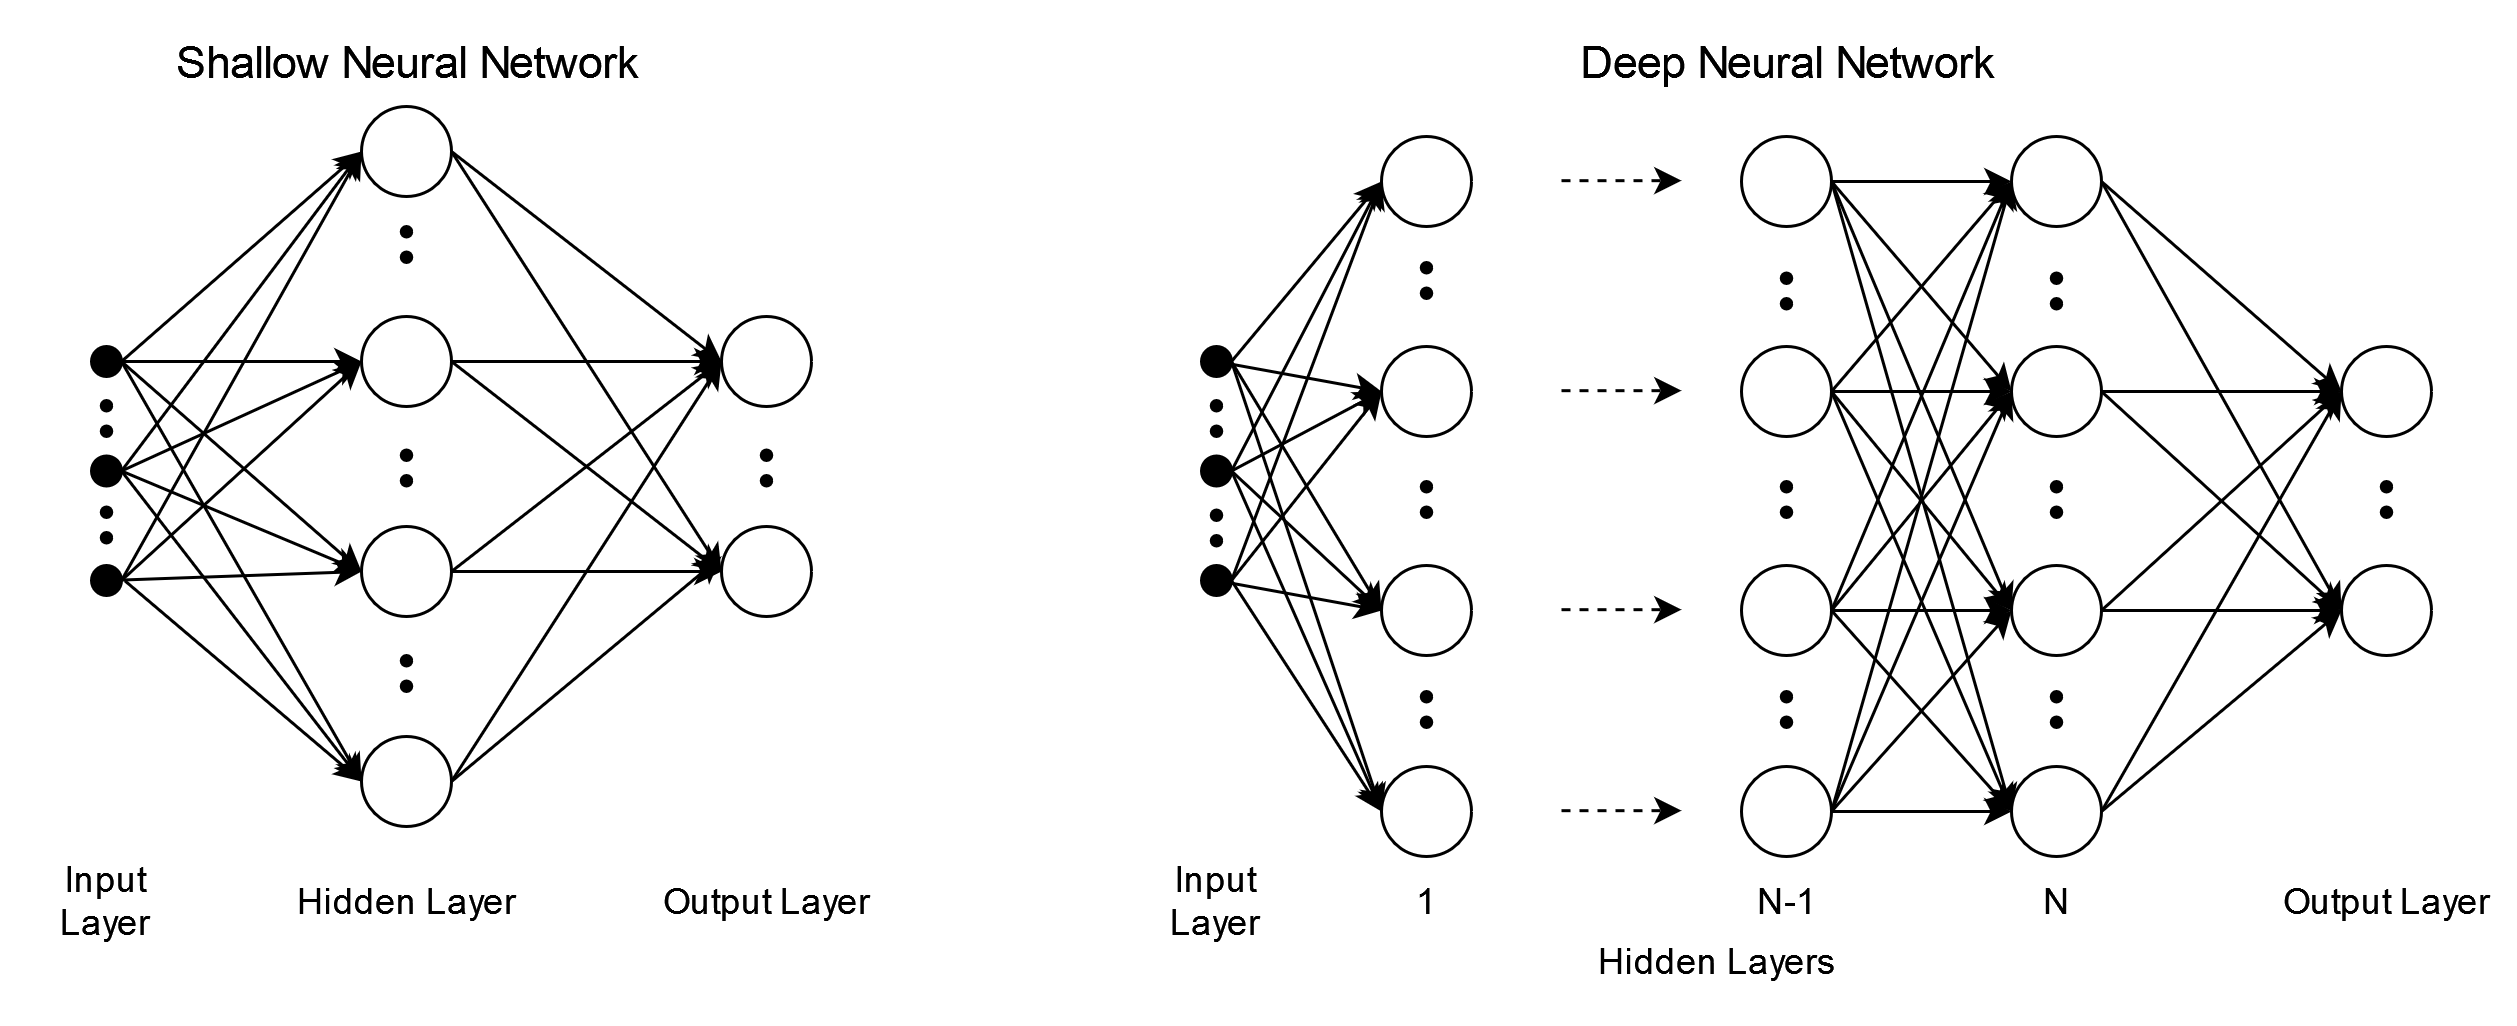
\includegraphics[width=\linewidth]{figures/2_theory/neuralNetDiagram.png}
    \caption[Ejemplos de la estructura de una ANN]{Ejemplos típicos de la estructura de una ANN, en este caso se tiene una red superficial o \textit{shallow} y una profunda o \textit{deep} \cite{annPictureSource}.}
    \label{fig:annExample}
\end{figure}

Cada neurona, como se ha descrito, recibe múltiples valores de entrada y produce un valor de salida que sirve como entrada para la siguiente capa. Además, cada neurona incorpora una función de activación no lineal\footnote{Si la función fuera lineal, toda la red se reduciría a una simple neurona, resultando en un modelo lineal, ya que la combinación de funciones lineales produce otra función lineal.}, la cual transforma las entradas en el valor de salida que se transmite. Esta función actúa de manera similar a un umbral, permitiendo que la red amplifique ciertas señales y suprima otras, en función de lo que se desea aprender. Dicho comportamiento se logra mediante la asignación de pesos a cada entrada de la neurona, junto con un valor adicional conocido como sesgo o bias. La modificación de los pesos y el sesgo permite ajustar la magnitud de la señal procesada por la función de activación. Un ejemplo visual de una neurona artificial se puede observar en la Figura \ref{fig:artificialNeuronExample}.

Existen numerosas funciones de activación, aunque las más comunes y ampliamente utilizadas incluyen la función sigmoidal o logística, la tangente hiperbólica y la ReLU (\textit{Rectified Linear Unit}). La elección de una función específica dependerá de la naturaleza y los requerimientos del problema a resolver.

\begin{figure}[h]
    \centering
    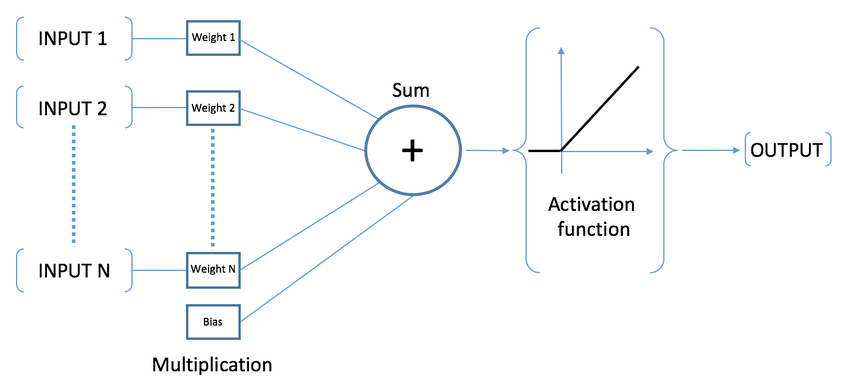
\includegraphics[width=\linewidth]{figures/2_theory/artificialNeuron.png}
    \caption[Ejemplo de una neurona artificial]{Ejemplo de una neurona artificial, los datos de entrada son multiplicados por los pesos y su resultado, junto con el sesgo (o \textit{bias}), son combinados linealmente. A continuación, son transformados por la función no lineal para proporcionar el valor salida de la neurona \cite{artificialNeuron}.}
    \label{fig:artificialNeuronExample}
\end{figure}

El aprendizaje en una ANN consiste esencialmente en ajustar los pesos y el sesgo de cada neurona para que, tras ser procesados por la función de activación, se puedan extraer y transformar las características más relevantes de los datos. El proceso inicia con la propagación hacia adelante (\textit{forward propagation}), en la cual los datos atraviesan la red desde la capa de entrada, pasando por las capas ocultas, hasta llegar a la capa de salida. Durante esta fase, se calculan los valores de salida de cada neurona, lo que finalmente permite obtener un resultado global de la red.

En este punto entra en juego la función de pérdida o error, cuya finalidad es medir qué tan bien ha aprendido la red. Existen diversas funciones de pérdida, y la elección de una en particular depende del tipo de problema y del enfoque de aprendizaje utilizado. A partir del valor de error obtenido, se aplica el algoritmo de retropropagación (\textit{backpropagation}), el cual calcula las derivadas de los pesos y sesgos respecto a dicho error. Posteriormente, mediante el uso de un algoritmo de optimización (\textit{optimizer}), se recalculan los valores de los pesos con el objetivo de minimizar el error de manera iterativa.

Este procedimiento, conocido como entrenamiento, permite que la red ajuste sus parámetros de manera progresiva hasta alcanzar un modelo que represente de manera óptima los patrones de los datos. Sin embargo, este enfoque de aprendizaje presenta un desafío fundamental en ML: el sobreentrenamiento u \textit{overfitting}. Este fenómeno ocurre cuando el modelo se ajusta excesivamente a los datos de entrenamiento, perdiendo capacidad de generalización. En tales casos, la red logra un error muy bajo en el conjunto de entrenamiento, pero su desempeño se deteriora considerablemente cuando se enfrenta a datos nuevos o no vistos previamente.

\subsection{Redes Neuronales Convolucionales}
\label{cnnDescription}
Las redes neuronales convolucionales (\textit{Convolutional Neural Network}, CNN) \cite{lecun_backpropagation_1989, leCUM_CNN} son un tipo de red neuronal artificial ampliamente utilizada en tareas de procesamiento, clasificación y segmentación de imágenes. Además, su aplicación se ha extendido a otras áreas como el procesamiento de texto, sonidos y, más recientemente, el análisis de superficies tridimensionales. A diferencia de una ANN tradicional, en la que todas las neuronas están completamente conectadas entre sí, una CNN introduce dos tipos adicionales de capas: capas convolucionales y capas de \textit{pooling}.

La estructura básica de una CNN puede visualizarse en la Figura \ref{fig:cnnExample}, donde se observa que la red está dividida en dos partes fundamentales. La primera parte está compuesta exclusivamente por capas convolucionales y de \textit{pooling}, cuyo propósito es extraer características relevantes de los datos de entrada. En la segunda parte, la estructura se asemeja a una ANN clásica, en la que las características extraídas se combinan de manera no lineal, permitiendo que la red realice tareas como la clasificación o detección de patrones dentro de los datos procesados.

\begin{figure}[h]
    \centering
    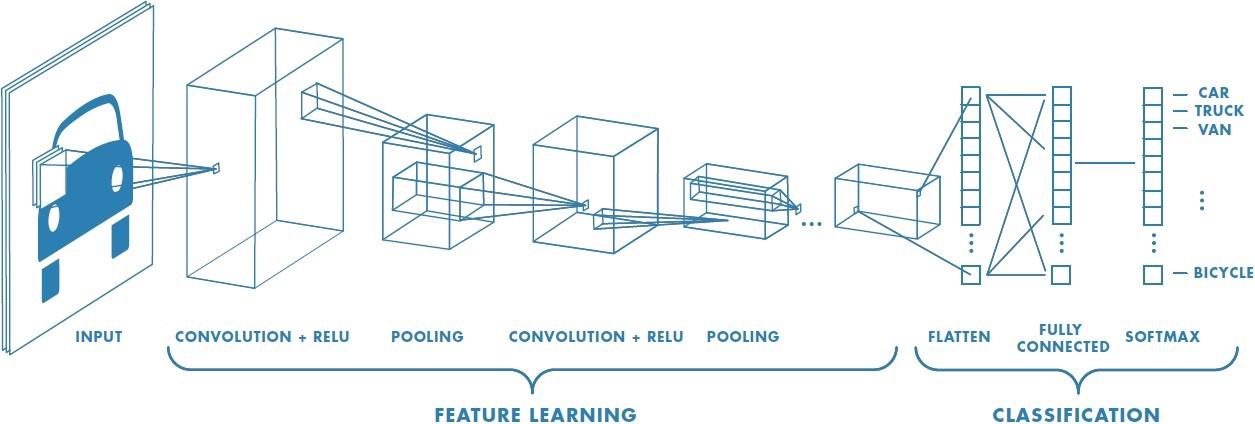
\includegraphics[width=\linewidth]{figures/2_theory/cnnExample.jpeg}
    \caption[Estructura básica de una red neuronal convolucional]{Estructura básica de una CNN donde se pueden apreciar las diferentes capas que la componen \cite{prabhu_understanding_2019}.}
    \label{fig:cnnExample}
\end{figure}

\subsection{Capa convolucional}
La capa convolucional es el elemento central de una CNN. A diferencia de una ANN clásica, en la que cada neurona está conectada con todas las neuronas de las capas vecinas, en una capa convolucional cada neurona está conectada únicamente a un vecindario local de neuronas. Esto es posible gracias a la operación de convolución, la cual permite procesar la imagen de entrada de manera eficiente\footnote{De aquí en adelante, se explicará el funcionamiento de la CNN clásica aplicada a imágenes, aunque su principio es similar en otros tipos de datos.}.

Una convolución consiste en un producto punto entre dos matrices (ver Figura \ref{fig:convolution} para una representación visual):
\begin{itemize}
    \item El \textit{kernel} (filtro o núcleo de la convolución), que es un conjunto de pesos que la red puede aprender y modificar.
    \item El campo receptivo (\textit{receptive field}), que es un fragmento de la imagen con el que el \textit{kernel} se multiplica en un momento dado.
\end{itemize}

El \textit{kernel} se desplaza por la imagen, comenzando en una esquina y moviéndose a través de filas y columnas de píxeles hasta recorrer toda la imagen. La matriz resultante de esta operación se procesa mediante una función no lineal, al igual que en una neurona clásica, y genera un mapa de características o mapa de activación, que servirá como entrada para la siguiente capa de la red.

Gracias a este proceso, la CNN puede capturar patrones espaciales y temporales en los datos mediante la aplicación de filtros relevantes. En las primeras capas convolucionales, la red aprende características de bajo nivel (como bordes y texturas), que luego se combinan en las capas siguientes para identificar características de alto nivel (como formas y estructuras más complejas).

Sin embargo, la aplicación directa de la convolución sobre una imagen reduce el tamaño del mapa de activación debido a la propia naturaleza del operador. Para mitigar esto, se pueden emplear técnicas como:
\begin{itemize}
    \item Relleno (\textit{padding}): Se añaden píxeles alrededor de la imagen utilizando información ya presente en ella, lo que permite mantener la misma dimensionalidad en la salida.
    \item Saltos (\textit{strides}): Se modifica el número de píxeles que avanza el kernel en cada paso, lo que puede reducir aún más la salida de la capa convolucional.
\end{itemize}

\begin{figure}[h]
    \centering
    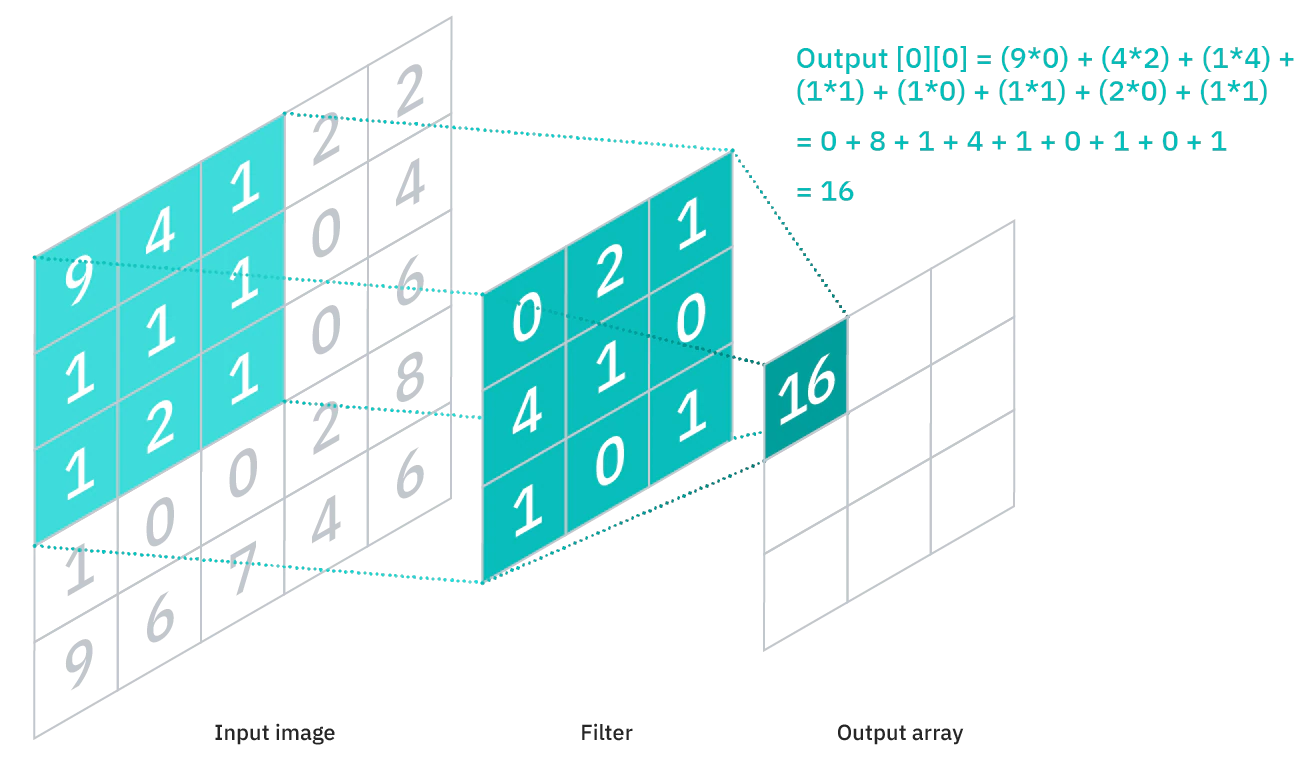
\includegraphics[width=\linewidth]{figures/2_theory/convolution.png}
    \caption[Ejemplo del operador de convolución]{Ejemplo de una convolución 2D con un \textit{kernel} $3 \times 3$. El campo receptivo para la neurona actual es la submatriz $3\times3$ de la imagen original con la que se está multiplicando el \textit{kernel} \cite{noauthor_what_2021}.}
    \label{fig:convolution}
\end{figure}

\subsection{Capa de \textit{pooling}}

Las capas de \textit{pooling} tienen como único objetivo reducir la dimensionalidad del mapa de activación generado por las capas convolucionales. Por ello, se insertan inmediatamente después de estas. Aunque las propias convoluciones pueden disminuir la resolución de los mapas de activación, el \textit{pooling} ofrece una forma más controlada de lograrlo y, además, mejora la extracción de características.

El \textit{pooling}, al igual que la convolución, utiliza un filtro o ventana que se desplaza a lo largo de los datos con un determinado salto (\textit{stride}). Sin embargo, en lugar de aplicar una operación de convolución, se realizan operaciones de reducción, como:
\begin{itemize}
    \item \textit{Max Pooling}: Se selecciona el valor máximo dentro de la ventana, lo que ayuda a preservar las características más relevantes y genera mayor invarianza a la traslación.
    \item \textit{Average Pooling}: Se calcula el promedio de los valores dentro de la ventana, lo que suaviza la salida y reduce el ruido en los datos.
\end{itemize}
La Figura \ref{fig:poolingExample} ilustra cómo funcionan estas operaciones.

\begin{figure}[h]
    \centering
    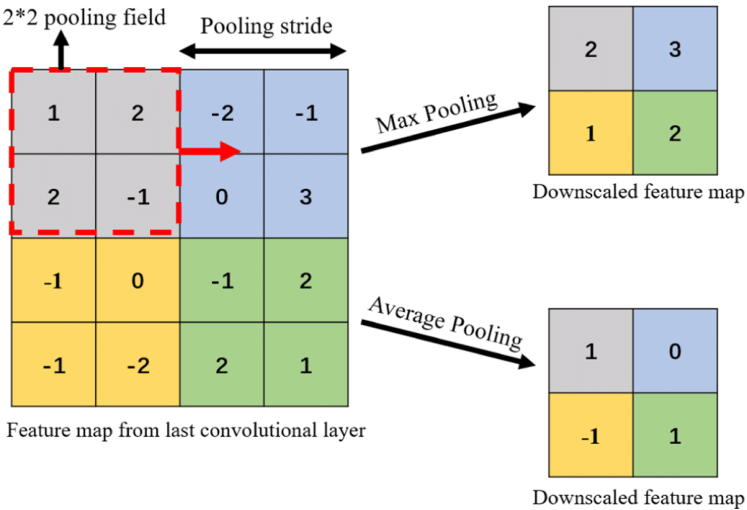
\includegraphics[width=\linewidth]{figures/2_theory/poolingExample.png}
    \caption[Ejemplo del operador de pooling]{Ejemplo de las operaciones de \textit{pooling} con un filtro $2\times2$ y \textit{stride} 2 \cite{pooling}.}
    \label{fig:poolingExample}
\end{figure}

Las capas convolucionales y de \textit{pooling} en conjunto conforman la sección de extracción de características en una CNN. Dependiendo de la complejidad del problema, el número de estas capas puede variarse para asegurar que la red extraiga las características esenciales necesarias para el aprendizaje.

\subsection{Capa totalmente conectada}
Las capas totalmente conectadas (\textit{fully connected} o \textit{dense layers}) aparecen después de las capas de convolución y \textit{pooling}, y constituyen la parte final de una CNN. Estas capas siguen la estructura de una ANN clásica, donde cada neurona está conectada con todas las neuronas de las capas adyacentes. Tomando como entrada las características extraídas y de ellas aprenden combinaciones no lineales. Gracias a esto, la red neuronal puede cumplir su objetivo, ya sea la clasificación o la regresión.

La última capa densa es la salida de toda la red. En esta etapa, se evalúa la función de pérdida, que mide la diferencia entre la predicción del modelo y la realidad. Luego, mediante \textit{backpropagation} y un algoritmo de optimización, los pesos de todas las neuronas de la red se ajustan durante el entrenamiento para minimizar el error.

\subsection{Regularización}
\label{subsection:regularization}
Como se ha comentado anteriormente, tanto las ANNs como las CNNs son propensas al fenómeno de sobreentrenamiento u \textit{overfitting}. La regularización es un método utilizado para combatir este fenómeno y en esencia lo que se quiere es controlar la complejidad del modelo, ya sea alterando los datos, el número de parámetros o el funcionamiento de la red. En general, la regularización es cualquier modificación que se puede realizar al modelo para que generalice mejor.

Se compone de múltiples técnicas diferentes, pero las más relevantes y utilizadas en CNNs son: La normalización, \textit{data augmentation}, la inicialización de los pesos y \textit{dropout}.

\subsubsection{Normalización}

\begin{figure}[h]
    \centering
    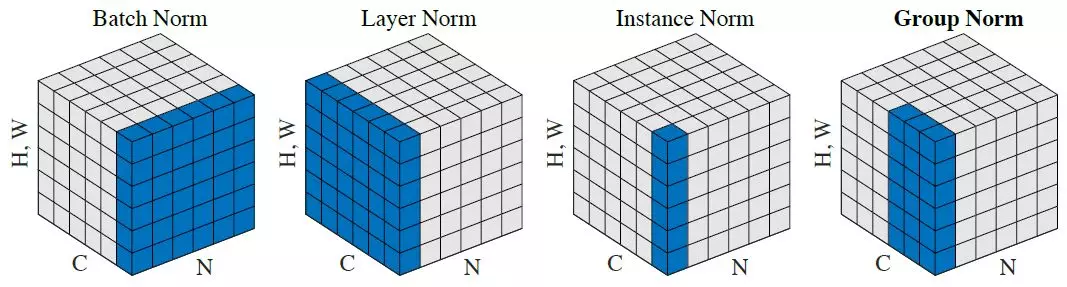
\includegraphics[width=\linewidth]{figures/2_theory/normTypes.png}
    \caption[Tipos de normalización]{Diferentes tipos de normalización. \textbf{H,W} indican la altura y anchura de la imagen, \textbf{C} indica los canales y \textbf{N} el número de lotes \cite{wu2018group}.}
    \label{fig:normTypes}
\end{figure}

La normalización es una técnica que estandariza los datos de manera que el valor medio de los mismos sea cercano a 0, con una desviación estándar cercana a 1, empíricamente se ha demostrado que esto mejora el rendimiento de las redes, pues evita que los pesos posean valores muy grandes, lo que afecta el cálculo de gradientes. 

Por lo general la normalización se aplica a las capas convolucionales de la red y la manera típica de utilizarla es haciendo uso de la normalización por lotes o \textit{batch normalization}, en donde se aplica la estandarización a una característica $i$-ésima de entrada calculando la media y desviación típica de todas las características $i$-ésimas del lote. Existe también la normalización por capa o \textit{layer normalization} que aplica la media y desviación típica por cada capa independiente del lote, la normalización por grupo o \textit{group normalization} que aplica la normalización a un grupo de canales pero no toda la capa entera. Por último se tiene la normalización por instancia o \textit{instance normalization} que normaliza cada canal por separado. El uso de un tipo u otro de normalización depende de la tarea a cumplir, pues se sabe que empíricamente diferentes tipos producen mejores modelos en diferentes problemas. Un ejemplo visual de todos los tipos de normalización se puede observar en la Figura \ref{fig:normTypes}. 

\subsubsection{\textit{Data Augmentation}}
El aumento de datos o \textit{data augmentation}, es una técnica para aumentar la cantidad de datos que se poseen de manera artificial, significa que, se generan nuevos datos de los ya presentes mediante la aplicación de transformaciones aleatorias pero realistas. Por ejemplo, escalados no uniformes de la imagen, rotaciones, traslaciones, adición de ruido o transformaciones de perspectiva. De esta manera se poseen más muestras de entrenamiento diferentes, lo que reduce la posibilidad de \textit{overfitting} porque la red tendrá más datos con los que trabajar y las modificaciones realizadas ayudan a la red a tener una idea más general de lo que se está aprendiendo.

\subsubsection{Inicialización de los pesos}
Como ha sido mencionado, las ANNs y CNNs utilizan pesos y sesgos en cada neurona, que son modificados en el entrenamiento por un algoritmo de optimización. Estos algoritmos necesitan un valor inicial que sea diferente de 0 al comienzo de dicho entrenamiento para funcionar, y la elección de estos valores afecta de gran forma al entrenamiento de la red, por lo tanto, se considera también como una técnica de regularización.

Se pueden inicializar los valores de forma aleatoria utilizando una distribución normal o uniforme que no toma en cuenta ningún parámetro de la red. Aún así, existen diversas heurísticas que se han desarrollado sobre los años que se ha comprobado mejoran el entrenamiento de los modelos. Por ejemplo, se tiene la inicialización Xavier \cite{glorot2010understanding} que parte de una distribución uniforme pero que toma en cuenta la cantidad de entradas que posee cada neurona, por lo que la inicialización está parcialmente guiada por la densidad de las capas. Otra inicialización heurística se denomina Kaiming \cite{he2015delving} y genera los valores por medio de una distribución normal acotada por el número de entradas de la capa.

\subsubsection{\textit{Dropout}}
La técnica de abandono o \textit{dropout} consiste en apagar o desactivar temporalmente cierta cantidad de neuronas en las capas totalmente conectadas de forma aleatoria durante el proceso de entrenamiento. La aplicación del \textit{dropout} hace que la red generalice mejor, pues las neuronas en una capa totalmente conectada tienden a generar una codependencia entre ellas, es decir, que ciertas neuronas se adaptan para contrarrestar los errores de otras neuronas y debido a que estos errores dependen de los datos de entrenamiento, no se generalizará bien para nuevos datos. Por lo tanto el \textit{dropout} permite evitar estas codependencias e impulsar el poder individual de cada neurona, lo cual aumenta el poder de generalización de la red.

\section{Clasificación Multietiqueta}
Como se ha descrito anteriormente, la clasificación emplea una variable de salida asociada a una variable discreta. Sin embargo, existe una extensión de esta idea en la que, para cada variable de entrada, pueden existir múltiples categorías asociadas que no se solapan entre sí. Este enfoque se conoce como clasificación multietiqueta (o multi-label classification).

En un problema de clasificación tradicional, cada instancia pertenece exclusivamente a una única clase dentro de un conjunto de categorías predefinidas. Por ejemplo, en la clasificación de imágenes de animales, un modelo puede etiquetar una imagen como \say{perro} o \say{gato}, pero no ambas a la vez. En contraste, en la clasificación multietiqueta, cada instancia puede estar asociada con múltiples categorías simultáneamente.

Un ejemplo común de este tipo de clasificación se encuentra en el etiquetado de imágenes en redes sociales, donde una misma foto puede contener etiquetas como \say{persona}, \say{playa} y \say{atardecer}. De manera similar, en el procesamiento de textos, un documento puede clasificarse dentro de varias categorías temáticas, como \say{tecnología}, \say{negocios} y \say{ciencia}, si su contenido abarca múltiples áreas.

Entre los algoritmos de ML más utilizados para la clasificación multietiqueta destacan los árboles de decisión, los métodos de vecinos más próximos, las máquinas de vectores de soporte (SVM) y las redes neuronales. En particular, las redes neuronales han logrado mejoras en el aprendizaje cuando se utiliza este método \cite{ranjan_hyperface_2019}.

Dado que el problema en cuestión involucra la clasificación de huesos de la sínfisis del pubis según las nueve categorías del método de Todd, es posible abordarlo mediante un enfoque de clasificación multietiqueta, donde bien se utilicen todas o algunas de las características en un único modelo de DL en vez de un modelo por cada característica.

\section{Grad-CAM}
El mapeo de activación de clase ponderado por gradiente (\textit{Gradient-weighted Class Activation Mapping}, Grad-CAM) \cite{selvaraju_grad_cam_2017} es una técnica ampliamente utilizada para interpretar el funcionamiento de las CNNs en tareas de clasificación de imágenes. Su propósito es identificar qué regiones de una imagen influyen en la decisión del modelo, proporcionando así una representación visual del proceso de clasificación.

Grad-CAM genera mapas de calor que destacan la relevancia de cada píxel en relación con una clase específica, generalmente aplicándose en la última capa convolucional de la red. Para ello, combina de manera lineal las activaciones de dicha capa, ponderadas por el gradiente de la salida correspondiente. Este cálculo permite resaltar las áreas de la imagen que impactan positiva o negativamente en la predicción del modelo. Finalmente, se conservan únicamente las contribuciones positivas, es decir, aquellas que refuerzan la decisión del modelo en favor de la clase seleccionada.

Por ejemplo observar la Figura \ref{fig__grad_cam} donde se tiene una fotografía de un perro y un gato (\ref{fig__grad_cam__og}). Si se estudia la clase \say{gato} con Grad-CAM, se obtiene un mapa de calor que indica que partes de la imagen han contribuido a que el modelo detecte al gato (\ref{fig__grad_cam__cat}). De igual forma si se estudia la clase \say{perro}, se obtiene un mapa de calor distinto indicando que partes influenciaron la detección del perro (\ref{fig__grad_cam__dog}).

La principal ventaja de Grad-CAM radica en su capacidad para generar explicaciones visuales, lo que facilita la comprensión de los factores que influyeron en la decisión de la red respecto a una clase específica. Además, este método es altamente versátil, ya que puede aplicarse a una amplia variedad de redes neuronales convolucionales sin necesidad de modificar su estructura, y su cálculo es relativamente sencillo.

Sin embargo, una de sus principales limitaciones es la dificultad para evaluar la precisión de las explicaciones generadas. En algunos casos, la interpretación de los mapas de calor puede no ser intuitiva o carecer de sentido lógico, lo que impide obtener resultados claramente interpretables \cite{molnar2025}.

\begin{figure}[!h]  
    \centering
    \begin{subfigure}{0.28\textwidth}
        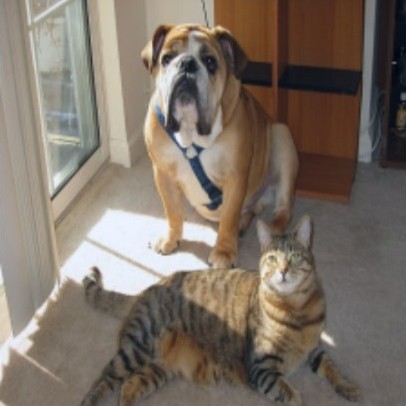
\includegraphics[width=\textwidth]{figures/2_theory/grad_cam__og.jpg}
        \begin{minipage}{.1cm}
            \vfill
            \end{minipage}
        \caption{Fotografía original.}
        \label{fig__grad_cam__og}
    \end{subfigure}
    \begin{subfigure}{0.28\textwidth}
        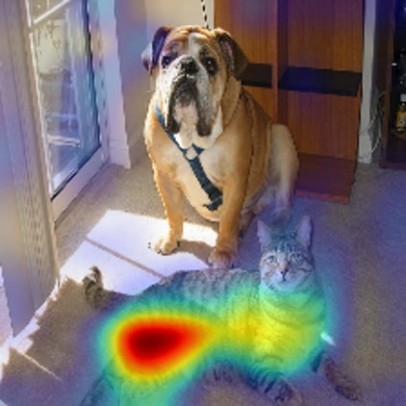
\includegraphics[width=\textwidth]{figures/2_theory/grad_cam__cat.jpg}
        \caption{Mapa de activación para la clase \say{gato}.}
        \label{fig__grad_cam__cat}
    \end{subfigure}  
    \begin{subfigure}{0.28\textwidth}
        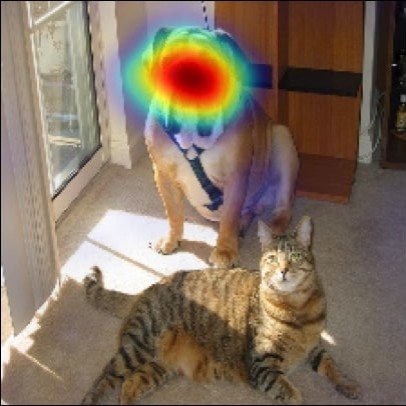
\includegraphics[width=\textwidth]{figures/2_theory/grad_cam__dog.jpg}
        \caption{Mapa de activación para la clase \say{perro}.}
        \label{fig__grad_cam__dog}
    \end{subfigure}    
    \caption{Ejemplo de funcionamiento de Grad-CAM \cite{selvaraju_grad_cam_2017}.}
    \label{fig__grad_cam}          
\end{figure}

\section{Búsqueda de Arquitectura Neuronal}
La búsqueda de arquitectura neuronal (\textit{Neural Architecture Search}, NAS) \cite{zoph_neural_2017} es un método que automatiza la generación de la estructura de una red neuronal. A diferencia de obtener una estructura por medio de conocimiento experto, se utilizan algoritmos para explorar e identificar la mejor arquitectura de red neuronal para una tarea específica. Este enfoque automatizado ayuda a optimizar el rendimiento, la velocidad y la eficacia \cite{ultralytics_busqueda_nas}.

El enfoque consiste en definir un espacio de búsqueda de posibles arquitecturas de red, establecer una estrategia para explorar este espacio y evaluar el rendimiento de cada arquitectura. Este proceso iterativo permite a NAS descubrir arquitecturas muy eficaces para tareas específicas que podrían no ser diseñadas intuitivamente por los humanos, y que a menudo igualan o superan las mismas tanto en exactitud como en uso de recursos y tamaño \cite{poyser_neural_2024}.

Si bien existen actualmente una gran cantidad de algoritmos NAS, estos se pueden clasificar en distintos grupos dependiendo de la estrategia utilizada para la exploración del espacio de búsqueda \cite{baymurzina_review_2022, white_neural_2023}.

\subsection{Métodos de búsqueda}
\subsubsection{Por métodos evolutivos}
Los métodos evolutivos o de \textit{neuroevolution} hacen uso de algoritmos evolutivos para la generación de la estructura de la red. La idea principal es la de ir modificando iterativamente la arquitectura por medio de una población de redes candidatas por el uso de operadores de cruce y mutación para incrementar su valor de evaluación o \textit{fitness}, en cada siguiente iteración se van cruzando las redes con el mejor \textit{fitness} para obtener descendientes hasta que se obtenga un valor deseado de \textit{fitness} o se llegue a un criterio de para definido. Notablemente, la función de optimización no tiene por qué ser diferenciable, por lo que resultan particularmente útiles para optimización multi objetivo. 

Este método ha demostrado obtener redes con la misma efectividad que las obtenidas por humanos, pero esto viene con el conocido alto coste computacional que requieren los algoritmos evolutivos. Adicionalmente existen los costos computacionales de entrenar desde cero cada integrante de la población por cada iteración para determinar su \textit{fitness}.

\subsubsection{Por optimización bayesiana}
La optimización bayesiana es un método para encontrar la mejor arquitectura de red utilizando un modelo probabilístico sustituto. Este modelo predice el rendimiento de distintas arquitecturas y se actualiza iterativamente a medida que se recopilan nuevos datos. Para decidir qué arquitecturas probar, se usa una función de adquisición, que equilibra la exploración (probar opciones nuevas) y la explotación (refinar las mejores opciones encontradas). Una vez seleccionada una arquitectura prometedora, se evalúa su rendimiento real y se incorpora esta información en el modelo. Este proceso se repite hasta alcanzar un criterio de parada definido.

Este método es muy popular en NAS debido a que, en comparación con otros métodos, obtiene arquitecturas buenas en pocas iteraciones y es capaz de soportar espacios de búsqueda complejos, aunque está limitada en escalabilidad y en la paralelización de la búsqueda.

\subsubsection{Por aprendizaje por refuerzo}
El método de aprendizaje por refuerzo (\textit{Reinforcement Learning}, RL) intenta mejorar la búsqueda en el espacio de soluciones utilizando un modelo controlador conocido como un \say{agente} que realiza una \say{acción} muestreando una arquitectura y recibe una \say{recompensa} que es alguna métrica de validación de la red neuronal, como por ejemplo el \textit{accuracy} de la misma. En este paradigma, el agente iterativamente aprende a generar la arquitectura que genere las mejores recompensas basándose en algoritmos de RL basados en políticas o en valores.

Este método se ha demostrado capaz de obtener redes con las mismas capacidades que las diseñadas a mano, con el mayor cuello de botella siendo la necesidad de reentrenar cada modelo para la siguiente iteración, aunque se han desarrollado variantes que permiten modificar una red parcialmente entrenada para ahorrar tiempo de cómputo.

\subsubsection{Por pesos compartidos}
Esta familia de métodos surge por los costos computacionales producidos por la necesidad de reentrenar cada red candidata desde cero. La solución propuesta permite que pesos de las neuronas estén compartidos entre diferentes redes.

Se puede realizar por el uso de una SuperRed (\textit{SuperNet}), donde un agente LSTM selecciona una subred para ser entrenada como una solución candidata al problema. De  esta forma las neuronas que son comunes para las distintas subredes van actualizándose en cada entrenamiento al mismo tiempo que el agente LSTM va aprendiendo qué subredes son las mejores para el problema. Si bien reduce substancialmente el tiempo de cómputo, poseen alto uso de memoria y necesitan ser cuidadosamente tuneadas, de lo contrario los pesos pueden interferirse entre sí provocando un colapso en su desempeño.

Otro método, denominado Búsqueda de Arquitectura Diferenciable (\textit{Differentiable Architecture Search}, DART), en vez de tratar el espacio de búsqueda como algo discreto, se relaja para volverlo continuo representando las operaciones candidatas (por ejemplo: convoluciones, pooling y saltos en las conexiones) como sumas ponderadas, permitiendo así hacer uso del \textit{backpropagation} para optimizar tanto los pesos de la red neuronal como la arquitectura misma. Reducen el tiempo de cómputo en comparación con otros métodos, pero de igual forma poseen un alto uso de memoria y son susceptibles a converger en operaciones demasiado simples.

\subsubsection{Por búsqueda aleatoria}
Este método es el más básico e ingenuo de los utilizados, se trata de seleccionar arquitecturas al azar de las posibilidades del espacio de búsqueda y quedarse con la que obtenga la mejor puntuación en la métrica seleccionada. Aunque se trate de un concepto bastante sencillo y que por lo general estos métodos se utilizan como bases para comparar los métodos anteriormente mencionados, se pueden obtener muy buenas arquitecturas si se ha diseñado el espacio de búsqueda correctamente.

\subsection{Espacios de búsqueda}
Hay que tomar en cuenta que las estrategias de búsqueda son independientes del espacio de búsqueda, la elección este espacio puede afectar drásticamente el desempeño de la red resultante, representa un importante compromiso entre el sesgo humano y la eficiencia de la búsqueda: si el tamaño del espacio de búsqueda es pequeño e incluye muchas decisiones seleccionadas manualmente, los algoritmos NAS tendrán más facilidad para encontrar una arquitectura de alto rendimiento. Por otro lado, si el espacio de búsqueda es grande y contiene bloques de construcción más primitivos, un algoritmo NAS necesitará ejecutarse durante más tiempo, pero existe la posibilidad de descubrir arquitecturas novedosas \cite{white_neural_2023}.

\subsubsection{Espacios de búsqueda basados en cadenas}
Los espacios de búsqueda basados en cadenas, como el nombre sugiere, tienen una topología sencilla: encadenar capas de operaciones para generar la arquitectura de la red. Son conceptualmente simples, lo cual los hacen fáciles de diseñar e implementar. También permiten que se encuentren con facilidad arquitecturas eficaces, pero por tener una topología tan sencilla es menos probable que se obtengan diseños de arquitecturas verdaderamente novedosas.

\subsubsection{Espacios de búsqueda basados en celdas}
Los espacios de búsqueda basados en celdas toma inspiración en el hecho que la mayoría de las arquitecturas del estado del arte para CNNs consisten en patrones repetidos múltiples veces, como por ejemplo, los bloques residuales en la familia de redes ResNets. Por lo tanto, en vez de intentar generar toda la red desde cero, se enfoca en buscar \say{celdas} relativamente pequeñas y apilarlas en secuencia para formar la arquitectura de la red. Cabe destacar que la forma de la red a gran escala se encuentra predefinida, pero cada bloque se puede componer de diferentes \say{celdas}. Son muy populares y pueden obtenerse con rapidez, pero como la macroestructura se encuentra ya fija, no permiten mucha expresividad y variación de las arquitecturas que se obtienen.

\subsubsection{Espacios de búsqueda jerárquicos}
A diferencia de los otros tipos de espacios de búsqueda, en lo que todo el diseño de la arquitectura es \say{plano} o diseñado en una sola capa, los espacios de búsqueda jerárquicos poseen múltiples niveles en los que se va definiendo la estructura de la red desde los parámetros más generales hasta los más específicos. Son extremadamente expresivos, permiten obtener redes complejas y diversas, además de que al tener la jerarquía se hace más efectivo la búsqueda del espacio lo que lo hace más eficiente también. Por otro lado, son bastante más complicados de diseñar e implementar.

\section{Representaciones 3D en \textit{Deep Learning}}
\label{3d_reps}
Las CNNs fueron originalmente diseñadas para procesar imágenes, es decir, datos bidimensionales organizados en estructuras regulares. Como consecuencia, aún no existe un consenso sobre la mejor manera de representar modelos tridimensionales en el contexto del \textit{Deep Learning}, dado que este tipo de datos suele presentar estructuras irregulares, lo que dificulta la adaptación de los métodos tradicionales. Además, la investigación en esta área es relativamente reciente.

No obstante, el desarrollo de dispositivos más accesibles para la digitalización y generación de modelos 3D a partir de objetos físicos, junto con el crecimiento en la cantidad de modelos tridimensionales generados por ordenador y la instauración del concurso anual \textit{3D Shape Retrieval Challenge} (SHREC) \cite{noauthor_shrec_nodate, noauthor_3dor2024_nodate}, han impulsado la exploración de diversas estrategias para representar información tridimensional de manera que pueda ser procesada mediante DL. Cada una de estas estrategias presenta ventajas y limitaciones particulares.

En la literatura, se han identificado cinco principales categorías de representaciones tridimensionales: datos en bruto, sólidos, superficies, estructuras de alto nivel y datos de múltiples vistas (véase Figura \ref{fig:3dTaxonomy}). Esta clasificación fue propuesta inicialmente por Ahmed et al. \cite{ahmed_survey_2019} y posteriormente ampliada por Gezawa et al. \cite{gezawa_review_2020} y Muzahid et al. \cite{muzahid_deep_2024}.

\begin{figure}[h]
    \centering
    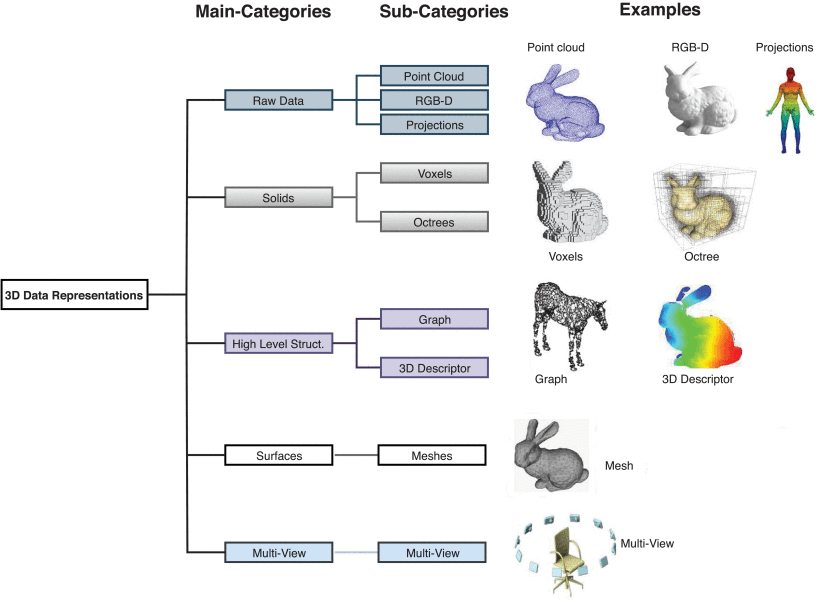
\includegraphics[width=\linewidth]{figures/2_theory/3Dtaxonomy.png}
    \caption[Taxonomía de las representaciones 3D para Deep Learning]{Taxonomía de las diferentes técnicas actuales en DL utilizadas para representar datos tridimensionales \cite{gezawa_review_2020}.}
    \label{fig:3dTaxonomy}
\end{figure}

\subsection{Datos en bruto}
Los datos en bruto corresponden a la información tridimensional obtenida directamente mediante métodos de escaneo, sin aplicar transformaciones significativas. Estos datos pueden ser capturados mediante dispositivos como el Microsoft Kinect o escáneres de luz estructurada, lo que permite representar la geometría de los objetos con un alto grado de fidelidad.

\subsubsection{Nube de Puntos}
La nube de puntos es una representación tridimensional compuesta por un conjunto de puntos sin estructura explícita, definidos por coordenadas espaciales, ya sea en un sistema cartesiano u otro sistema de referencia. Esta técnica tiene su origen en la fotogrametría y, más recientemente, en el escaneo mediante tecnología LiDAR.

Su principal ventaja radica en su facilidad de obtención y su fidelidad con los datos originales, ya que es una de las representaciones más cercanas a la captura en bruto. Sin embargo, su procesamiento es complejo debido a la ausencia de información sobre la conectividad entre los puntos, lo que puede generar ambigüedades en la forma real del objeto. Además, las nubes de puntos suelen contener datos incompletos o ruidosos, lo que dificulta la distinción entre información relevante y elementos espurios.

\subsubsection{Datos RGB-D}
Los datos RGB-D constituyen una representación tridimensional en la que se combina información cromática en formato RGB con un canal adicional de profundidad (D), que indica la distancia de cada píxel al sensor. Esta técnica fue popularizada por el Microsoft Kinect y proporciona una representación en 2.5D del objeto.

La principal ventaja de los datos RGB-D es la facilidad con la que pueden ser adquiridos y procesados, lo que ha permitido la creación de numerosos \textit{datasets} para su análisis. No obstante, su principal limitación radica en la falta de información geométrica completa, ya que no capturan la estructura tridimensional completa del objeto, restringiendo su aplicabilidad en tareas que requieren un modelado detallado de la forma.

\subsubsection{Proyecciones}
Las proyecciones permiten mapear información tridimensional en un plano bidimensional mediante la generación de vistas proyectadas del objeto. Estas proyecciones pueden ser de distintos tipos, siendo las cilíndricas y esféricas las más utilizadas debido a su invarianza frente a rotaciones alrededor del eje principal.

Entre sus ventajas destaca su capacidad para conservar las características más relevantes de la superficie 3D proyectada, además de facilitar el uso de modelos preentrenados en imágenes bidimensionales. Sin embargo, su aplicación en tareas complejas relacionadas con superficies tridimensionales es limitada, ya que la transformación a 2D conlleva la pérdida de información topológica fundamental.

\subsection{Sólidos}
Las representaciones de sólidos en modelos tridimensionales proporcionan detalles sobre el espacio que ocupa un objeto en tres dimensiones, es decir, indican si una región específica del espacio está ocupada o vacía por el objeto en cuestión. Estas representaciones se enfocan principalmente en describir tanto la estructura interna como la ocupación espacial del objeto.

\subsubsection{Vóxeles}
La representación mediante vóxeles puede pensarse como una cuadrícula regular en tres dimensiones, en la cual el modelo 3D está distribuido. Además, la información del punto de vista puede codificarse clasificando los vóxeles como visibles o no visibles desde dicho punto de vista.

Aunque los vóxeles ofrecen una representación completa del modelo, la necesidad de representar tanto las áreas ocupadas como las vacías del volumen conlleva un uso excesivo de memoria, lo que hace inviable su utilización en modelos de alta resolución debido a la gran demanda de recursos.

\subsubsection{Árbol octal}
El árbol octal es una representación más eficiente en comparación con la de vóxeles, ya que, en lugar de utilizar una cuadrícula regular, el tamaño de los vóxeles es variable. Los árboles octales modelan la información tridimensional mediante una estructura de datos jerárquica en forma de árbol, que describe la ocupación del objeto dentro de la escena 3D. Esta representación se basa en la descomposición recursiva de la escena en cubos, cada uno de los cuales tiene 8 subceldas (hijos) que pueden estar dentro o fuera del objeto.

Su principal ventaja radica en su mayor eficiencia en comparación con los vóxeles, permitiendo representar los detalles con mayor precisión y generar modelos de alta resolución. Sin embargo, su principal desventaja es la incapacidad para mantener con exactitud la geometría de ciertos objetos 3D, como es el caso de la suavidad en las superficies.

\subsection{Estructuras de alto nivel}
En tareas como la clasificación y la recuperación de formas tridimensionales, es necesario contar con representaciones que sean tanto concisas como detalladas de los modelos 3D. Estas representaciones permiten describir un objeto de manera que sea representativo de una categoría específica.

\subsubsection{Descriptor 3D}
Los descriptores 3D son representaciones simplificadas, generalmente creadas manualmente o \textit{handcrafted}, de los modelos 3D, que capturan las características geométricas o topológicas del objeto. Estos descriptores pueden derivarse de varias propiedades, como la geometría, la topología, la superficie, la textura o una combinación de todas ellas. Se pueden considerar como una "firma" que caracteriza de manera única un modelo 3D.

La principal ventaja es que facilitan el procesamiento y la computación de modelos 3D, siendo especialmente útiles en tareas de comparación, análisis y recuperación de formas tridimensionales, particularmente en contextos de aprendizaje no supervisado. Sin embargo, su mayor desventaja es que su utilidad disminuye en tareas de aprendizaje supervisado. Esto se debe a que el descriptor extrae características de los datos en bruto, lo que implica una abstracción adicional sobre los datos del modelo 3D. En un modelo supervisado, se estaría aprendiendo a partir de una abstracción de una abstracción, lo que puede resultar en la pérdida de información si la representación es demasiado simple o abstracta.

\subsubsection{Grafos}
La representación mediante grafos permite resumir la información tridimensional conectando las diversas formas a través de nodos y aristas. En este enfoque, los nodos del grafo corresponden a los vértices del modelo, mientras que las aristas representan las conexiones entre estos vértices. Los grafos pueden ser dirigidos o no dirigidos.

Dentro del contexto de redes neuronales sobre grafos, existen dos tipos principales de métodos: filtrado espectral y filtrado espacial. Los métodos de filtrado espectral se basan en la descomposición en valores y vectores propios de la laplaciana del grafo, utilizando este análisis para definir un operador similar a la convolución. En contraste, los métodos de filtrado espacial emplean filtros de paso alto y bajo como combinaciones lineales de las capas de la red. El proceso de aprendizaje se centra en el vecindario local de cada vértice, aplicando funciones no lineales a cada nodo del grafo.

Esta representación tiene la ventaja de que se puede aplicar a mallas 3D, y han mostrado resultados prometedores en diversas aplicaciones. Sin embargo, su principal desventaja radica en los altos costos computacionales y la dependencia del grafo base utilizado, lo que limita la capacidad de generalización entre diferentes dominios, haciendo que la transferencia de conocimientos entre ellos no siempre sea consistente.

\subsection{Superficies}
Este tipo de representación describe la superficie que cubre las partes internas de un objeto 3D mediante un conjunto de polígonos. Las superficies presentan la ventaja de ser simples, fáciles de procesar y de dibujar, ya que todas las superficies pueden representarse mediante ecuaciones lineales. Existen varios métodos de representación superficial, tales como las subdivisiones, las mallas paramétricas e implícitas. Sin embargo, la representación más popular y utilizada en el ámbito de DL es la malla poligonal, especialmente la malla triangular.

\subsubsection{Malla 3D}
Las mallas 3D están formadas por una combinación de vértices, aristas y caras. Cada vértice tiene asociada una lista de conectividad que indica cómo se conectan entre sí, y esta lista puede interpretarse como el conjunto de aristas que, a su vez, describen las caras de la malla.

La principal ventaja de las mallas 3D es su amplia adopción y relevancia en los gráficos por ordenador, tanto para almacenar descripciones de modelos 3D como para su visualización. No obstante, debido a su irregularidad y complejidad, el estudio de su aplicación en tareas de aprendizaje profundo no se había abordado satisfactoriamente hasta tiempos recientes. Hoy en día, se trata de una de las áreas más novedosas, con modelos que han alcanzado resultados satisfactorios, aunque con un alto consumo de recursos computacionales.

\subsection{Múltiples vistas}
Esta representación consiste en modelar un objeto 3D mediante un conjunto de imágenes tomadas desde diferentes puntos de vista, utilizando técnicas tradicionales de gráficos por ordenador. Posteriormente, estas imágenes se emplean como entradas para una CNN convencional.

La principal ventaja de esta representación es que permite aprovechar todas las técnicas y métodos ya existentes para CNNs basadas en imágenes, lo que facilita la utilización de modelos de alta resolución. Sin embargo, su mayor desventaja radica en la dificultad de determinar el número adecuado de puntos de vista a utilizar, así como en la pérdida de información que ocurre cuando partes del modelo 3D se solapan entre sí y quedan ocultas desde ciertos ángulos. Además, esta representación no conserva las propiedades geométricas intrínsecas del modelo 3D, y el uso de múltiples vistas conlleva un alto costo computacional. 

    % Estado del arte
    \chapter{Estado del Arte}

\section{Estimación de la edad}
La estimación de la edad, al ser un componente clave en la determinación del PB, ha captado un creciente interés por parte de la comunidad científica desde el siglo pasado, evidenciando una tendencia al alza en el número de publicaciones. En la Figura \ref{fig:scopusData} se muestra la evolución del volumen de publicaciones indexadas en la base de datos \textit{Scopus} que hacen referencia tanto a la AF como a la estimación de edad por medio de la cadena de búsqueda \ref{code__scopus_af}, registrándose un total de 1419 trabajos desde el siglo XX.

Sin embargo, y en línea con lo ya mencionado respecto a la limitada sofisticación tecnológica de esta disciplina, el número de publicaciones que integran técnicas de IA es considerablemente más reducido, al realizarse la consulta con la cadena \ref{code__scopus_af_ai} se identifican 71 artículos.

Finalmente, al acotar aún más la búsqueda a estudios que combinen IA con modelos tridimensionales para la estimación de edad mediante AF con la cadena \ref{code__scopus_af_ai_3d}, se obtienen únicamente ocho artículos. Esta escasa representación refuerza el carácter novedoso y pionero del presente trabajo.

\begin{lstlisting}[caption={Cadena de búsqueda de \textit{Scopus} para obtener publicaciones de AF que referencian la estimación de la edad.}, captionpos=b, label=code__scopus_af, style=Consola]
(TITLE-ABS-KEY (forensic AND anthropology AND age AND estimation))
\end{lstlisting}
            
\begin{lstlisting}[caption={Cadena de búsqueda de \textit{Scopus} para obtener publicaciones de AF que referencian la estimación de la edad y hacen uso de alguna técnica de IA}, captionpos=b, label=code__scopus_af_ai, style=Consola]
(TITLE-ABS-KEY (((deep AND learning) OR (machine AND learning) OR (soft AND computing) OR (artificial AND intelligence) OR (data AND mining)) AND forensic AND anthropology AND age AND estimation))
\end{lstlisting}
            
\begin{lstlisting}[caption={Cadena de búsqueda de \textit{Scopus} para obtener publicaciones de AF que referencian la estimación de la edad, hacen uso de alguna técnica de IA y utilizan datos 3D.}, captionpos=b, label=code__scopus_af_ai_3d, style=Consola]
(TITLE-ABS-KEY ( ((deep AND learning) OR (machine AND learning) OR (soft AND computing) OR (artificial AND intelligence) OR (data AND mining) ) AND forensic AND anthropology AND age AND estimation AND 3d))
\end{lstlisting}

\begin{figure}[h]
    \centering
    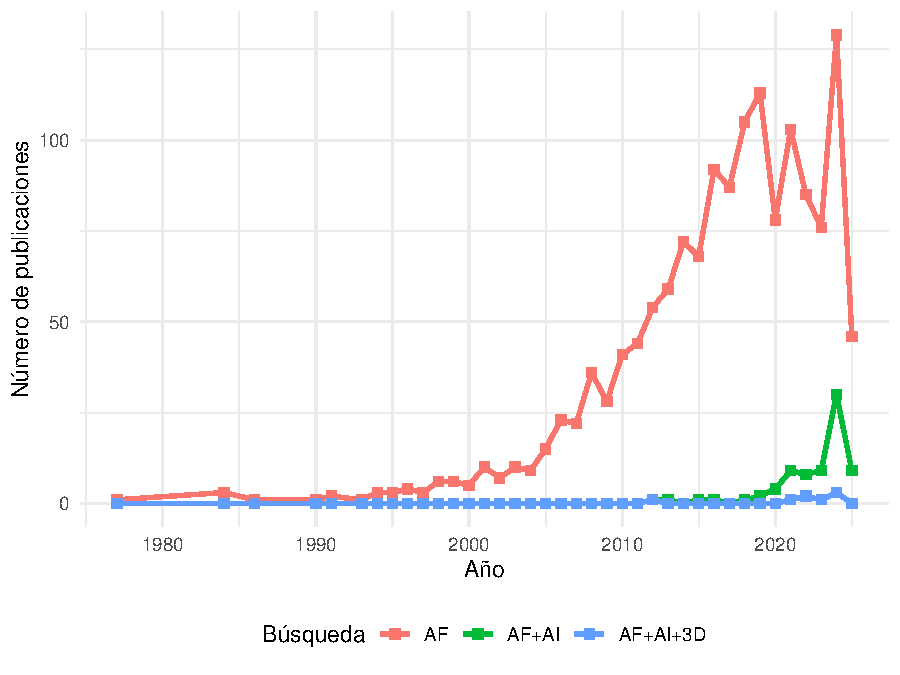
\includegraphics[width=\linewidth]{figures/3_sota/scopus_pubs.pdf}
    \caption[Publicaciones por año de AF, AF+IA y AF+IA+3D en Scopus]{Número de publicaciones en \textit{Scopus} en función del año a fecha de 08/04/2025. En {\color{Red} \textbf{rojo}} se muestran las publicaciones que mencionan AF y la estimación de la edad (1419 publicaciones), en {\color{LimeGreen} \textbf{verde}} aquellas que adicionalmente mencionan alguna técnica de IA (71 publicaciones) y en {\color{Blue} \textbf{azul}} aquellas que también mencionan el uso de 3D (8 publicaciones).}
    \label{fig:scopusData}
\end{figure}

A continuación se presenta el estado del arte de tanto en los métodos tradicionales utilizando la sínfisis del pubis y, brevemente, aquellos utilizados en otras estructuras óseas. Luego se presentan los métodos de estimación automáticos centrándose en la sínfisis del pubis con el uso de DL y modelos 3D.

\subsection{Métodos tradicionales para restos óseos}

En cuanto al cráneo, los métodos más comúnmente empleados para la estimación de la edad son los propuestos por Meindl y Lovejoy \cite{meindl1985ectocranial}, Acsádi y Nemeskéri \cite{acsadi1970history}, y Mann \cite{mann1991maxillary}. Estos enfoques se basan en el análisis del grado de osificación de las articulaciones fibrosas que conectan los distintos huesos del cráneo, conocidas como suturas craneales. De acuerdo con una revisión reciente \cite{ruengdit2020cranial}, estos métodos tienden a producir resultados erráticos y con baja precisión. Por ello, se recomienda su utilización únicamente como complemento de otros métodos basados en diferentes estructuras óseas. No obstante, el mismo estudio señala que la incorporación de nuevas tecnologías, como la tomografía axial computarizada, ha contribuido a reducir los márgenes de error en la estimación de edad, como se evidencia en trabajos como \cite{chiba2013age, boyd2015use}.

Respecto a las costillas, el método más utilizado es el desarrollado por İșcan y Loth \cite{icscan1984age, icscan1985age}, que se enfoca en los cambios morfológicos del extremo ventral de la cuarta costilla asociados al envejecimiento. Sin embargo, este método presenta diversas limitaciones, tales como sesgos poblacionales, escasa reproducibilidad entre distintas poblaciones y errores tanto intraevaluador como interevaluador de magnitud moderada \cite{fanton2010critical, hartnett2010analysis}. Actualmente, el método ha comenzado a incorporar de forma limitada técnicas de imagen como la tomografía axial computarizada para mejorar su precisión \cite{blaszkowska2019validation}.

En cuanto a la cara auricular del ilion, los métodos más utilizados para la estimación de la edad son los propuestos por Lovejoy \cite{lovejoy1985chronological} y por Buckberry y Chamberlain \cite{buckberry_age_2002}. Al igual que otros métodos tradicionales, estos también presentan limitaciones importantes en cuanto a la precisión de las estimaciones y están sujetos a diversos sesgos poblacionales \cite{falys2006auricular, michopoulou2017auricular}. En la actualidad, se ha intentado mejorar la fiabilidad de estos métodos mediante la incorporación de técnicas de imagen como la tomografía axial computarizada \cite{villa2013reliability, barrier2009age}, así como mediante la aplicación de enfoques analíticos basados en estadística bayesiana. No obstante, los resultados obtenidos con estos métodos complementarios han sido mixtos y no concluyentes \cite{nikita2018evaluation}.

\subsection{Métodos tradicionales utilizando la sínfisis del pubis}

La sínfisis del pubis constituye el hueso más comúnmente empleado en la estimación de la edad en contextos forenses, como se mencionó previamente en la Sección \ref{daIntro_ProblemDef}. En la actualidad, el método más difundido para este propósito es el propuesto por Suchey-Brooks \cite{RefWorks:RefID:20-brooks1990skeletal}, una variante modernizada del método original desarrollado por Todd. Ambos métodos se basan en la observación de características morfológicas específicas de la superficie de la sínfisis púbica (véase Tabla \ref{table:themBones}) para clasificar el hueso dentro de un determinado rango de edad. El método de Todd establece una clasificación en 10 fases o intervalos de edad, mientras que el método de Suchey-Brooks reduce esta categorización a 6 fases, aunque estas presentan un mayor grado de solapamiento entre sí. Los rangos definidos por ambos métodos pueden consultarse en las Tablas \ref{table:age_todd_} y \ref{table:age_suchey_brooks}.

\begin{table}[h]
\centering
\begin{tabular}{|c|c|}
    \hline
    \rowcolor[HTML]{D33333} 
    {\color[HTML]{FFFFFF} \textbf{Etapa}} & {\color[HTML]{FFFFFF} \textbf{Rango de Edad}} \\ \hline
    I & 18-19 \\ \hline
    II & 20-21 \\ \hline
    III & 22-24 \\ \hline
    IV & 25-26 \\ \hline
    V & 27-30 \\ \hline
    VI & 30-35 \\ \hline
    VII & 35-39 \\ \hline
    VIII & 39-44 \\ \hline
    IX & 45-50 \\ \hline
    X & 50+ \\ \hline
\end{tabular}
\caption{Rangos de edad del Método de Todd}
\label{table:age_todd_}
\end{table}

\begin{table}[h]
\centering
\begin{tabular}{|c|c|}
    \hline
    \rowcolor[HTML]{D33333} 
    {\color[HTML]{FFFFFF} \textbf{Etapa}} & {\color[HTML]{FFFFFF} \textbf{Rango de Edad}} \\ \hline
    I & 15-23 \\ \hline
    II & 19-34 \\ \hline
    III & 21-46 \\ \hline
    IV & 23-57 \\ \hline
    V & 27-66 \\ \hline
    VI & 34-86 \\ \hline
\end{tabular}
\caption{Rangos de edad del Método de Suchey-Brooks}
\label{table:age_suchey_brooks}
\end{table}

Según un metaanálisis reciente \cite{schanandore2022accuracy}, el método de Suchey-Brooks se posiciona como uno de los más precisos para la estimación de la edad en contextos forenses. No obstante, diversos autores recomiendan su aplicación con precaución debido a sus limitaciones inherentes \cite{priya2017methods}. En la actualidad, el uso de imágenes provenientes de tomografías computarizadas permite aplicar el método directamente sobre modelos volumétricos, replicando de manera virtual el análisis que tradicionalmente se realiza sobre el hueso físico. Algunos estudios \cite{wade2011preliminary,villa2013forensic,lottering2014morphometric,lopez2015image} han aprovechado esta tecnología para observar los cambios en la densidad ósea interna que ocurren con el envejecimiento, con el fin de refinar los procesos de estimación. Sin embargo, a pesar de la incorporación puntual de estas tecnologías, el método continúa dependiendo de características morfológicas subjetivas. Esta subjetividad conduce a que las estimaciones finales estén fuertemente influenciadas por la experiencia del perito, más que por una evaluación objetiva y sistemática de los datos, lo cual compromete tanto la efectividad como la credibilidad del proceso de estimación \cite{garvin_current_2012}.

\subsection{Métodos automáticos utilizando la sínfisis del pubis}

Los primeros intentos por reemplazar los métodos subjetivos en la estimación de edad a partir de la sínfisis del pubis surgen a inicios de la década de 2010 con el estudio realizado por Biwasaka et al. \cite{biwasaka2013three}. En dicho trabajo se calcula analíticamente la curvatura media de la superficie de la sínfisis del pubis, obtenida mediante escaneo 3D, para evaluar el grado de concavidad o convexidad del hueso en relación con los intervalos de edad definidos por el método de Suchey-Brooks. Aunque se utilizó una muestra de 145 huesos y se concluye que existe una relación entre las fases del método y la curvatura, el estudio no reporta métricas estadísticas cuantitativas que respalden los hallazgos.

Villa et al. \cite{villa2015quantitative} amplían el enfoque anterior al definir cinco variables derivadas del análisis de curvatura: la media del valor absoluto de la curvatura, el 10\% de curvaturas más altas, el 10\% más bajas, el porcentaje de superficie con curvaturas mayores que cero (regiones convexas) y el porcentaje con curvaturas entre $-0.01$ y $0.01$ (regiones planas). Se emplearon dos conjuntos de datos: uno con 24 huesos, que arrojó una correlación de Spearman moderada a fuerte ($\rho=0.60-0.93$), y otro con 98 huesos, con correlaciones más débiles ($\rho=0.29-0.51$), comparables a los valores alcanzados por métodos manuales, lo cual demuestra el potencial de este enfoque.

En Slice y Algee-Hewitt \cite{slice2015modeling} se introdujo una métrica denominada \textit{Slice Algee-Hewitt Score} (SAH-Score), basada en un análisis de componentes principales (PCA) aplicado a los vértices de mallas 3D de la sínfisis del pubis. Esta métrica cuantifica la complejidad superficial del hueso y se utiliza como predictor en un modelo de regresión lineal para estimar la edad. Con una muestra de 41 huesos, se obtuvo un error cuadrático medio (RMSE) de 17.15 años, con predicciones que coinciden razonablemente con los intervalos del método de Suchey-Brooks.

Stoyanova et al. \cite{stoyanova2015enhanced} emplean el algoritmo \textit{Thin Plate Splines} (TPS) para estimar la energía de flexión (\textit{bending energy}, BE) requerida para transformar una superficie plana en la forma tridimensional del hueso. Esta métrica se usa en un modelo de regresión lineal entrenado con 44 mallas, obteniendo un RMSE de 19 años. En un trabajo posterior \cite{stoyanova2017computational}, los autores combinan múltiples características (SAH-Score, BE y curvatura del borde ventral) para entrenar un modelo de regresión multivariable con 93 muestras, logrando un RMSE entre 13.7 y 16.5 años.

Villar et al. \cite{villar2017first} utilizan Árboles de Decisión Difusos (\textit{Fuzzy Decision Trees}, FDT) para generar reglas que permitan clasificar los huesos en los intervalos de edad del método de Todd, usando 74 muestras etiquetadas por dos expertos. El modelo alcanza un error absoluto medio (MAE) de 1.68 años respecto al intervalo correspondiente, aunque el número reducido de muestras impidió cubrir todos los rangos etarios.

En Gámez-Granados et al. \cite{granados} se propone un sistema explicable basado en reglas utilizando el clasificador ordinal NSLVOrd \cite{gamez2016ordinal}, el cual clasifica 892 muestras de sínfisis del pubis dentro de los 10 intervalos definidos por Todd, utilizando las nueve características tradicionales etiquetadas por expertos. Aunque el enfoque es de clasificación, puede adaptarse para predecir directamente la edad. El modelo reporta un RMSE de 12.34 años y un MAE de 10.38 años.

Kotěrová et al. \cite{kotverova2018age} exploran nueve métodos de regresión aplicados a características extraídas manualmente por expertos. Con una muestra de 941 huesos, la regresión lineal múltiple ofrece el mejor desempeño, con un RMSE de 12.1 años y un MAE de 9.7 años. En una extensión del estudio \cite{koterova_computational_2022}, se incorporan mallas 3D y se introducen dos nuevos enfoques: uno que caracteriza la superficie del hueso mediante la energía de Dirichlet, y otro basado en una CNN entrenada con múltiples proyecciones 2D del modelo 3D. Los mejores resultados obtenidos son un MAE de 11.7 y 10.6 años, respectivamente.

Por último, Bermejo et al. \cite{bermejo_interpretable_2025} proponen un método semi-automático e interpretable, basado en regresión simbólica obtenida mediante Programación Genética, utilizando como entrada las nueve características del método de Todd. El mejor modelo generado reporta un MSE de 10.81 años y un MAE de 8.55 años. Aunque estos resultados representan una mejora frente al método propuesto por Kotěrová, los autores consideran ambos enfoques como equivalentes y complementarios, dado que el modelo de Bermejo requiere el etiquetado experto de las características, mientras que el de Kotěrová es completamente automático.

Los tres últimos estudios mencionados son los más cercanos al enfoque de este TFM. En \cite{koterova_computational_2022} se emplea una CNN para extraer automáticamente características de la sínfisis del pubis a partir de un modelo 3D, aunque con el objetivo de estimar directamente la edad, a diferencia del presente proyecto, cuyo objetivo es clasificar el hueso según las características del método de Todd. En esta línea, los trabajos de \cite{villar2017first} y \cite{bermejo_interpretable_2025} sí hacen uso explícito de dichas características, pero partiendo de información etiquetada por expertos. Ambos enfoques permiten obtener reglas explicables para clasificar un hueso dentro de los intervalos de edad, o bien estimar un valor numérico de edad, pero no permiten identificar directamente las características morfológicas en la sínfisis del pubis. En este sentido, el presente trabajo se plantea como pionero, ya que, según la literatura consultada, no existe otro estudio que utilice técnicas de DL para extraer automáticamente las características de Todd a partir de modelos 3D.

\section{Representaciones 3D en \textit{Deep Learning}}
Como se discutió en la Sección \ref{section2:3dreps}, existen múltiples formas de representar datos tridimensionales para su utilización en técnicas de DL. En esta sección se analiza cuál de estas representaciones resulta más adecuada para la extracción automática de características morfológicas orientadas a la estimación de la edad, y se presentan los avances más recientes asociados a dicha representación.

La representación mediante nubes de puntos es la más sencilla, ya que consiste únicamente en un conjunto de coordenadas tridimensionales. Sin embargo, esta simplicidad implica que conceptos clave como la vecindad local y la conectividad entre puntos no están bien definidos. Esto dificulta la aplicación directa de operaciones típicas de CNNs, generando ambigüedades que afectan negativamente el rendimiento del modelo, especialmente en escenarios que requieren un alto nivel de detalle. Por estas razones, esta representación se descarta para este trabajo.

La representación RGB-D, aunque útil para algunas aplicaciones, es esencialmente una representación 2.5D y, por lo tanto, no tiene la capacidad de capturar completamente la complejidad de la geometría tridimensional. Dado que el objetivo es analizar en detalle la morfología ósea, esta representación también se descarta.

Las proyecciones y vistas múltiples permiten aprovechar arquitecturas clásicas de CNNs mediante la conversión del objeto 3D en una o varias imágenes 2D. Sin embargo, este enfoque conlleva pérdida de información topológica al realizar la proyección, y puede presentar problemas en superficies complejas donde partes del modelo ocluyen otras, generando aún más pérdida de información. Por ello, ambas representaciones se descartan igualmente.

Los descriptores 3D simplifican un modelo tridimensional en una representación compacta o \say{firma}, que resulta útil para tareas de reconocimiento global. Sin embargo, dado que este trabajo se enfoca en analizar detalladamente la topología de la superficie ósea, esta simplificación resulta inadecuada. Además, los descriptores son más eficaces en tareas de aprendizaje no supervisado que en supervisado, lo cual refuerza su exclusión. Por motivos similares, las representaciones basadas en grafos también se descartan, ya que requieren una transformación intermedia del modelo 3D que complica el tratamiento directo de su geometría.

Las representaciones volumétricas, como los vóxeles, permiten describir el volumen completo del objeto en una rejilla tridimensional. Sin embargo, esta aproximación tiene un elevado coste computacional debido a la necesidad de realizar operaciones sobre espacios vacíos, lo que incrementa significativamente el uso de memoria. Además, este tipo de representación no permite capturar con suficiente precisión los detalles finos de la superficie, lo que la hace inadecuada para el problema planteado.

La representación seleccionada en este trabajo es la de mallas poligonales tridimensionales. Estas son ampliamente utilizadas en el ámbito de la informática gráfica, lo que ha dado lugar a una gran variedad de herramientas y algoritmos para su procesamiento y análisis. Además, la mayoría de escáneres 3D empleados en AF generan directamente este tipo de representación, lo que facilita el flujo de trabajo. Las mallas son una representación eficiente y precisa: en zonas lisas y planas se utilizan pocos polígonos, mientras que en zonas con geometría compleja la densidad de polígonos aumenta, permitiendo capturar detalles intrincados. Desde el punto de vista del procesamiento mediante CNNs, las mallas ofrecen una ventaja adicional, ya que proporcionan información explícita sobre la conectividad entre vértices, lo que permite definir vecindarios locales de forma natural y estructurada.

\subsection{Mallas poligonales}
\label{section3:meshes}

En el trabajo pionero de Feng et al. \cite{feng2019meshnet} se propone MeshNet, el primer \textit{framework} basado en CNNs diseñado para procesar directamente mallas 3D. En este enfoque, la unidad básica de procesamiento no son los vértices ni los vóxeles, sino las caras triangulares de la malla, las cuales permiten mantener la conectividad topológica y facilitan la definición de operaciones análogas a las convoluciones en imágenes, donde los píxeles tienen vecindarios bien definidos.

Cada cara triangular es descrita por dos tipos de características, que funcionan como el análogo del valor RGB en imágenes: características espaciales y características estructurales.
\begin{itemize}
    \item Las características espaciales se calculan a partir de la posición del centroide de cada triángulo, representando su ubicación en el espacio.
    \item Las características estructurales se dividen en dos componentes: una que captura la estructura interna de la cara (por ejemplo, ángulos internos o proporciones entre lados), y otra que captura la estructura externa, que examina el vecindario local de cada cara, permitiendo aprender sobre la disposición relativa entre caras adyacentes.
\end{itemize}
Además, se redefine la operación de convolución para que trabaje de forma coherente con estas representaciones. El bloque convolucional propuesto consta de dos partes:

\begin{itemize}
    \item Una combinación de características espaciales y estructurales, que permite mezclar la posición con la forma local del triángulo.
    \item Una agregación estructural, que aprende a fusionar la información del vecindario de caras.
\end{itemize}
Ambas operaciones generan nuevas representaciones que se pasan al siguiente bloque de la red, permitiendo una jerarquía de aprendizaje similar a las CNNs tradicionales.

Para la validación del modelo, se utilizó el conjunto de datos ModelNet40 \cite{wu20153d}, una base de datos ampliamente utilizada en tareas de clasificación de objetos 3D. MeshNet alcanzó un 91.9\% de precisión en la tarea de clasificación, superando a modelos basados en nubes de puntos, representaciones volumétricas y métodos basados en múltiples vistas.

En Hanocka et al. \cite{hanocka2019meshcnn} se propone otro \textit{framework} denominado MeshCNN, publicado casi en paralelo con MeshNet, con solo unos meses de diferencia. A diferencia de MeshNet, que toma como unidad básica de procesamiento las caras triangulares, MeshCNN utiliza las aristas que conectan los vértices de la malla como unidad convolucional, lo que constituye el análogo al píxel en una imagen. En lugar de describir las caras con múltiples tipos de descriptores, cada arista es caracterizada mediante un vector de cinco componentes, compuesto por atributos geométricos específicos de la arista que son invariantes a traslación y rotación. Esto permite realizar operaciones de convolución de manera más directa y robusta frente a transformaciones espaciales. Una de las contribuciones más importantes de MeshCNN es la implementación de una operación de \textit{pooling} adaptativo, donde la red aprende automáticamente qué regiones de la malla puede simplificar y cuáles debe preservar, optimizando así la tarea de aprendizaje.

Los experimentos se realizaron en distintos conjuntos de datos, obteniendo un 98.6\% de \textit{accuracy} en SHREC30 \cite{lian2011shape} y un 92.16\% en un conjunto de cubos esculpidos con diferentes formas \cite{latecki2000shape}.

En Schneider et al. \cite{schneider_medmeshcnn_2021} se introduce MedMeshCNN como una extensión de MeshCNN enfocada en reducir el elevado consumo de memoria de la implementación original. Esta optimización se logra mediante modificaciones en la operación de \textit{pooling}, con énfasis en aplicaciones médicas, particularmente en tareas de segmentación de mallas 3D. Para su validación, se utilizaron 94 mallas de aneurismas intracraneales: 65 provenientes del conjunto de datos AneuRisk65 \cite{sangalli2014aneurisk65} y el resto provistas por el Hospital Universitario de Magdeburgo, Alemania. Se reporta un índice de Jaccard promedio de 63.24\% en todas las clases, con un 71.4\% específicamente para la segmentación de aneurismas, concluyéndose que el \textit{framework} tiene potencial para aplicaciones en el ámbito médico.

De forma pararela en \cite{mandado_surface_2021}, se presenta MeshCNN+, otra variante cuyo objetivo es también mitigar el alto uso de memoria de MeshCNN, mediante una nueva implementación del \textit{pooling} y la posibilidad de entrenamiento distribuido en múltiples máquinas. Este estudio también se centra en tareas de segmentación y utiliza el conjunto de datos ABC \cite{Koch_2019_CVPR}, que contiene más de un millón de mallas generadas mediante software de diseño asistido por computadora (CAD). El modelo alcanzó una \textit{accuracy} del 86.2\%, aunque se observó que tenía dificultades para segmentar clases poco representadas en la superficie de las mallas.

Por último, Kim y Chae \cite{kim_exmeshcnn_2022} introducen ExMeshCNN, una expansión y, al mismo tiempo, una mezcla entre las propuestas de MeshNet y MeshCNN, ya que combina la extracción de características tanto de las caras triangulares como de las aristas. Para ello, la capa inicial de cualquier modelo basado en esta técnica incorpora dos extractores de características geométricas y geodésicas a partir de las caras triangulares. Estos extractores, denominados descriptores, actúan como filtros de convolución 1D con parámetros entrenables. Las capas posteriores aplican convoluciones 1D sobre las caras triangulares y sus vecindades locales.

A diferencia de MeshCNN, que emplea operaciones de \textit{pooling} para aportar explicabilidad al modelo, ExMeshCNN permite aplicar técnicas como Grad-CAM gracias al uso de convoluciones 1D, lo que posibilita identificar directamente qué caras tienen mayor relevancia en la generación de una salida específica.

En los experimentos realizados con los conjuntos de datos ModelNet40 y Manifold40, ExMeshCNN alcanzó los mejores resultados reportados hasta la fecha, con 93\% y 93.4\% de \textit{accuracy} respectivamente, superando a modelos como MeshCNN y MeshNet++. De igual forma, en los conjuntos SHREC11 y el de cubos esculpidos, alcanzó un \textit{accuracy} del 100\%, posicionándose así como el \textit{framework} actual de referencia en el uso de \textit{Deep Learning} sobre mallas 3D.

    % Metodología 
    \chapter{Materiales y Métodos}

\section{Materiales}
\label{section4:materials}
Para la realización de este TFM se dispone de una colección de 986 mallas 3D de la sínfisis del pubis en formato OBJ. Se tratan de 493 huesos izquierdos y 493 derechos, con un rango de edades entre los 18 y 60 años, provenientes de países mediterráneos desarrollados, como España. Estas mallas fueron escaneadas por el personal del Laboratorio de Antropología Física del Departamento de Medicina Legal, Toxicología y Antropología Física de la Universidad de Granada. Además de la digitalización tridimensional, el equipo del laboratorio examinó cuidadosamente cada una de las muestras y etiquetó manualmente los atributos correspondientes a las características morfológicas observables en la superficie de la sínfisis del pubis así como la edad real de fallecimiento de los individuos, datos que también han sido provistos dentro de un fichero de Microsoft Excel. Se utilizaron las características y atributos propuestos por Villar et al. \cite{villar2017first} descritas en el atlas propuesto por Irurita et al. \cite{irurita2025pubic}, que se pueden visualizar en la Tabla \ref{table:themBones}.


\begin{figure}[htbp]
    \centering
    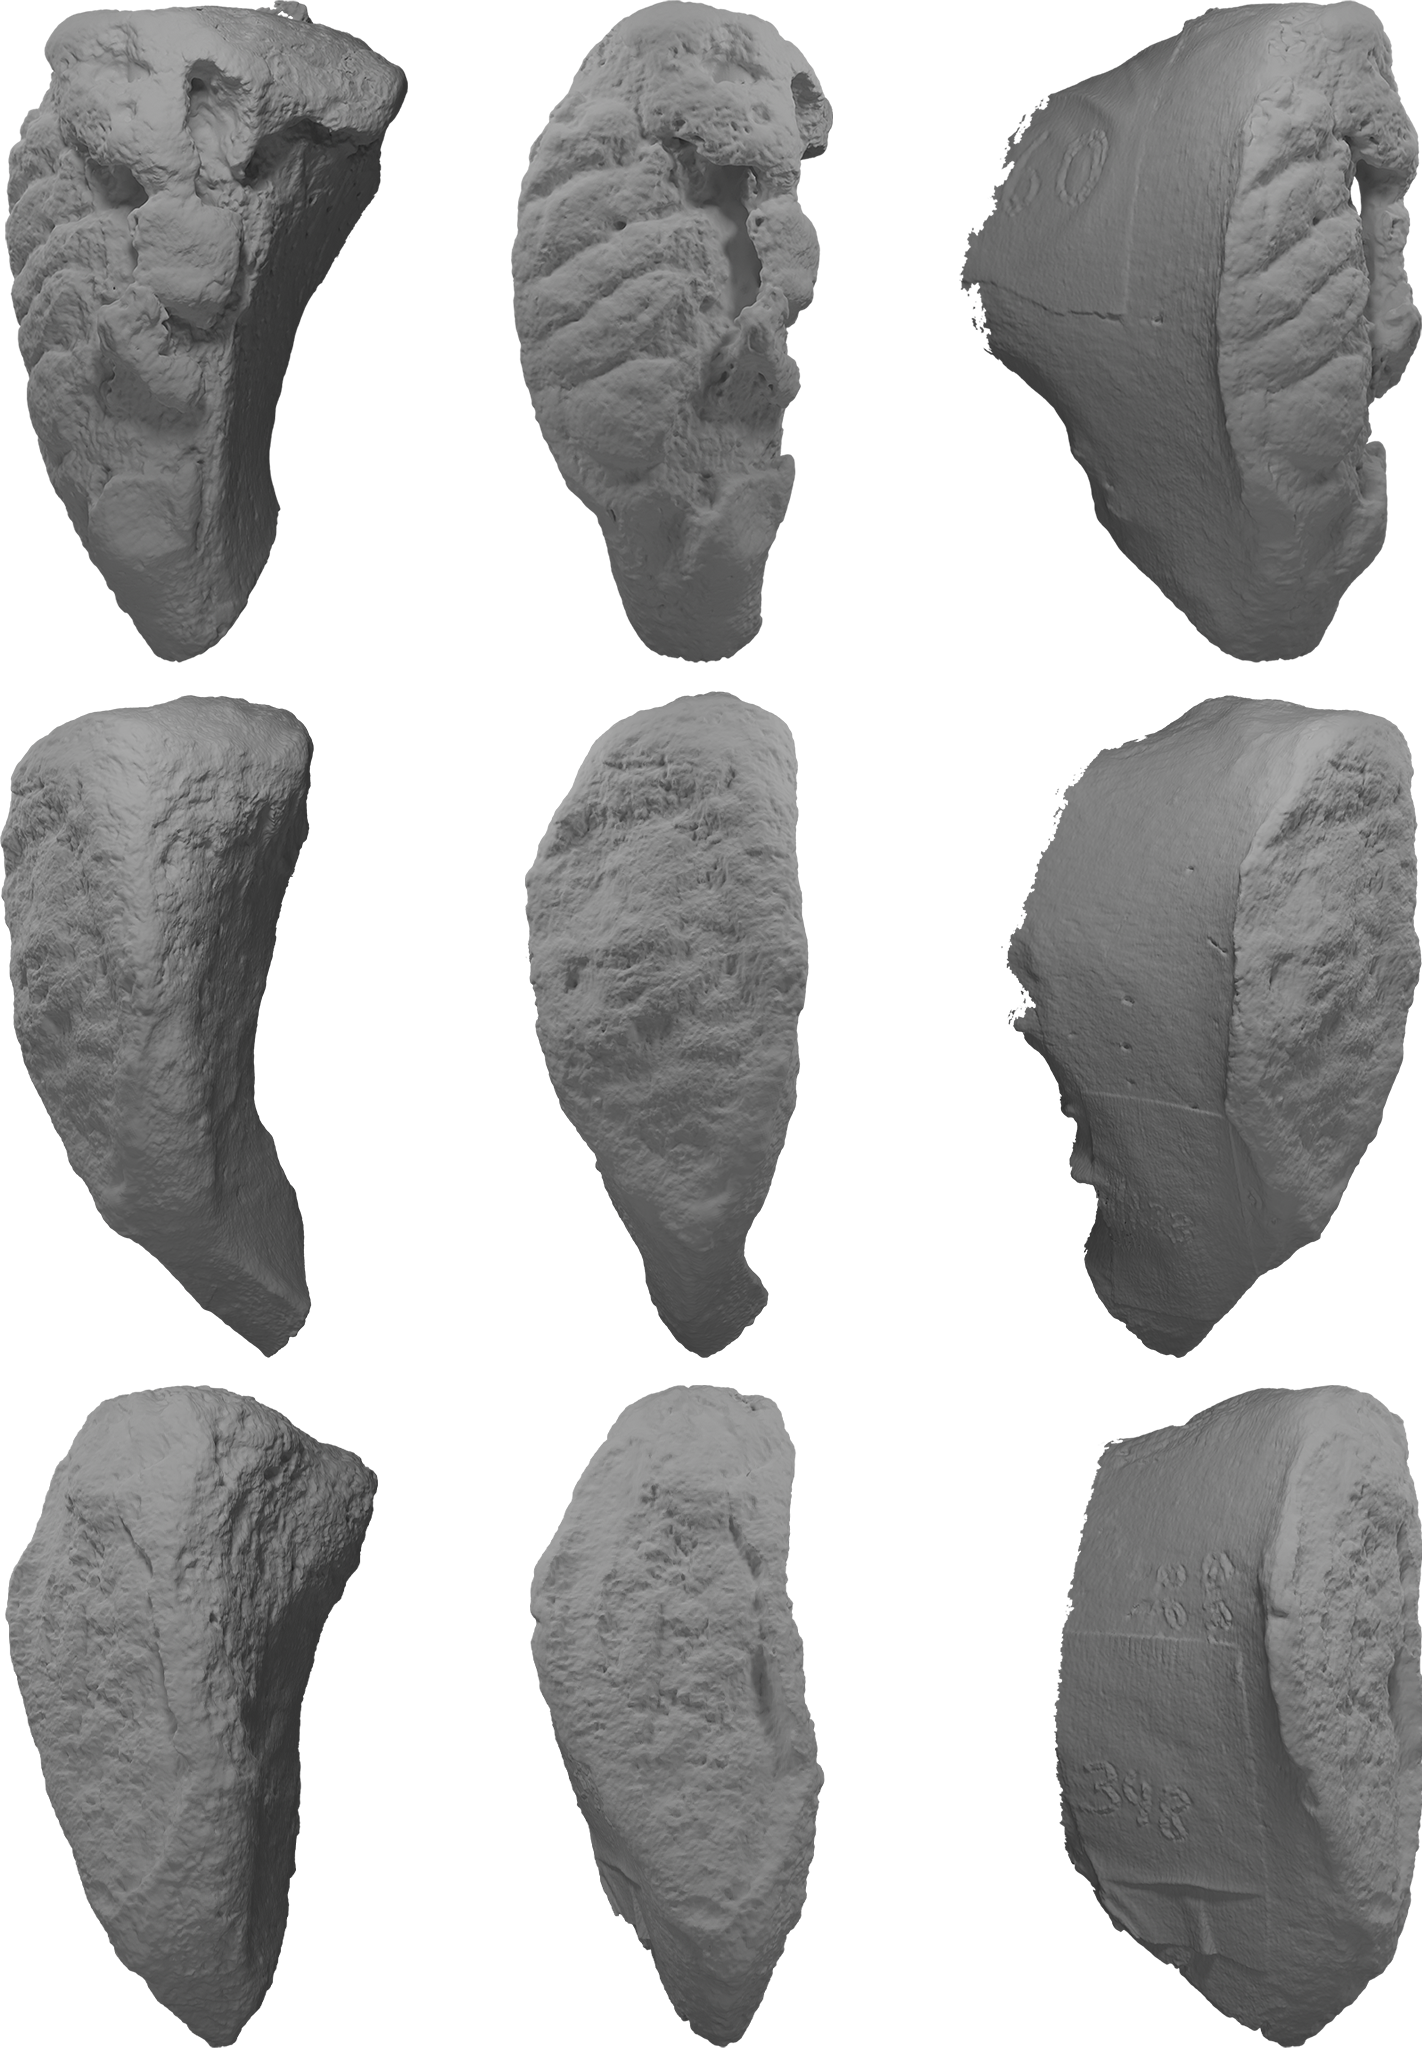
\includegraphics[width=0.75\linewidth]{figures/4_materials-methods/pb-examples.png}
    \caption[Ejemplos de mallas 3D de la sínfisis del pubis]{Ejemplos de mallas 3D de la sínfisis del pubis. Se presentan tres muestras distintas, renderizadas con iluminación fotorrealista desde tres ángulos relativos a la cara sinfisaria o articular del hueso: vista lateral izquierda (a), frontal (b) y lateral derecha (c). Obsérvese la complejidad de la superficie ósea, la cual ha sido capturada con alta fidelidad por el escáner 3D.}
    \label{pb_3dexamples}
\end{figure}

A partir de este punto, se utilizarán las abreviaciones en inglés de dichas características con el fin de facilitar legibilidad del texto. La correspondencia entre las abreviaciones y su nombre en castellano puede consultarse en la Tabla \ref{table4:chars_short_names}.

\begin{table}[h]
    \centering
    \begin{tabular}{|c|c|c|}
    \hline
    \rowcolor[HTML]{D33333} 
    {\color[HTML]{FFFFFF} Nombre Castellano} & {\color[HTML]{FFFFFF} Nombre Inglés} & {\color[HTML]{FFFFFF} Abreviación} \\ \hline
    Crestas y Surcos & \textit{Articular Face} & \textbf{AF} \\ \hline
    Porosidad Irregular & \textit{Irregular Porosity} & \textbf{IP} \\ \hline
    Borde Superior & \textit{Upper Symphysial Extremity} & \textbf{USE} \\ \hline
    Nódulo Óseo & \textit{Bony Nodule} & \textbf{BN} \\ \hline
    Borde Inferior & \textit{Lower Symphysial Extremity} & \textbf{LSE} \\ \hline
    Borde Dorsal & \textit{Dorsal Margin} & \textbf{DM} \\ \hline
    Plataforma Dorsal & \textit{Dorsal Plateau} & \textbf{DP} \\ \hline
    Bisel Ventral & \textit{Ventral Bevel} & \textbf{VB} \\ \hline
    Borde Ventral & \textit{Ventral Margin} & \textbf{VM} \\ \hline
    \end{tabular}
    \caption{Correspondencia entre nombres de las características de Todd en castellano e inglés junto con su abreviación.}
    \label{table4:chars_short_names}
\end{table}

\begin{figure}[h]
    \centering
    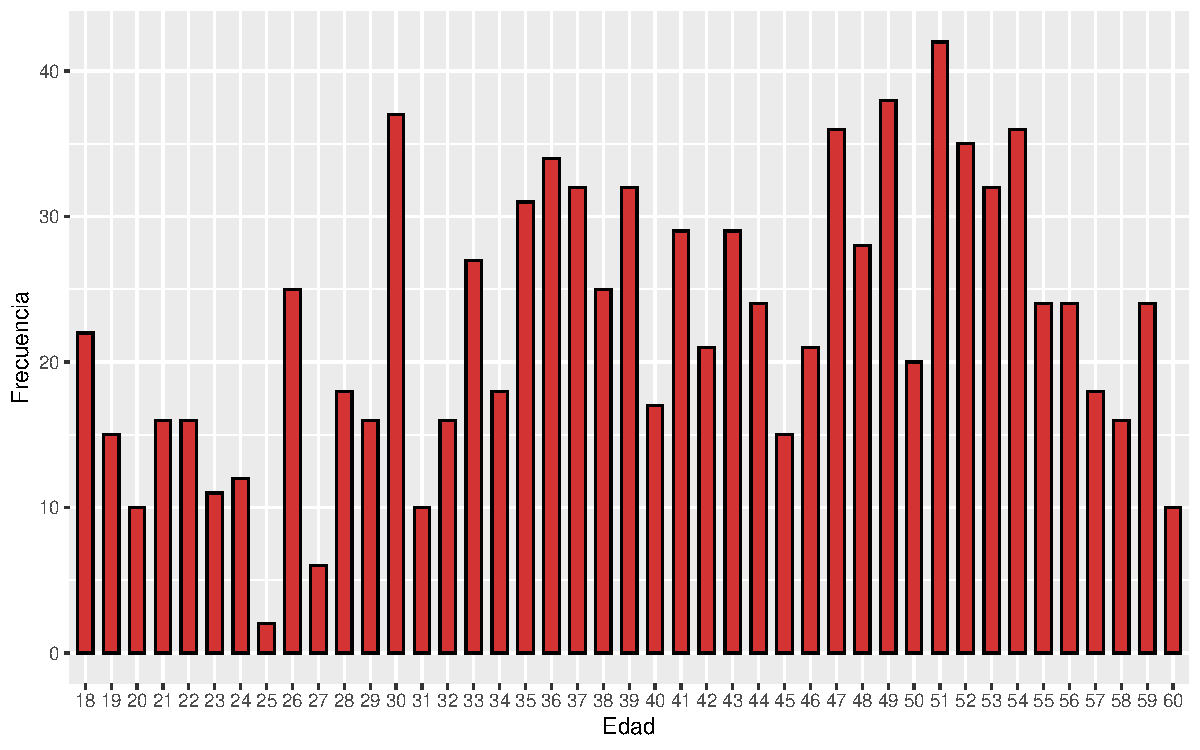
\includegraphics[width=\linewidth]{../../scripts/eda/eda_univar/char_age_distr.pdf}
    \caption[Distribución de los datos por edad]{Distribución de los datos según la edad real de los individuos. Se observa una mayor concentración de muestras en los rangos superiores a los 35 años.}
    \label{fig4:age}
\end{figure}
\begin{figure}[h]
    \centering
    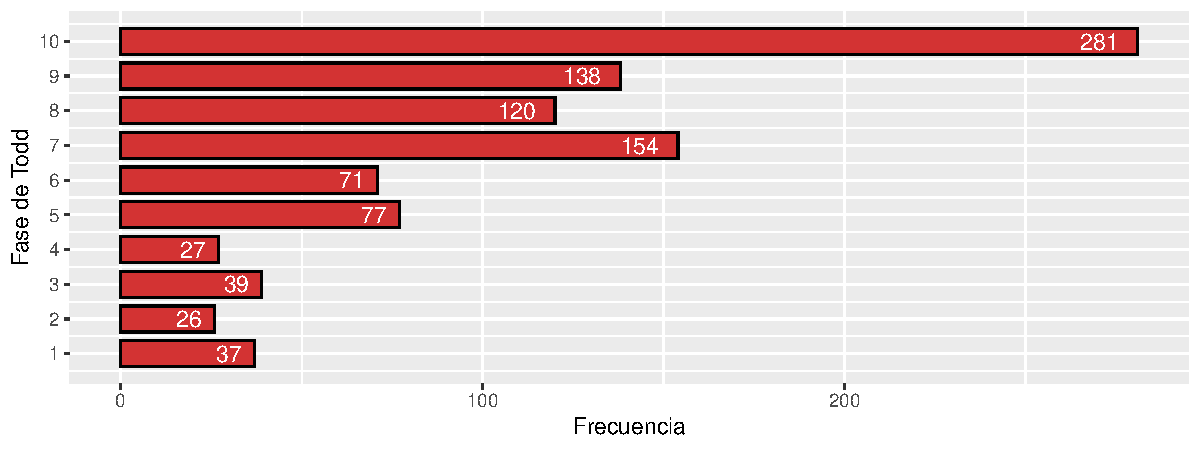
\includegraphics[width=\linewidth]{../../scripts/eda/eda_univar/char_t_phase_distr.pdf}
    \caption[Distribución de los datos por cada rango de edad]{Distribución de los datos por cada rango de edad del método de Todd. Se observa una mayor concentración de muestras entre las fases 7 y 10. Leyenda: \textbf{1}: 18-19 años, \textbf{2}: 20-21 años, \textbf{3}: 22-24 años, \textbf{4}: 25-26 años, \textbf{5}: 27-30 años, \textbf{6}: 30-35 años, \textbf{7}: 35-39 años, \textbf{8}: 39-44 años, \textbf{9}: 45-50 años, \textbf{10}: 50+ años.}
    \label{fig4:todd_phase}
\end{figure}

\subsection{Análisis Exploratorio de Datos}
\label{section4:data_eda}
Realizando un análisis exploratorio de los datos (\textit{Exploratory Data Analysis}, EDA), resulta de interés realizar una inspección visual preliminar de las mallas. En la Figura \ref{pb_3dexamples} se muestran tres mallas 3D de la sínfisis del pubis renderizados con iluminación fotorrealista desde tres ángulos diferentes relativos al lado relevante del hueso para los expertos, la cara sinfisaria o articular: vista lateral izquierda, frontal y lateral derecha. A partir de estas imágenes puede observarse que se trata de mallas 3D de alta complejidad geométrica y nivel de detalle. Además, al tratarse de estructuras anatómicas reales, presentan una alta variabilidad morfológica tanto en dimensiones como en proporciones, lo cual supone un reto adicional para los métodos de DL a aplicar.

Cabe destacar que el método seleccionado (ExMeshCNN, véase \ref{section4:methods}) no ha sido validado con datos de esta naturaleza, sino con conjuntos de datos sintéticos y de menor resolución. Aun así, se espera que su rendimiento se mantenga elevado, dado que está diseñado para capturar patrones discriminativos directamente desde la superficie de las mallas, independientemente de su nivel de complejidad o del origen biológico de las estructuras representadas.

Centrándose ahora en los datos asociados a cada malla, se observa que la muestra está compuesta por individuos de entre 18 y 60 años, cuya distribución se muestra en la Figura \ref{fig4:age}. Además, estos individuos han sido clasificados dentro de las 10 fases del método de Todd, tal como se aprecia en la Figura \ref{fig4:todd_phase}.

De ambos gráficos se aprecia que las edades más representadas corresponden a individuos de mayor edad, lo cual es coherente considerando el origen de los datos. Sin embargo, este patrón también evidencia un desbalance inherente en la muestra, un fenómeno esperado cuando se trabaja con datos reales.

\subsubsection{Análisis Univariable}
Continuando con el EDA enfocado en las nueve características del método de Todd, se observa un claro desbalance en la distribución de atributos, como se muestra en las gráficas correspondientes en las Figuras \ref{fig4:todd_chars_1}, \ref{fig4:todd_chars_2} y \ref{fig4:todd_chars_3}. Los atributos más representados son coherentes con las manifestaciones morfológicas que el hueso de la sínfisis del pubis presenta a edades más avanzadas.

Desde la perspectiva del balance de datos, las características USE (Subfigura \ref{fig4:todd_chars__use}), BN (Subfigura \ref{fig4:todd_chars__bn}), DP (Subfigura \ref{fig4:todd_chars__dp}) y LSE (Subfigura \ref{fig4:todd_chars__lse}) presentan un desbalance particularmente acentuado, con aproximadamente 95\%, 91\%, 90\% y 90\% de las muestras concentradas en un solo atributo, respectivamente. Este fuerte desbalance sugiere que estas características podrían tener un rendimiento limitado al ser utilizadas para el entrenamiento de modelos de DL.

\begin{figure}[p]
    \centering
    \begin{subfigure}{\textwidth}
        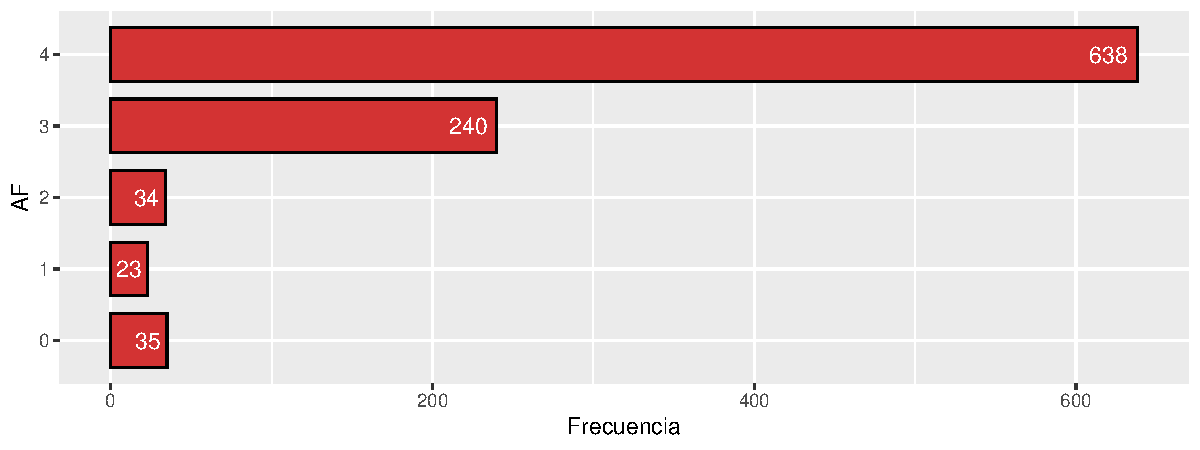
\includegraphics[width=\linewidth]{../../scripts/eda/eda_univar/char_af_distr.pdf}
        \caption{Característica AF. Leyenda: \textbf{0}: Porosidad Regular, \textbf{1}: Muy Definidas, \textbf{2}: Poco Profundas, \textbf{3}: Restos de Surcos, \textbf{4}: No hay surcos.}
        \label{fig4:todd_chars__af}
    \end{subfigure}

    \begin{subfigure}{\textwidth}
        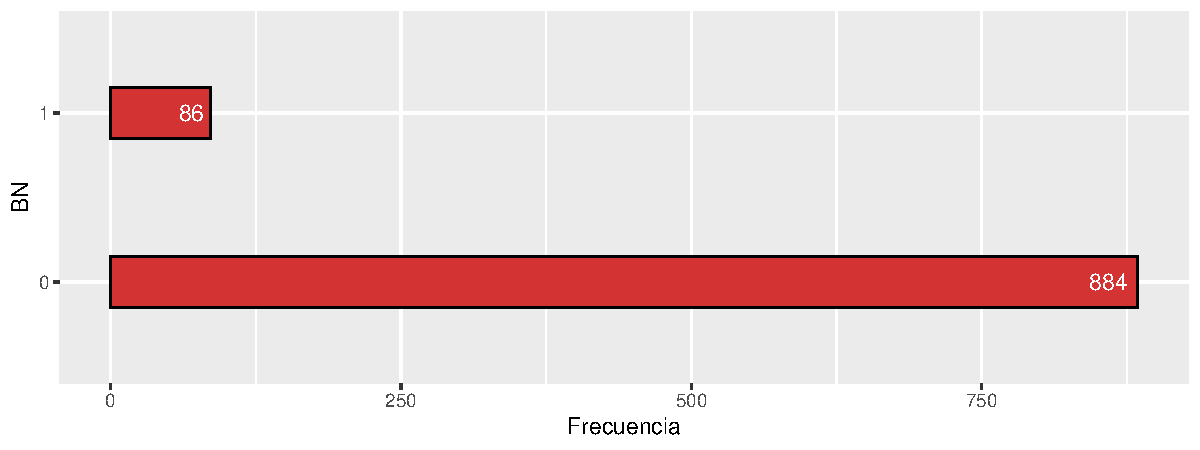
\includegraphics[width=\linewidth]{../../scripts/eda/eda_univar/char_bn_distr.pdf}
        \caption{Característica BN. Leyenda: \textbf{0}: Ausente, \textbf{1}: Presente.}
        \label{fig4:todd_chars__bn}
    \end{subfigure}
    
    \begin{subfigure}{\textwidth}
        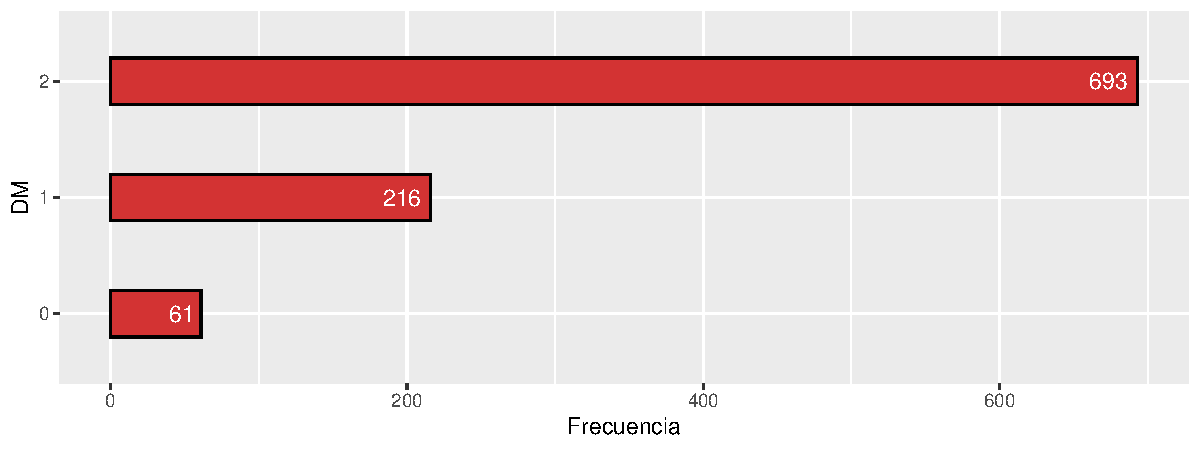
\includegraphics[width=\linewidth]{../../scripts/eda/eda_univar/char_dm_distr.pdf}
        \caption{Característica DM. Leyenda: \textbf{0}: No Definido, \textbf{1}: En Formación, \textbf{2}: Definido.}
        \label{fig4:todd_chars__dm}
    \end{subfigure}
    \caption[Distribución de las características de Todd (1 de 3)]{Distribución de las etiquetas para cada característica de Todd en el conjunto de datos (1 de 3). Para cada característica, se muestran las frecuencias de las diferentes clases observadas en los datos disponibles. Esta visualización permite apreciar el grado de desbalance entre clases y la variabilidad presente en cada rasgo morfológico.}
    \label{fig4:todd_chars_1}

\end{figure}
\begin{figure}[p]

    \begin{subfigure}{\textwidth}
        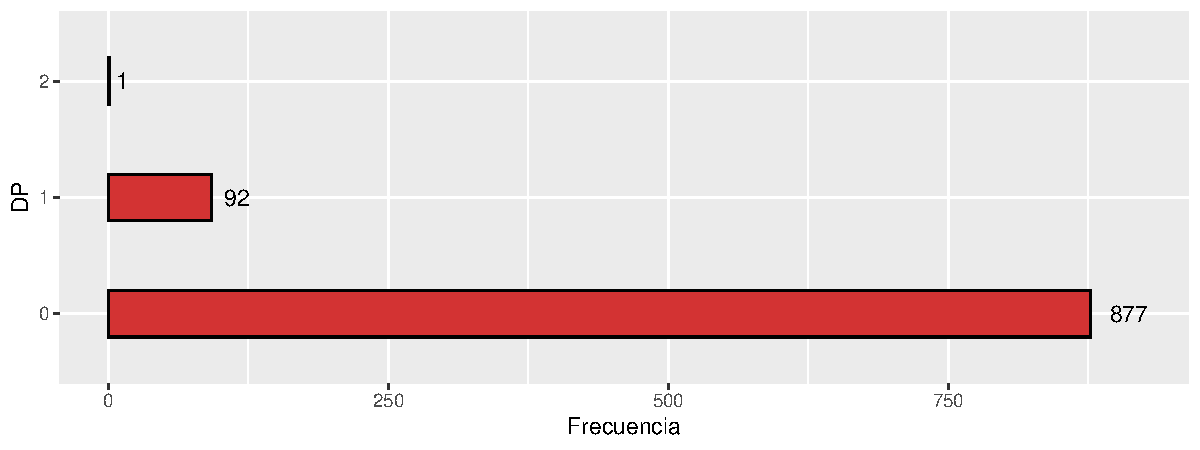
\includegraphics[width=\linewidth]{../../scripts/eda/eda_univar/char_dp_distr.pdf}
        \caption{Característica DP. Leyenda: \textbf{0}: Ausente, \textbf{1}: En Formación, \textbf{2}: Presente.}
        \label{fig4:todd_chars__dp}
    \end{subfigure}

    \begin{subfigure}{\textwidth}
        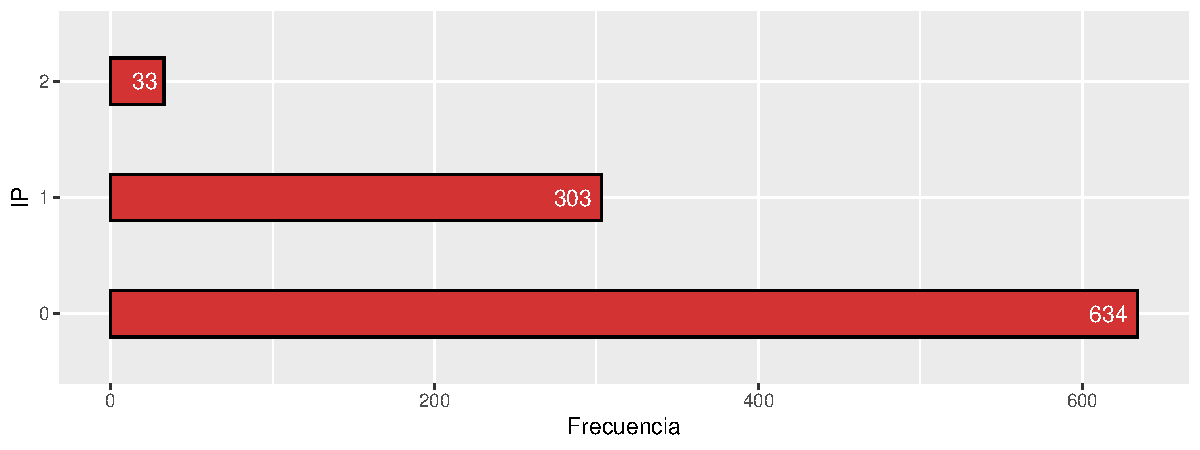
\includegraphics[width=\linewidth]{../../scripts/eda/eda_univar/char_ip_distr.pdf}
        \caption{Característica IP. Leyenda: \textbf{0}: No, \textbf{1}: Mediana, \textbf{2}: Sí.}
        \label{fig4:todd_chars__ip}
    \end{subfigure}

    \begin{subfigure}{\textwidth}
        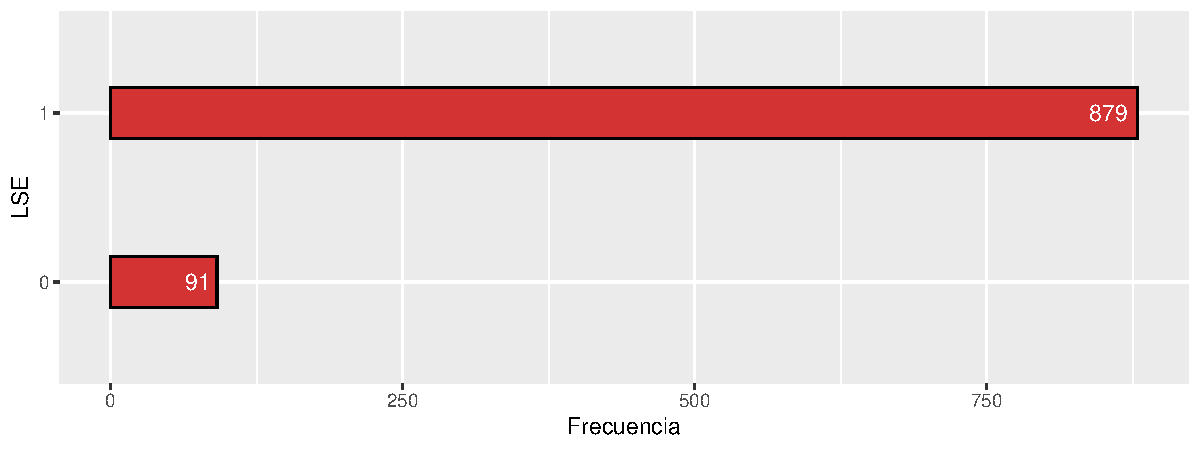
\includegraphics[width=\linewidth]{../../scripts/eda/eda_univar/char_lse_distr.pdf}
        \caption{Característica LSE. Leyenda: \textbf{0}: No Definido, \textbf{1}: Definido.}
        \label{fig4:todd_chars__lse}
    \end{subfigure}

    \caption[Distribución de las características de Todd (2 de 3)]{Distribución de las etiquetas para cada característica de Todd en el conjunto de datos (2 de 3). Para cada característica, se muestran las frecuencias de las diferentes clases observadas en los datos disponibles. Esta visualización permite apreciar el grado de desbalance entre clases y la variabilidad presente en cada rasgo morfológico.}
    \label{fig4:todd_chars_2}
\end{figure}
\begin{figure}[p]

    \begin{subfigure}{\textwidth}
        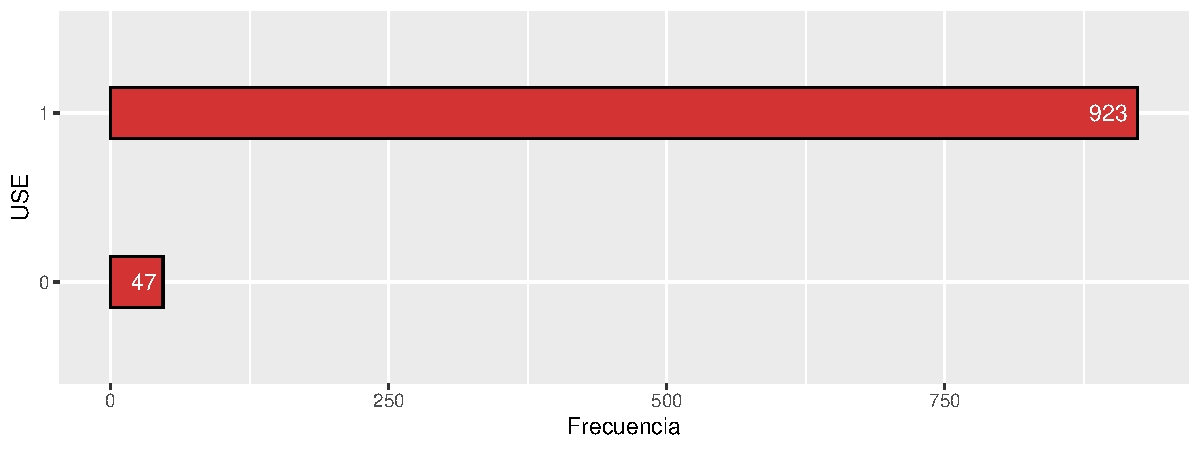
\includegraphics[width=\linewidth]{../../scripts/eda/eda_univar/char_use_distr.pdf}
        \caption{Característica USE. Leyenda: \textbf{0}: No Definido, \textbf{1}: Definido.}
        \label{fig4:todd_chars__use}
    \end{subfigure}

    \begin{subfigure}{\textwidth}
        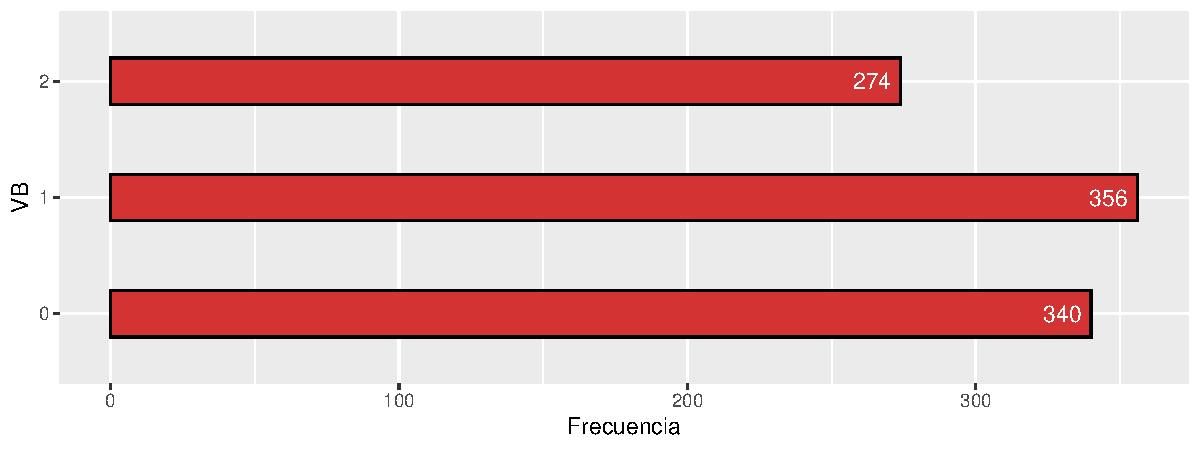
\includegraphics[width=\linewidth]{../../scripts/eda/eda_univar/char_vb_distr.pdf}
        \caption{Característica VB. Leyenda: \textbf{0}: Ausente, \textbf{1}: En Formación, \textbf{2}: Presente.}
        \label{fig4:todd_chars__vb}
    \end{subfigure}

    \begin{subfigure}{\textwidth}
        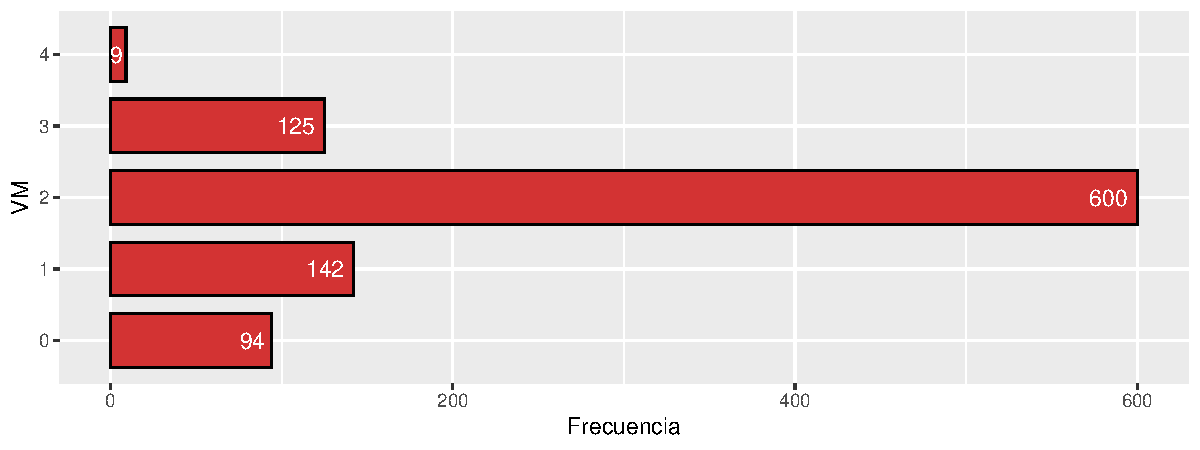
\includegraphics[width=\linewidth]{../../scripts/eda/eda_univar/char_vm_distr.pdf}
        \caption{Característica VM. Leyenda: \textbf{0}: Ausente, \textbf{1}: En Formación, \textbf{2}: Formado, Sin Excrecencias, \textbf{3}: Formado, Pocas Excrecencias, \textbf{4}: Formado, Muchas Excrecencias.}
        \label{fig4:todd_chars__vm}
    \end{subfigure}
    \caption[Distribución de las características de Todd (3 de 3)]{Distribución de las etiquetas para cada característica de Todd en el conjunto de datos (3 de 3). Para cada característica, se muestran las frecuencias de las diferentes clases observadas en los datos disponibles. Esta visualización permite apreciar el grado de desbalance entre clases y la variabilidad presente en cada rasgo morfológico.}
    \label{fig4:todd_chars_3}


\end{figure}

El resto de las características muestra un desbalance menos extremo, con entre el 60\% y el 70\% de los datos agrupados en una único atributo. La característica con mayor equilibrio en su distribución es el VB (Subfigura \ref{fig4:todd_chars__vb}), en la que los datos se reparten aproximadamente en un 33\% por atributo, dado que esta posee tres atributos distintos. Se espera que esta característica, junto con aquellas que presenten menos desbalance, proveerán mejores resultados al ser entrenadas por la red.

\subsubsection{Correlaciones}

\begin{figure}[p]
    \centering
    \begin{subfigure}{\textwidth}
        \centering
        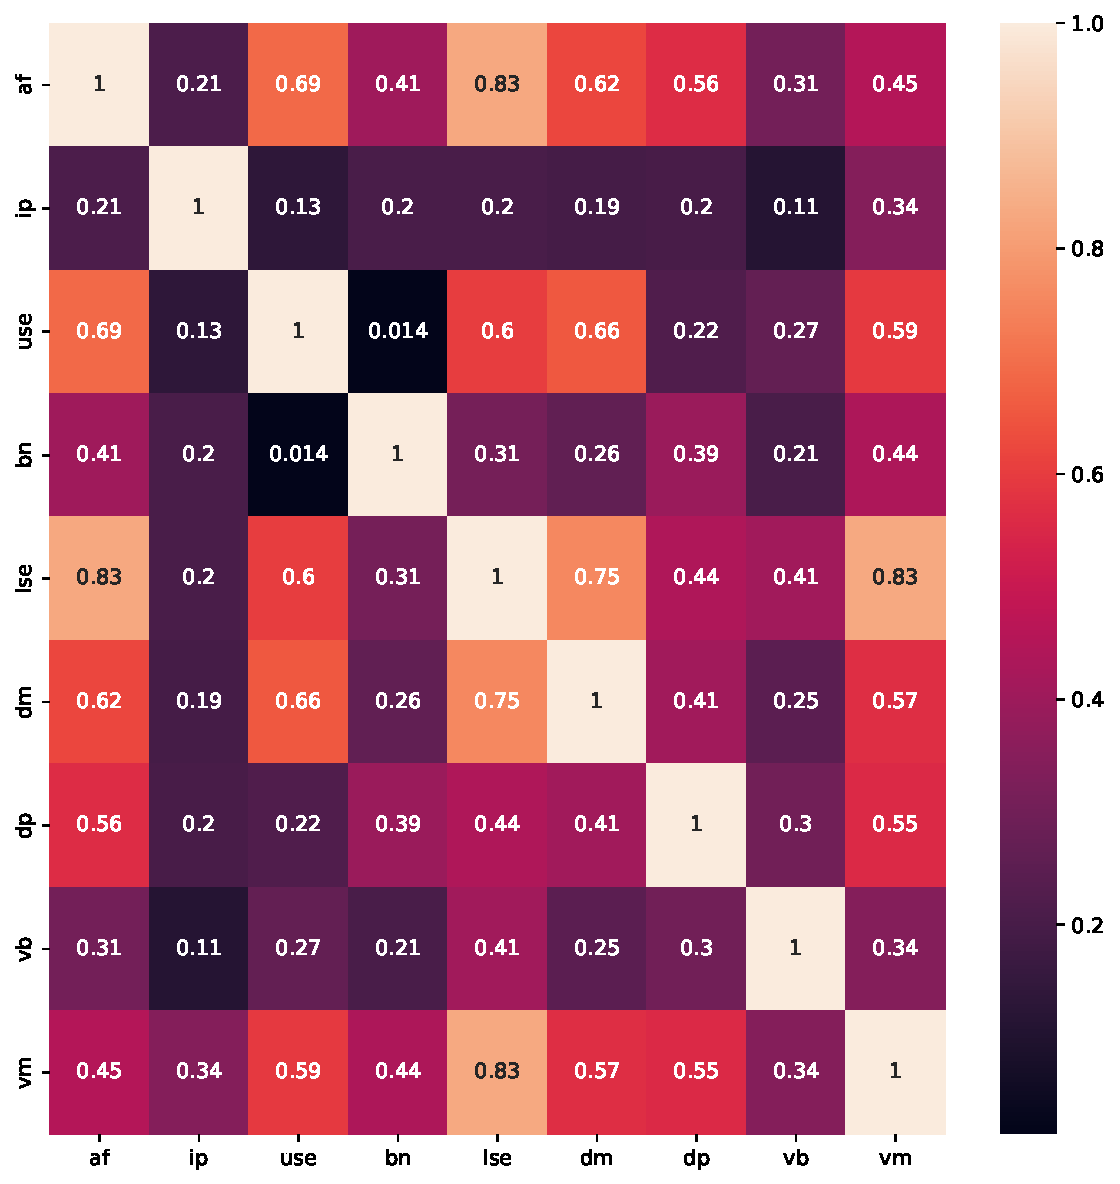
\includegraphics[width=0.6\linewidth]{../../scripts/eda/assoc_plot_cramersv.pdf}
        \caption{Mapa de calor de la V de Cramér}
        \label{fig4:todd_chars__cramersv}
    \end{subfigure}
    \begin{subfigure}{\textwidth}
        \centering
        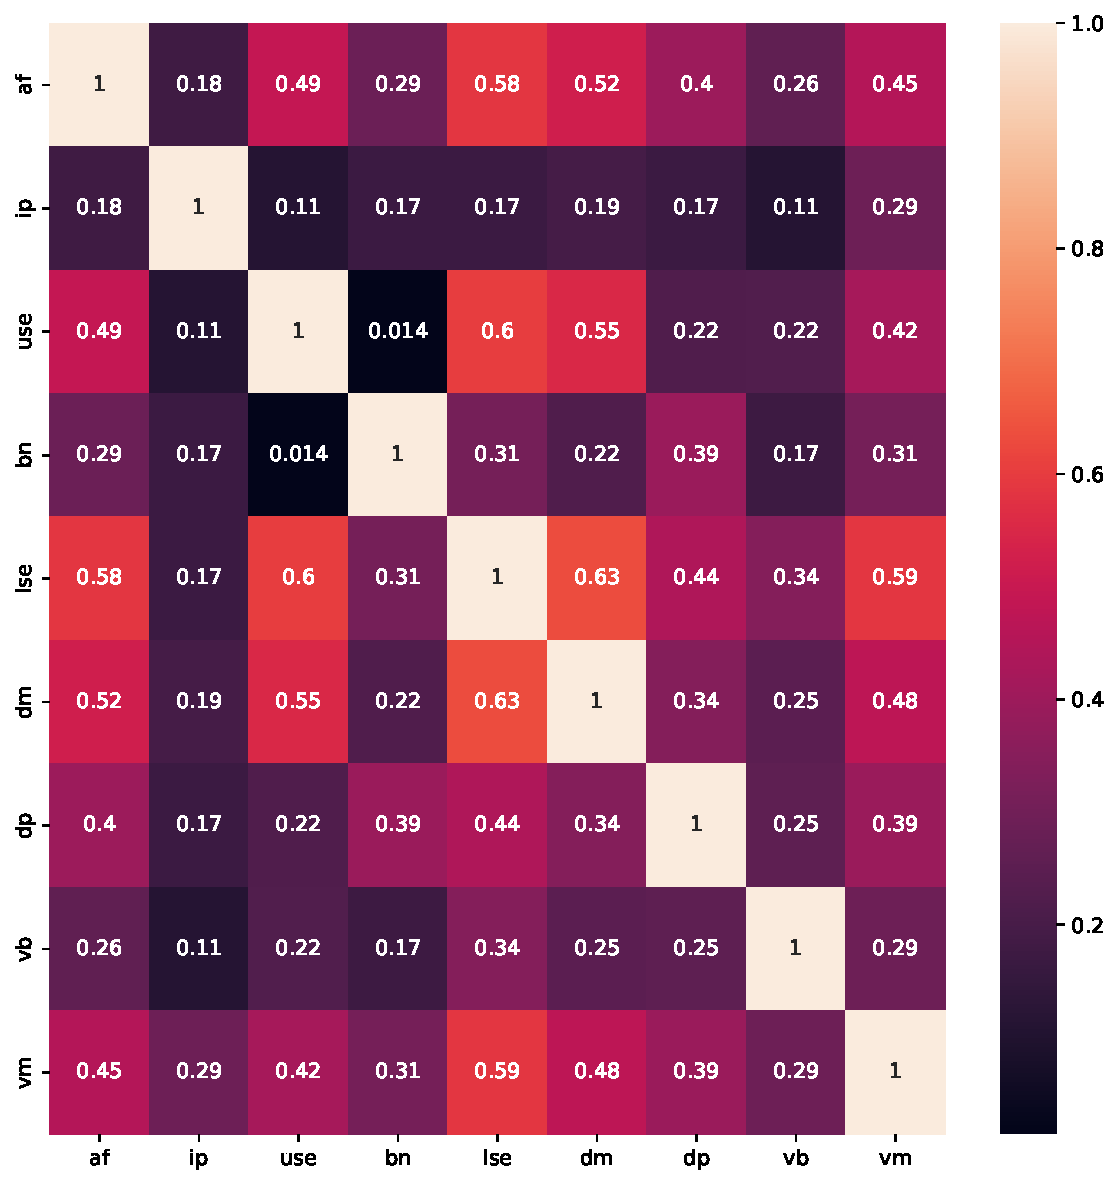
\includegraphics[width=0.6\linewidth]{../../scripts/eda/assoc_plot_tschuprow.pdf}
        \caption{Mapa de calor de la T de Tschuprow}
        \label{fig4:todd_chars__tschuprow}
    \end{subfigure}
    \caption[Mapas de calor de asociaciones entre características de Todd]{Mapas de calor que muestran las asociaciones entre las características de Todd utilizando la V de Cramér (a) y la T de Tschuprow (b). Los colores más claros indican asociaciones más fuertes entre pares de características. Los valores oscilan entre 0, lo que indica ausencia de asociación, y 1, que sugiere una asociación muy fuerte.}
    \label{fig4:todd_chars_correlogram}
\end{figure}

Si bien los datos empleados en este estudio no son de naturaleza tabular y se utilizan técnicas de DL que no requieren una extracción manual de características, resulta igualmente útil de cara a los experimentos, analizar las asociaciones existentes entre las nueve características del método de Todd. Dado que dichas variables son categóricas, se ha optado por emplear la V de Cramér \cite{sheskin_handbook_2020}, una medida estadística que cuantifica la intensidad de la asociación\footnote{Cabe destacar que la V de Cramér únicamente indica la presencia e intensidad de una relación entre variables, sin ofrecer información sobre la dirección de dicha asociación, esto a diferencia de las medidas de correlación para variables numéricas \cite{jimenez_nota_2024}.} entre dos variables categóricas. Un valor cercano a 1 indica una asociación fuerte entre ambas características, mientras que un valor próximo a 0 sugiere poca o ninguna asociación.

No obstante, la V de Cramér puede verse afectada por un sesgo cuando se aplica a tablas de contingencia no cuadradas, es decir, cuando el número de categorías en las variables comparadas es diferente, lo cual sucede en varias combinaciones de las características de Todd. Para corregir este efecto y obtener una interpretación más equilibrada del grado de asociación, se ha complementado el análisis con la T de Tschuprow, una medida alternativa que atenúa este sesgo y permite una comparación más justa entre pares de variables con distinta cardinalidad.

Se han generado mapas de calor por cada par de características, que pueden observarse en la Figura \ref{fig4:todd_chars_correlogram}, donde se aprecia que las asociaciones entre las características varían significativamente entre sí. Como era de esperarse, existen discrepancias ligeras entre los valores obtenidos mediante la V de Cramér y la T de Tschuprow. Para facilitar la interpretación de estos resultados, se ha incluido la Tabla \ref{table4:corr}, en la que se listan las tres características con mayor asociación para cada una.

Del análisis se concluye que las características LSE, AF y VM son, en general, las que presentan los mayores niveles de asociación con el resto, lo que sugiere una mayor dependencia entre ellas. En contraste, la característica IP muestra los niveles más bajos de asociación con las demás, seguida de BN, lo cual puede indicar un comportamiento más independiente. Este conocimiento será especialmente relevante en los experimentos de entrenamiento en modo multietiqueta, ya que incorporar características asociadas entre sí podría favorecer el aprendizaje del modelo y mejorar su rendimiento.

\begin{table}[t]
    \centering
    \begin{tabular}{|c|cc|}
        \hline
        \rowcolor[HTML]{D33333} 
        \cellcolor[HTML]{D33333}{\color[HTML]{FFFFFF} } & \multicolumn{2}{c|}{\cellcolor[HTML]{D33333}{\color[HTML]{FFFFFF} Características con mayor asociación}} \\ \cline{2-3} 
        \rowcolor[HTML]{D33333} 
        \multirow{-2}{*}{\cellcolor[HTML]{D33333}{\color[HTML]{FFFFFF} Característica}} & \multicolumn{1}{c|}{\cellcolor[HTML]{D33333}{\color[HTML]{FFFFFF} V de Cramér}} & {\color[HTML]{FFFFFF} T de Tschuprow} \\ \hline
        AF & \multicolumn{2}{c|}{DM, LSE, USE} \\ \cline{2-3} 
        BN & \multicolumn{1}{c|}{AF, DP, VM} & DP, LSE, VM \\ \cline{2-3} 
        DM & \multicolumn{2}{c|}{AF, LSE, USE} \\ \cline{2-3} 
        DP & \multicolumn{1}{c|}{AF, LSE, VM} & AF, BN, LSE \\
        IP & \multicolumn{1}{c|}{AF, LSE, VM} & AF, DM, VM \\
        LSE & \multicolumn{1}{c|}{AF, DM, VM} & DM, USE, VM \\ \cline{2-3} 
        USE & \multicolumn{2}{c|}{AF, DM, LSE} \\ \cline{2-3} 
        VB & \multicolumn{2}{c|}{AF, LSE, VM} \\ \cline{2-3} 
        VM & \multicolumn{1}{c|}{DM, LSE, USE} & AF, DM, LSE \\ \hline
    \end{tabular}
    \caption[Cuadro resumen de las asociaciones más fuertes entre características de Todd]{Resumen de las asociaciones más fuertes entre cada característica del método de Todd, calculadas mediante la V de Cramér y la T de Tschuprow. Para cada característica, se presentan las tres características con mayor grado de asociación. Se observa que, en algunos casos, ambos coeficientes identifican las mismas características asociadas, mientras que en otros difieren, lo que resalta la sensibilidad de cada medida frente a la estructura de las variables categóricas.}
    \label{table4:corr}
\end{table}

\subsubsection{Preparación de los datos}
\label{section4:data_preparation}
De la muestra original de 497 individuos, es decir, un total de 986 huesos correspondientes a las sínfisis del pubis izquierda y derecha, fue necesario eliminar 16 muestras por diversos motivos: presencia de deformidades anatómicas, ausencia del archivo OBJ asociado o falta de correspondencia entre el modelo 3D y los datos etiquetados provistos. Se opta por utilizar las 970 muestras restantes en su totalidad (484 huesos izquierdos y 486 derechos), ya que en problemas de DL es fundamental contar con un volumen de datos considerable, aunque estos estén altamente desbalanceados, pues se pueden utilizar diversas técnicas para mitigar el efecto que produce esto al rendimiento de un modelo. 

Cabe destacar que, en el caso de la característica DP (Subfigura \ref{fig4:todd_chars__dp}), el atributo 3 (\say{Presente}) cuenta con solo una muestra, lo cual impide que el modelo pueda aprender representaciones significativas para dicho atributo. Por tanto, esta muestra será eliminada durante el entrenamiento de modelos de DL que hagan uso de dicha característica. Además, el atributo 2 originalmente denominado \say{En Formación} será renombrado a \say{Presente}, con el objetivo de mantener la consistencia semántica.

Las 970 mallas presentan una resolución media de 994,601 triángulos, con un mínimo de 329,438 y un máximo de 1,688,348 triángulos. Para poder aplicar el método ExMeshCNN, descrito en la Sección \ref{section4:methods}, es necesario que todas las mallas tengan una resolución uniforme. Una opción inicial considerada fue remuestrear las mallas al número medio de triángulos; sin embargo, este tamaño resulta inviable computacionalmente con el hardware disponible.

Por esta razón, se ha procedido a reducir la resolución de las mallas a 100,000, 50,000 y 25,000 triángulos, utilizando las técnicas descritas en la Sección \ref{section4:data_reduction}. La elección de 100,000 triángulos responde al objetivo de mantener la mayor fidelidad geométrica posible sin que ello comprometa la viabilidad computacional de los entrenamientos. Tal como se demuestra en los experimentos de la Sección \ref{section5:experiment_edge_collapse}, esta reducción no afecta significativamente la fidelidad topológica de las mallas originales. Las resoluciones de 50,000 y 25,000 triángulos se han incluido para analizar cómo afectan reducciones más agresivas al rendimiento del modelo. La comparación mediante la distancia de Hausdorff indica que las diferencias geométricas respecto al modelo original son, en general, mínimas. Esto sugiere que incluso con resoluciones inferiores, las mallas conservan en buena medida la información morfológica necesaria para los experimentos, haciendo viable su uso en tareas de clasificación sin una pérdida drástica de calidad.

Adicionalmente, el método requiere que las mallas posean una geometría y topología correctas. Dado que estas mallas provienen de escaneos de objetos anatómicos reales, es esperable que algunas presenten incompletitud o defectos estructurales, lo que impide su uso directo con ExMeshCNN. Para solventar estos problemas, se aplicaron técnicas de reparación y sellado descritas en la Sección \ref{section4:data_repair}, con el objetivo de restaurar la geometría y garantizar la integridad topológica de cada modelo antes de ser procesado por la red neuronal.

\section{Métodos}
\label{section4:methods}
Como se ha mencionado previamente en la Sección \ref{section3:meshes}, ExMeshCNN \cite{kim_exmeshcnn_2022} representa el estado del arte en el procesamiento de mallas poligonales mediante DL y por lo tanto ha sido el método elegido para realizar los experimentos. A continuación se describe de qué forma el \textit{framework} adapta los datos para poder ser utilizados con convoluciones.

\subsection{Capa de descriptores}
Las representaciones en cuadrícula, como en el caso de imágenes, resultan convenientes porque encapsulan tanto la información de conectividad (es decir, la vecindad local entre píxeles) como las características asociadas (como los valores RGB) en una única estructura matricial. Sin embargo, esta estrategia no puede trasladarse directamente a las mallas tridimensionales debido a su naturaleza irregular y a la ausencia de un orden canónico entre sus elementos.

Para abordar esta limitación, se introducen dos capas iniciales en la red, denominadas \say{descriptores}, cuyo propósito es extraer de la malla información que permita caracterizar cada cara triangular, de forma de que sea invariante e independientemente del orden en el que se encuentran. De esta forma se obtiene información que es similar a los valores RGB de un píxel, y a los cuales se les puede aplicar convoluciones permitiendo que el modelo pueda aprender efectivamente partiendo de una estructura 3D sin representación regular. 

\subsubsection{Descriptor geodésico basado en aristas}
El objetivo de este descriptor es capturar características geodésicas locales asociadas a los triángulos de la malla, características que han sido mayoritariamente ignoradas en la literatura actual. Se parte del concepto de distancia geodésica entre caras, definida como el camino más corto a través de aristas que conecta el centro de un triángulo objetivo con un vértice de un triángulo adyacente, pasando por uno de los vértices del triángulo objetivo. No obstante, en mallas triangulares esta métrica resulta limitada, ya que la cantidad de aristas involucradas en dichos caminos es siempre dos, lo cual no aporta mucha información.

Para enriquecer esta representación, se incorporan ideas provenientes de la convolución geodésica propuesta por Schult et al. \cite{schult_dualconvmesh-net_2020}, que toma en cuenta no solo la longitud del camino, sino también su curvatura. De este modo, dos caminos con la misma longitud, pero distinta curvatura permiten ser diferenciados.

Sin embargo, dicha convolución geodésica presenta una limitación importante: la ambigüedad en el orden de los caminos posibles. Dado que estos no poseen una estructura de vecindad ordenada, una misma operación de convolución puede producir diferentes resultados dependiendo del orden de los elementos procesados, comprometiendo así la consistencia del aprendizaje.

Partiendo de estas ideas, se propone el siguiente descriptor $\mathcal{K}$, definido en la Ecuación \ref{eq4:geodesic}:
\begin{equation}
\label{eq4:geodesic}
    \mathcal{K}
(\bar{\textbf{a}_{t}}) = \theta_{0} \sum_{j}^{3} \textbf{u}_{t}^{j} + \theta_{1} \sum_{j}^{3}  \overrightarrow{\textbf{n}}_{t}^{j} + \theta_{2} \sum_{j}^{3} |\textbf{e}_{n(t)}^{j,1} - \textbf{e}_{n(t)}^{j,2}|
\end{equation}
Donde: 
\begin{itemize}
    \item $\bar{\textbf{a}_{t}}$ representa el conjunto conformado por un triángulo objetivo $f_{t}$ y sus tres triángulos vecinos topológicos $f_{n(t)_j}$, con $j \in \left\{1,2,3\right\}$.
    \item $\textbf{u}_{t}^{j}$ describe el vector entre el centro del triángulo $\textbf{c}_t$ y el vértice $j$-ésimo $\textbf{v}_{t}^j$ definido como  $\textbf{u}_{t}^{j} = \textbf{c}_t - \textbf{v}_t^j$ con $j \in \left\{1,2,3\right\}$.
    \item $\overrightarrow{\textbf{n}}_{t}^{j}$ es la normal del vértice $\textbf{v}_t^j$, calculada como la media de las normales de los triángulos que rodean dicho vértice.
    \item $\textbf{e}_{n(t)}^{j,k}$ representa la arista entre el vértice $\textbf{v}_{t}^j$ del triángulo objetivo y un vértice $\textbf{v}_{n(t)}^{j,k}$ del triángulo vecino, donde $k \in \left\{1,2\right\}$. Dado que solo existen dos caminos posibles desde un vértice $\textbf{v}_t^j$ hacia vértices de triángulos vecinos a través de una arista común, la diferencia $|\textbf{e}_{n(t)}^{j,1} - \textbf{e}_{n(t)}^{j,2}|$ captura una característica invariante al orden debido al valor absoluto.
    \item Los términos $\theta_0, \theta_1 $ y $\theta_2$ son parámetros entrenables por la red.
\end{itemize}


\begin{figure}
    \centering
    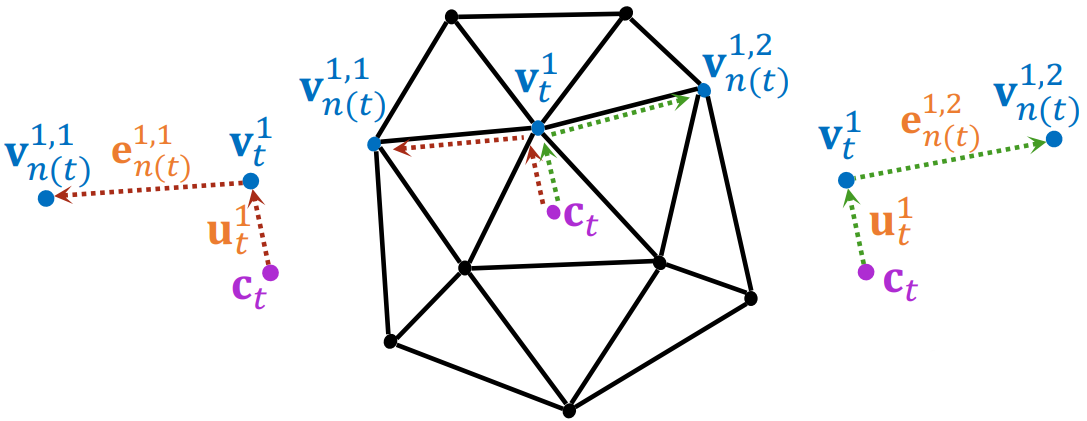
\includegraphics[width=\linewidth]{figures/4_materials-methods/geodesic_descriptor.png}
    \caption[Ejemplo visual del descriptor geodésico]{Ejemplo visual del descriptor geodésico, donde se toma como triángulo objetivo $f_t$ el que se encuentra en el centro de la malla. Se observa el vector $\textbf{u}_{t}^{1}$ que conecta el centro del triángulo $\textbf{c}_t$ con uno de sus vértices, $\textbf{v}_t^1$, así como las aristas $\textbf{e}_{n(t)}^{1,1}$ (izquierda) y $\textbf{e}_{n(t)}^{1,2}$ (derecha), que enlazan el triángulo $f_t$ con sus triángulos vecinos a través del vértice $\textbf{v}_t^1$. Este proceso se repite de forma análoga para los otros dos vértices del triángulo objetivo.}
    \label{geod_descrp}
\end{figure}

Para una mejor comprensión de estos términos, se recomienda consultar la Figura \ref{geod_descrp}. En esencia, lo que se realiza es un mapeo del triángulo objetivo y su vecindario topológico a un espacio de características geodésicas capturando las siguientes propiedades:
\begin{itemize}
    \item Forma local del triángulo, mediante el término $\textbf{u}_{t}^{j}$, que describe cómo se distribuyen espacialmente los vértices con respecto al centroide.
    \item Orientación local, reflejada en $\overrightarrow{\textbf{n}}_{t}^{j}$, que aporta información sobre la dirección normal de la superficie.
    \item Relaciones geodésicas entre triángulos vecinos, a través del término $|\textbf{e}_{n(t)}^{j,1} - \textbf{e}_{n(t)}^{j,2}|$, que captura la variación entre las conexiones posibles.
\end{itemize}

Además, el descriptor actúa funcionalmente como un filtro de convolución 1D de tamaño 3, ya que posee parámetros entrenables. Esto permite realizar subsiguientes convoluciones 1D sobre el vector de características obtenido.

\FloatBarrier

\subsubsection{Descriptor geométrico basado en caras}
En la literatura, las características geométricas más comúnmente empleadas para describir las caras triangulares incluyen el vector normal de la misma, su centroide y el ángulo que forma con las caras vecinas. Dado que estas características son de bajo nivel y, en cierta medida, de naturaleza heurística, se propone el descriptor $\mathcal{G}$, definido en la Ecuación \ref{eq4:geometric}, con el objetivo de capturar representaciones de alto nivel que integren dicha información geométrica.

\begin{equation}
\label{eq4:geometric}
    \mathcal{G}(\bar{\textbf{a}_{t}}) = \phi_{0} \textbf{c}_{t} + \phi_{1} \overrightarrow{\textbf{n}}_{t} + \phi_{2} \sum_{j}^{3} | \textbf{c}_{t} - \textbf{c}_{n(t)}^{j} | + \phi_{3} \sum_{j}^{3} | \overrightarrow{\textbf{n}}_{t} \times \overrightarrow{\textbf{n}}_{n(t)}^j |
\end{equation}
Donde:
\begin{itemize}
    \item Los términos $\textbf{c}_{t}$ y $\overrightarrow{\textbf{n}}_{t}$ capturan la información relativa a la posición y orientación de la cara triangular $f_t$ en el espacio.
    \item Los términos $| \textbf{c}_{t} - \textbf{c}_{n(t)}^{j} |$ y $| \overrightarrow{\textbf{n}}_{t} \times \overrightarrow{\textbf{n}}_{n(t)}^j |$ capturan la relación que tiene el triángulo objetivo con su vecindario local respecto a la distancia entre sí y el ángulo que forman.
    \item Los términos $\phi_{0}, \phi_{1}, \phi_{2} $ y $\phi_{3}$ son parámetros entrenables por la red.
\end{itemize}

De esta forma, se logra realizar otro mapeo de las caras triangulares junto a su vecindario topológico a un espacio de características geométricas y, al igual que sucede con el descriptor de aristas, se tiene esencialmente una capa entrenable por la red y que su resultado es factible realizarle convoluciones 1D. La Figura \ref{geom_descrp} permite visualizar estos conceptos de forma clara.

\begin{figure}[htb]
    \centering
    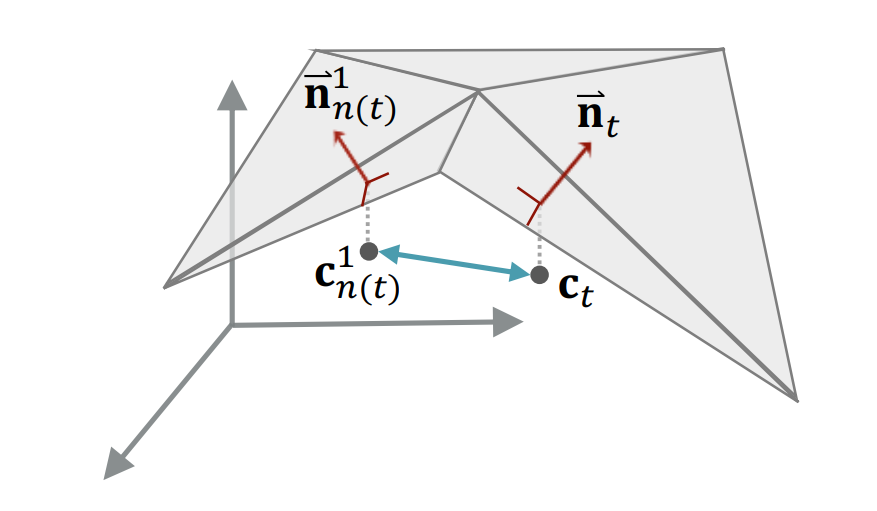
\includegraphics[width=0.75\linewidth]{figures/4_materials-methods/geometric_decriptor.png}
    \caption[Ejemplo visual del descriptor geométrico]{Ejemplo visual del descriptor geométrico, donde se muestra el triángulo objetivo $f_t$ (a la derecha de la malla) junto con su vecino topológico $f_{n(t)_1}$. Se destacan los centroides de ambos triángulos, $\textbf{c}_{t}$ y $ \textbf{c}_{n(t)}^{1}$, utilizados para calcular el vector $\left| \textbf{c}_{t} - \textbf{c}_{n(t)}^{1} \right|$, representado en azul en la figura. También se visualizan sus normales respectivas, $\overrightarrow{\textbf{n}}_{t}$ y $\overrightarrow{\textbf{n}}_{n(t)}^{1}$, cuya relación angular se captura mediante su producto cruzado.}
    \label{geom_descrp}
\end{figure}


En resumen, la primera capa de cualquier red construida con ExMeshCNN se compone de los dos descriptores $\mathcal{K}(\bar{\textbf{a}}_t)$ y $\mathcal{G}(\bar{\textbf{a}}_t)$, que funcionalmente actúan como capas convolucionales 1D pues poseen parámetros entrenables, pero que están realizando un mapeo de cada triángulo a un espacio de características geométricas y geodésicas. El resultado de los descriptores es concatenado como se observa en la Ecuación \ref{eq4:concat} para ser utilizado por las capas verdaderamente convolucionales.
\begin{equation}
    \label{eq4:concat}
    \mathcal{F}_{t} = \left[\mathcal{K}(\bar{\textbf{a}}), \mathcal{G}(\bar{\textbf{a}}) \right]
\end{equation}
Donde $\mathcal{F}_{t}$ es el vector de características de cada cara triangular. Para que estos descriptores funcionen correctamente, es necesario que las mallas posean una geometría y topología correctas: esto garantiza que una cara triangular siempre tendrá 3 vecinos a su alrededor, un requisito necesario para poder realizar el mapeo entre las caras triangulares y las características extraídas por los descriptores. 

\FloatBarrier
\subsection{Capas convolucionales}
Dado que las mallas no poseen un orden canónico en sus triángulos, es necesario realizar un preprocesamiento antes de aplicar una operación de convolución 1D. Para ello, se expande el vector de características de cada triángulo $f_i$ de la siguiente manera:
\begin{align}
    \alpha_i &= \mathcal{F}_{i} \\
    \beta_i &= \sum_{j}^{3} | \mathcal{F}_{i} - \mathcal{F}_{n(i)}^{j}| 
\end{align}
Donde:
\begin{itemize}
    \item $\alpha_i$ representa las características propias del triángulo $f_i$.
    \item $\beta_i$ representa un agregado de las diferencias absolutas entre las características de $f_i$ y las de sus tres triángulos vecinos topológicos $f_{n(i)}^{j}$, con $j \in {1, 2, 3}$.
\end{itemize}

Este paso expande temporalmente el conjunto de datos, duplicando la cantidad de triángulos al generar dos entradas por triángulo: $\alpha_i$ y $\beta_i$. Posteriormente, se aplica una convolución 1D con un kernel de tamaño 2 y un \textit{stride} de 2. Esta configuración permite que cada operación de convolución combine la información de $\alpha_i$ y $\beta_i$, de manera que la operación es invariante al orden de los triángulos en la malla. Al mismo tiempo, el uso de \textit{stride} 2 permite recuperar la dimensionalidad original del conjunto de datos.

A diferencia de otros enfoques, ExMeshCNN mantiene fijo el tamaño del filtro de convolución entre capas y controla la capacidad de la red a través de la densidad (profundidad) de las mismas. Se toma esta decisión debido a que facilita el uso de técnicas de interpretabilidad como Grad-CAM, permitiendo identificar directamente qué triángulos de las mallas contribuyen al resultado final del modelo de forma equivalente a como se haría con un píxel en una imagen: Se observa el flujo de los gradientes en la última capa convolucional y se colorean los triángulos a base de su influencia en la clasificación que ha realizado la red. Por esto se necesita que las mallas 3D posean un número idéntico y fijo de triángulos para poder ser procesadas por ExMeshCNN.

\subsection{ExMeshCNN vs MeshCNN}
\label{exmeshcnn_vs_meshcnn}

\begin{table}[h]
    \centering
    \begin{tabular}{|p{0.3\linewidth}|p{0.3\linewidth}|p{0.3\linewidth}|}
    \hline
    \rowcolor[HTML]{D33333} 
    {\color[HTML]{FFFFFF} \textbf{Característica}} & {\color[HTML]{FFFFFF} \textbf{MeshCNN}} & {\color[HTML]{FFFFFF} \textbf{ExMeshCNN}} \\ \hline
    Equivalencia al píxel & Aristas & Caras y aristas \\ \hline
    Equivalencia a canales RGB & Vector heurístico de 5 componentes geométricas. & Vector conformado por salida de descriptores geométrico y geodésico. \\ \hline
    Convolución & Convolución 2D sobre aristas. & Convolución 1D sobre vector de características obtenida de los descriptores. \\ \hline
    \textit{Pooling} & Por colapso de aristas adaptativo. & Solo utilizado para conectar la parte convolucional con parte totalmente conectada de la red. \\ \hline
    Explicabilidad & Por \textit{pooling}, se retiene el detalle luego de cada operación de \textit{pooling} en las regiones de interés al modelo. & Por Grad-CAM adaptado para aplicarse a los triángulos con más respuesta en las convoluciones 1D. \\ \hline
    \end{tabular}
    \caption[Resumen de las diferencias entre MeshCNN y ExMeshCNN]{Resumen de las diferencias principales entre MeshCNN y ExMeshCNN.}
    \label{meshcnn_vs_exmeshcnn}
\end{table}

Aunque su nombre podría sugerir que se trata de una simple extensión de MeshCNN, el enfoque ExMeshCNN difiere de forma sustancial respecto a dicho \textit{framework}, el cual fue utilizado en el TFG predecesor a este trabajo, cuando aún representaba el estado del arte en el procesamiento de mallas mediante técnicas de DL. En la Tabla \ref{meshcnn_vs_exmeshcnn} se observa un resumen de las diferencias entre los \textit{frameworks}, las cuales son detalladas a continuación.

En cuanto a la operación de convolución, MeshCNN la aplica directamente sobre las aristas de una malla, utilizando un vector de cinco componentes que representan características exclusivamente geométricas y, en su mayoría, de naturaleza heurística: ángulos diedros entre los dos triángulos que comparten una arista, ángulos internos perpendiculares a la arista, y la relación entre la longitud de la arista y la longitud perpendicular de los triángulos. Este vector puede considerarse análogo a los valores RGB de un píxel en una imagen en el contexto de una CNN 2D tradicional.

Por el contrario, ExMeshCNN realiza convoluciones 1D sobre vectores de características extraídas a partir de descriptores geométricos y geodésicos definidos sobre las caras y aristas de la malla. Estos descriptores se calculan de manera sistemática al inicio de cada red definida con ExMeshCNN y constituyen el equivalente a la información de entrada (como los valores RGB) que una red convolucional necesita. A diferencia de MeshCNN, estas características no son heurísticas, sino que derivan de propiedades matemáticas bien definidas de la geometría y topología de la malla, proporcionando mayor capacidad de generalización. Además, al ser tratadas como entradas parametrizables, la red puede aprender durante el entrenamiento a atenuar o enfatizar aquellas características que resulten más relevantes para la tarea específica. ExMeshCNN transforma el problema tridimensional de procesado de mallas en un problema adaptable a convoluciones 1D, gracias al mapeo estructurado que realizan sus descriptores. Esto permite un tratamiento más flexible, explicable y rico en información que el enfoque tradicional propuesto por MeshCNN.

MeshCNN introduce operaciones de \textit{pooling} adaptativo mediante el colapso de aristas, que pueden aplicarse entre capas convolucionales para reducir progresivamente la fidelidad de las mallas. El objetivo principal de este mecanismo es doble: por un lado, emular el efecto de concentración de información que ofrece el \textit{pooling} en CNNs tradicionales 2D, y por otro, proporcionar un cierto nivel de explicabilidad al modelo: al observar las regiones de la malla que retienen mayor detalle, se puede inferir en qué se está centrando la red para llevar a cabo su tarea. Si bien este enfoque es lógico, presenta ciertas limitaciones prácticas. En particular, comparar visualmente las mallas originales con sus versiones reducidas puede resultar complejo, especialmente cuando las mallas presentan formas irregulares. En tales casos, la información obtenida puede no ser lo suficientemente clara o interpretativa como para brindar una explicabilidad efectiva.

En contraste, ExMeshCNN no incorpora operaciones de \textit{pooling} estructural en el diseño de sus arquitecturas. El \textit{pooling} se limita a su uso tradicional como nexo entre la parte convolucional y la parte totalmente conectada de la red. En su lugar, se opta por el uso de una adaptación del método Grad-CAM, aprovechando que las redes generadas utilizan convoluciones 1D nativas. Esta decisión aporta una ventaja clara en términos de interpretabilidad: Grad-CAM permite visualizar directamente sobre la malla original las regiones más relevantes para la predicción del modelo, sin necesidad de comparar diferentes versiones de la misma. Además, al ser una técnica bien establecida y ampliamente utilizada, facilita el análisis y la presentación de resultados de forma más intuitiva y directa.

Finalmente, el uso de convoluciones 1D nativas en ExMeshCNN, en lugar de adaptaciones de convoluciones 2D como en MeshCNN, aporta una ventaja significativa en términos de eficiencia computacional. Esta mayor eficiencia permite llevar a cabo un mayor número de experimentos y pruebas en menos tiempo, lo que resulta especialmente valioso en entornos de investigación donde los recursos computacionales y el tiempo de entrenamiento son factores limitantes.
    
   %  % Experimentos
    \chapter{Experimentos}

\section{Implementación}
\label{section4:implementation}
\subsection{Entorno de desarrollo}
\subsubsection{Software}
Debido a su amplio uso en el ámbito de la IA y la Ciencia de Datos, y siendo el lenguaje de programación utilizado para la implementación de ExMeshCNN, este TFM ha sido desarrollado íntegramente en Python 3. Para la construcción de las redes neuronales se ha empleado de forma predominante la librería PyTorch junto con la librería de optimización de parámetros Optuna, complementada por otras bibliotecas ampliamente utilizadas en ML como NumPy, SciPy, Scikit-Learn y Pandas.

Dado que los datos tratados son de naturaleza tridimensional, se ha recurrido extensivamente a herramientas especializadas para la manipulación de mallas 3D. Entre ellas destacan el software de código abierto Blender y su API para Python, así como las librerías PyMeshLab, Trimesh y OpenMesh.

La gestión del control de versiones se ha llevado a cabo mediante Git y GitHub. Por otro lado, la gestión de dependencias del entorno Python se ha realizado mediante un entorno virtual (\textit{Virtual Environment}) específico para este proyecto.

El código desarrollado en el presente trabajo se encuentra disponible en el siguiente repositorio: \url{https://github.com/RhinoBlindado/datcom-tfm}.

\subsubsection{Hardware}
La ejecución de este TFM se ha llevado a cabo en dos entornos diferenciados: uno local y otro remoto.

El entorno local consistió en un ordenador portátil Asus FX505DT equipado con un procesador AMD Ryzen 7 3750H, 16 GB de memoria RAM y una GPU Nvidia GeForce GTX 1650 con 4 GB de VRAM. En este entorno se desarrolló el código fuente, así como las tareas de preprocesamiento de datos y pruebas a pequeña escala, dada la capacidad limitada de procesamiento gráfico.

El entorno remoto correspondió al clúster de servidores GPU de la Universidad de Granada, denominado NGPU, ubicado en el CPD Santa Lucía. En particular, se utilizó preferentemente el nodo denominado Talos, que dispone de dos procesadores AMD EPYC 7742, 1 TB de memoria RAM y 8 GPUs Nvidia Tesla A100, cada una con 40 GB de VRAM. En este entorno se ejecutaron la totalidad de los experimentos a gran escala, gestionados mediante acceso remoto vía SSH y utilizando el sistema de planificación de tareas SLURM.

\subsection{Preprocesamiento de datos}
Como se ha mencionado en la Sección \ref{section4:materials}, los datos obtenidos para este proyecto provienen de escaneos en 3D de piezas anatómicas reales digitalizadas usando el escáner Artec Miro que permite captar datos en 3D en una zona de hasta 324 cm$^3$ y escanearlos con una precisión muy alta de hasta 10 micras y una resolución de hasta 0.029 mm \cite{artec_data}. Las mallas generadas a través de estos procesos resultan en geometrías incompletas, degeneradas y con gran variabilidad de resolución. Estos factores impiden su uso directo por el \textit{framework} de ExMeshCNN.

Antes de llevar a cabo los procesos de reparación, remuestreo y reducción de resolución, se consideró necesario unificar la orientación de las muestras, dado que el conjunto de datos incluye tanto pubis izquierdas como derechas. Con el fin de mantener la consistencia geométrica en los datos, se desarrolló un \textit{script} en Blender que aplica el modificador de espejo sobre las mallas 3D correspondientes a las pubis derechas. Este proceso refleja las mallas respecto al eje principal de simetría de la cara anatómica, transformándolas efectivamente en pubis izquierdas. De este modo, se garantiza que todas las muestras procesadas posean una orientación uniforme, realizado con el fin de eliminar posibles fuentes de ruido para el modelo.

\subsubsection{Reparación y remuestreo de datos}
\label{section4:data_repair}

La reparación de las mallas tridimensionales implica tres pasos fundamentales: (1) sellado de los huecos para garantizar que sean estructuras \textit{watertight} (herméticas), (2) eliminación de geometría degenerada, como triángulos solapados, caras conectadas por un único vértice o aristas que se interceptan, y (3) supresión de geometría disconexa perteneciente a componentes menores, generada usualmente por errores en la captura mediante escáner 3D, y que no aporta información relevante.

Para abordar este proceso, se emplearon de forma intensiva las funcionalidades de la API de Blender y de PyMeshLab, desarrollando una serie de \textit{scripts} personalizados para automatizar la limpieza y normalización de las mallas.

En primer lugar, se parte de la malla cruda obtenida del escaneo, denominada \code{raw}. Utilizando PyMeshLab, se aplican métodos predefinidos para eliminar componentes desconectadas, caras duplicadas y geometría \textit{non-manifold}. El resultado de esta etapa es una malla depurada, sin degeneraciones geométricas, denominada \code{raw_clean}.

Sin embargo, esta malla aún puede contener huecos, por lo que no está lista para ser procesada por ExMeshCNN. El cierre de huecos en mallas 3D es una tarea compleja, pero puede abordarse de forma eficaz mediante una técnica alternativa: el remuestreo. Esta técnica genera una nueva topología manteniendo la forma superficial original de la malla. El proceso se basa en una aproximación iterativa mediante vóxeles, que reconstruye la superficie al tiempo que genera la conectividad necesaria para cerrar los huecos.

Para ello, se empleó Blender, que dispone de un operador de remuestreo robusto. Se desarrolló un segundo script que toma como entrada la malla \code{raw_clean} y aplica el operador de remuestreo en modo \code{SHARP}, con una profundidad del árbol octal de 10 (para preservar la fidelidad geométrica) y una escala de 1. El resultado es una malla libre de huecos, aunque este proceso puede reintroducir geometría \textit{non-manifold}.

Por lo tanto, en el mismo script se implementó un procedimiento iterativo para eliminar dicha geometría no válida. Este procedimiento incluye:

\begin{enumerate}
    \item Selección y eliminación de vértices \textit{non-manifold} duplicados.
    \item Nueva selección de vértices \textit{non-manifold} y colapso de aristas entre los vértices afectados.
    \item Nueva selección y eliminación directa de todos los vértices \textit{non-manifold}.
\end{enumerate}
Este ciclo entero se repite hasta que no se detectan más vértices \textit{non-manifold} al final de proceso. Se comprobó empíricamente que este procedimiento converge, generando finalmente mallas completamente selladas y con una topología coherente. A las mallas resultantes se les denomina \code{clean_remesh}.

\subsubsection{Reducción de resolución}
\label{section4:data_reduction}
Una vez obtenidas las mallas \code{clean_remesh}, que presentan una geometría adecuada y sin defectos topológicos, persiste una variabilidad importante: el número de triángulos varía entre mallas. Para normalizar esta característica, se diseñaron dos procesos distintos que permiten obtener versiones reducidas y estandarizadas de las mallas, generando dos conjuntos de datos derivados a partir de cada una.

En el primer proceso, se aplica una reducción global de resolución a la malla \code{clean_remesh} mediante colapso de aristas. Esta técnica, implementada en un script de Blender, permite reducir de forma progresiva el número de triángulos, preservando en la medida de lo posible la topología general y los detalles relevantes. El resultado son mallas con un número fijo de triángulos especificado por el usuario. Estas versiones se nombran como \code{clean_remesh_<x>K}, donde \code{<x>} representa la cantidad de triángulos en miles. Por ejemplo, una malla con 50,000 triángulos tendría el sufijo \code{clean_remesh_50K}.

No obstante, esta reducción uniforme afecta por igual a todas las regiones de la malla, incluyendo zonas anatómicamente poco relevantes para el análisis forense, como la parte posterior del hueso. Para maximizar la preservación de detalles en las regiones de interés, se implementó un segundo proceso complementario. Este consiste en realizar un recorte anatómico antes de la reducción de resolución, eliminando aquellas partes que los expertos forenses no consideran durante el análisis.

Este procedimiento, también automatizado mediante Blender, consiste en generar un cubo con las dimensiones de la malla y reducirlo proporcionalmente para definir una región de interés. A continuación, se aplica un operador booleano para recortar las partes externas no deseadas, lo cual es posible gracias a que todas las mallas están previamente alineadas en la misma orientación. Una vez realizado el recorte, se procede a aplicar la reducción de resolución por colapso de aristas. Las mallas obtenidas por este procedimiento se nombran como \code{clean_remesh_<x>K_cut}, indicando que son versiones recortadas y reducidas de las mallas originales.

Este doble enfoque permite disponer tanto de versiones completas como de versiones enfocadas anatómicamente, facilitando comparativas experimentales entre ambas modalidades de entrada.

\section{Búsqueda de Arquitectura Neuronal}
\label{section4:nas}
El procesamiento de mallas 3D mediante DL, como se ha comentado, constituye un campo aún en etapa experimental y en rápida evolución. Debido a su novedad, no existe un consenso establecido sobre cómo tratar estos datos de manera óptima. Como resultado, no se dispone de modelos preentrenados sobre mallas 3D con las características específicas requeridas en este trabajo, particularmente en el contexto de ExMeshCNN y con la resolución necesaria para abordar el presente problema.

Ante esta situación, se recurre a técnicas NAS, descritas con mayor profundidad en la Sección \ref{section2:nas}, con el fin de determinar tanto la estructura como los hiperparámetros óptimos de los modelos a emplear para el aprendizaje de las distintas características del método de Todd.

De entre las diversas herramientas disponibles para realizar NAS, se ha seleccionado Optuna \cite{optuna_2019}, una biblioteca basada en optimización bayesiana, que ha demostrado resultados de alto rendimiento en tareas de generación automática de arquitecturas de red y ajuste de hiperparámetros \cite{pizurica_generic_2024}. Específicamente, se está utilizando el algoritmo \textit{Tree-structured Parzen Estimator} o TPE internamente.

Los hiperparámetros considerados, junto con sus respectivos espacios de búsqueda, se detallan en la Tabla \ref{fig4:optuna_params}.
\begin{table}[h]
    \centering
    \begin{tabular}{|l|c|c|}
        \hline
        \rowcolor[HTML]{D33333} 
        {\color[HTML]{FFFFFF} Hiperparámetro} & {\color[HTML]{FFFFFF} Espacio de búsqueda} & {\color[HTML]{FFFFFF} Tipo} \\ \hline
        Tasa de Aprendizaje & $\left[1\times 10^{-5}, 1\times10^{-1}\right]$ & Rango \\ \hline
        Optimizador & \begin{tabular}[c]{@{}c@{}}Adam, AdamW, \\ Radam, SGD\end{tabular} & Categórica \\ \hline
        Inicialización de Pesos & \begin{tabular}[c]{@{}c@{}}Sin Inicializar, Normal, \\ Xavier, Kaiming, \\ Ortogonal\end{tabular} & Categórica \\ \hline
        Escalado de Pesos & $\left[1, 10\right]$ & Rango \\ \hline
        Función de Pérdida & CE, WCE, FL, CB & Categórica \\ \hline
        Tipo de CBL\textsuperscript{\textdagger} & Softmax, Sigmoide, FL & Categórica \\ \hline
        $\beta$ de CBL\textsuperscript{\textdagger} & $\left[1, 10\right]$ & Rango \\ \hline
        \begin{tabular}[c]{@{}l@{}}Descriptor geodésico,\\ densidad de canal intermedio\end{tabular} & $\left[16, 32, 64, 128, 256\right]$ & Categórica \\ \hline
        \begin{tabular}[c]{@{}l@{}}Descriptor geodésico,\\ densidad de salida\end{tabular} & $\left[16, 32, 64, 128, 256\right]$ & Categórica \\ \hline
        \begin{tabular}[c]{@{}l@{}}Descriptor geométrico,\\ densidad de canal intermedio\end{tabular} & $\left[16, 32, 64, 128, 256\right]$ & Categórica \\ \hline
        \begin{tabular}[c]{@{}l@{}}Descriptor geométrico,\\ densidad de salida\end{tabular} & $\left[16, 32, 64, 128, 256\right]$ & Categórica \\ \hline
        Nº de capas convolucionales & $\left[2, 6\right]$ & Rango \\ \hline
        \begin{tabular}[c]{@{}l@{}}Densidad capa \\ convolucional $i$-ésima\end{tabular} & $\left[16, 32, 64, 128, 256\right]$ & Categórica \\ \hline
        Nº de capas densas & $\left[1, 5\right]$ & Rango \\ \hline
        Densidad capa densa $i$-ésima & $\left[8, 16, 32, 64, 128, 256\right]$ & Categórica \\ \hline
    \end{tabular}
    \caption[Hiperparámetros utilizados por Optuna]{Hiperparámetros utilizados en el entrenamiento con Optuna junto a su espacio de búsqueda. El tipo \say{rango} indica que cualquier valor entre los indicados puede ser utilizado, mientras que el tipo \say{categórico} indica que solamente se pueden emplear los valores listados. Funciones de pérdida: CE: \textit{Cross-Entropy}; WCE: \textit{Weighted Cross-Entropy}; FL: \textit{Focal Loss}; CB: \textit{Class Balanced Loss}. \textbf{\textdagger}: Solo se aplica si la función de pérdida seleccionada es CB.}
    \label{fig4:optuna_params}
\end{table}


La lógica detrás de la selección de estos hiperparámetros se justifica del siguiente modo:
\begin{itemize}
    \item \textbf{Optimizadores:} Se consideran variantes ampliamente utilizadas de la familia Adam, incluyendo AdamW y RAdam, que han demostrado mejoras empíricas sobre el algoritmo original en diversos contextos. Asimismo, se incluye el algoritmo clásico de Descenso de Gradiente Estocástico (SGD), dado que en ciertos escenarios puede superar el rendimiento de Adam, especialmente en términos de generalización.
    \item \textbf{Tasa de aprendizaje:} El rango seleccionado corresponde al intervalo recomendado en la literatura para los optimizadores considerados. Optuna se encarga de explorar combinaciones y descartar automáticamente aquellas que conduzcan a un rendimiento subóptimo. 
    \item \textbf{Inicialización y escalado de pesos:} Estos parámetros se incluyen debido a su impacto potencial sobre la estabilidad y eficiencia del entrenamiento. Se ha demostrado que en ciertos problemas, la elección adecuada de inicialización puede marcar una diferencia significativa en la calidad del aprendizaje.
    \item \textbf{Funciones de pérdida:} Dado el fuerte desbalance presente en las etiquetas, se han incorporado varias funciones diseñadas específicamente para tratar este tipo de problemas. Además de la función clásica de entropía cruzada (CE), se incluyen su versión ponderada (WCE), la pérdida focal (FL), y la pérdida balanceada por clase (CB), cada una con ventajas particulares para abordar clases minoritarias. Para una descripción detallada de estas funciones, véase la Sección \ref{section5:metrics}.
    \item \textbf{Parámetros específicos de CB:} Cuando la función de pérdida seleccionada es CB, se incluyen los hiperparámetros adicionales requeridos, cuyos valores se han establecido siguiendo las recomendaciones de los autores originales de dicha técnica.
    \item \textbf{Arquitectura de red:} Dado que los descriptores también constituyen capas con parámetros entrenables, se ha considerado su densidad (relación entre tamaño de entrada y salida) como un hiperparámetro a explorar, utilizando valores típicos en capas convolucionales. En cuanto al número total de capas, se optó por arquitecturas compactas, priorizando capas convolucionales sobre totalmente conectadas, con el objetivo de maximizar la eficiencia computacional y la capacidad expresiva dentro de los límites de memoria de la GPU.
    \item \textbf{Densidades de capas:} Los valores posibles para la densidad de capas se han tomado de configuraciones comúnmente utilizadas en redes profundas, procurando siempre que las configuraciones más grandes posibles puedan ajustarse dentro de la memoria disponible del hardware.
\end{itemize}

\section{Protocolo de validación experimental}
Para el entrenamiento de los modelos se empleó la técnica de \textit{hold-out}, que consiste en dividir el conjunto de datos en dos subconjuntos principales: uno de entrenamiento y otro de test. A su vez, el conjunto de entrenamiento se subdivide para obtener un subconjunto adicional de validación. Durante el proceso de entrenamiento, el modelo es ajustado utilizando únicamente los datos del conjunto de entrenamiento, mientras que el conjunto de validación se utiliza para monitorizar el rendimiento del modelo en cada época, permitiendo detectar fenómenos como el sobreajuste y orientar procesos como el ajuste de hiperparámetros.

Una vez completado el entrenamiento, el modelo final se evalúa utilizando el conjunto de test, que se ha mantenido completamente aislado durante todo el proceso de ajuste, proporcionando así una estimación objetiva del rendimiento general del modelo sobre datos no vistos.

Como se ha descrito en la Sección \ref{section4:data_preparation} se utilizan tanto huesos izquierdos como derechos de los individuos. Dado que, desde el punto de vista anatómico, estos huesos presentan una alta similitud morfológica, realizar la partición del conjunto de datos a nivel de muestra podría derivar en una fuga de información (\textit{data leakage}). Para evitar este problema, la división del conjunto de datos se ha realizado a nivel de individuo: los huesos de un mismo sujeto se incluyen exclusivamente en uno de los subconjuntos (entrenamiento, validación o test) sin solapamiento entre ellos. De este modo, se garantiza que el modelo no memoriza las características particulares de un individuo, sino que generaliza adecuadamente aprendiendo patrones estructurales relevantes.

Este esquema de partición se ilustra en la Figura ???.
\section{Métricas}
\label{section5:metrics}
Dado que se trata de un problema de clasificación, se emplea la función de pérdida de entropía cruzada (\textit{cross-entropy loss}) para ajustar los pesos y sesgos de las neuronas del modelo. Esta función se define de la siguiente forma:

\begin{equation}
L_{CE} = -\sum_i^n t_i \log(p_i)
\end{equation}

Donde $n$ es el número de clases, $t_i$ es la etiqueta verdadera (1 si la clase es la correcta, 0 en caso contrario) y $p_i$ es la probabilidad predicha para la $i$-ésima clase. Esta función penaliza con mayor intensidad aquellas predicciones que se alejan de la clase verdadera, incentivando al modelo a asignar una alta probabilidad a la clase correcta. Cuando la predicción es certera, el valor de la función tiende a cero; en cambio, si el modelo asigna baja probabilidad a la clase correcta, la función tiende a valores grandes positivos.

Adicionalmente, dado que el problema presenta un desbalance de clases, se han incorporado funciones de pérdida específicamente diseñadas para afrontar esta problemática. En particular, se han utilizado: la versión ponderada de la entropía cruzada (\textit{Weighted Cross Entropy}, WCE), la pérdida \textit{Focal} (FL) y la pérdida \textit{Class Balanced} (CB).

\begin{align}
    L_{WCE} &= -\sum_i^n \alpha_{i} t_i \log(p_i) \\
    L_{FL} &= -\sum_i^n (1-p_i)^{\gamma} t_i \log(p_i) \\
    L_{CB}(\textbf{p},y) &= \frac{1-\beta}{1-\beta^{n_{y}}} \mathcal{L}(\textbf{p},y)
\end{align}

En la WCE, el término $\alpha_i$ representa un peso específico para cada clase $i$, utilizado para reescalar la contribución de cada término de la pérdida. En este trabajo, se ha calculado $\alpha_i$ como el inverso de la frecuencia de la clase correspondiente, de modo que las clases menos representadas obtienen mayor peso, contrarrestando el sesgo del modelo hacia las clases mayoritarias.

Por su parte, la pérdida Focal (FL) extiende este enfoque mediante la incorporación del término $(1 - p_i)^\gamma$, donde $\gamma$ es un parámetro ajustable denominado factor de enfoque. Esta formulación reduce el impacto de las muestras correctamente clasificadas, es decir, aquellas con alta probabilidad en la clase verdadera y amplifica el efecto de aquellas muestras más difíciles de clasificar. Al hacerlo, se logra que el modelo se concentre en los casos menos representados.

La pérdida Class-Balanced (CB), en cambio, introduce una formulación más refinada del peso por clase, basada en el número efectivo de muestras. En lugar de utilizar directamente la frecuencia inversa de las clases, CB calcula un factor de corrección con el parámetro $\beta$ que refleja mejor la cantidad de información aportada por cada clase. Esta técnica puede aplicarse como un prefactor sobre diferentes funciones de pérdida $\mathcal{L}(\mathbf{p}, y)$, siendo compatible tanto con WCE como con FL, entre otras.

Aunque estas funciones de pérdida son fundamentales para guiar el proceso de entrenamiento y seleccionar el mejor modelo, no ofrecen información directa sobre el rendimiento del clasificador en términos de aciertos y errores. Para ello, se emplea la métrica de \textit{accuracy}, que cuantifica la proporción de muestras clasificadas correctamente. Esta métrica se define como:

\begin{equation}
\text{Accuracy} = \frac{TP + TN}{TP + TN + FP + FN}
\end{equation}

donde $TP$ (verdaderos positivos) y $TN$ (verdaderos negativos) representan las predicciones correctas, mientras que $FP$ (falsos positivos) y $FN$ (falsos negativos) corresponden a errores de clasificación.

A pesar de su carácter intuitivo y simplicidad, el \textit{accuracy} puede inducir a interpretaciones erróneas cuando se trabaja con conjuntos de datos desbalanceados, ya que no distingue entre los distintos tipos de errores y puede sobreestimar el rendimiento del modelo en clases mayoritarias.

Por ello, la métrica que se utilizará como criterio principal para emitir un veredicto final sobre la calidad del aprendizaje es el valor F1, definido como:

\begin{equation}
    \text{F1} = 2 \cdot \frac{\text{Precision} \cdot \text{Recall}}{\text{Precision} + \text{Recall}}
    \end{equation}

donde las métricas de \textit{precision} y \textit{recall}, en el contexto binario, se definen como:
\begin{align}
    \text{Precision} &= \frac{TP}{TP + FP} \\
    \text{Recall} &= \frac{TP}{TP + FN}
\end{align}

La \textit{precision} indica qué proporción de las predicciones positivas realizadas por el modelo son correctas, mientras que \textit{recall} mide la proporción de muestras realmente positivas que fueron correctamente identificadas. Estas métricas permiten detectar posibles sesgos en el comportamiento del modelo, tales como una mayor propensión a cometer falsos positivos o falsos negativos.

Dado que en este proyecto se busca una clasificación lo más equilibrada posible entre clases, se opta por utilizar la métrica F1, que representa un balance armónico entre \textit{precision} y \textit{recall}. En particular, se utiliza la media macro del F1, la cual considera por igual todas las clases, sin ponderarlas según su frecuencia. Este enfoque es especialmente adecuado en contextos con desbalance de clases, ya que asegura que cada clase contribuya equitativamente a la métrica. Su cálculo se basa en las versiones multiclase de \textit{precision} y \textit{recall}, definidas como:

\begin{align}
    \text{Precision}_{\text{Macro}} &= \frac{\text{Precision}_{\text{Clase A}}+\text{Precision}_{\text{Clase B}}+\dots+\text{Precision}_{\text{Clase N}}}{N} \\
    \text{Recall}_{\text{Macro}} &= \frac{\text{Recall}_{\text{Clase A}}+\text{Recall}_{\text{Clase B}}+\dots+\text{Recall}_{\text{Clase N}}}{N}
\end{align}

Durante el proceso de ajuste de hiperparámetros y búsqueda automática de arquitectura (NAS), llevado a cabo mediante Optuna, como se detalla en la Sección \ref{section4:nas}, fue necesario definir una función objetivo (\textit{fitness}) que guiara la optimización. Dada la naturaleza desbalanceada del problema, se eligió la métrica F1 macro como base para esta función. El valor de fitness se define como:

\begin{equation}
    \text{Fitness} = \text{F1}_{\text{Validación}} \cdot (1 - | \text{F1}_{\text{Validación}} -  \text{F1}_{\text{Entrenamiento}}|)
\end{equation}

La heurística de esta formulación es la siguiente: por un lado, se favorecen modelos con un alto rendimiento en el conjunto de validación, y por otro, se penaliza la discrepancia entre el rendimiento en entrenamiento y validación, lo cual es indicativo de sobreajuste. De este modo, se priorizan aquellos modelos que generalizan bien y no simplemente memorizan los datos de entrenamiento.

Por último, se incorpora una métrica adicional, la distancia de Hausdorff, que no evalúa directamente el rendimiento del modelo, sino la calidad geométrica de las mallas poligonales. Formalmente, esta distancia se define como:

\begin{equation}
d_H = \max\left\{\sup_{x\in X} \inf_{y \in Y} d(x,y), \sup_{y\in Y} \inf_{x \in X} d(x,y) \right\}
\end{equation}

donde $X$ e $Y$ son subconjuntos del espacio métrico, y $d(x,y)$ representa la distancia entre los puntos $x$ e $y$. En el contexto de las mallas 3D \cite{cignoni1998metro}, se evalúa esta métrica entre triángulos de dos mallas distintas, permitiendo cuantificar la similitud o diferencia entre sus superficies. Para su cálculo se ha empleado PyMeshLab, el cual proporciona tanto la distancia máxima como la distancia media entre las superficies comparadas, expresadas en unidades absolutas (metros, centímetros, etc.) o como un porcentaje relativo.

\section{Experimentos}

\subsection{Análisis de pérdida de calidad de mallas 3D al reducir el número de triángulos}
\label{section5:experiment_edge_collapse}
Como se ha explicado en la Sección \ref{section4:methods}, el método ExMeshCNN requiere que todas las mallas tengan un número idéntico de caras triangulares para poder procesarlas correctamente. Sin embargo, como se mencionó en la Sección \ref{section4:data_preparation}, las mallas del conjunto de datos original presentan un número variable de triángulos, y además, muchas de ellas contienen una cantidad excesiva de caras que supera las capacidades del hardware disponible.

Por este motivo, es importante evaluar el impacto que tiene la reducción del número de triángulos sobre la calidad topológica de las mallas. En particular, se busca responder la siguiente pregunta: ¿en qué medida se ve afectada la topología de una malla al aplicar técnicas de simplificación por colapso de aristas?

\begin{figure}[h]
    \centering
    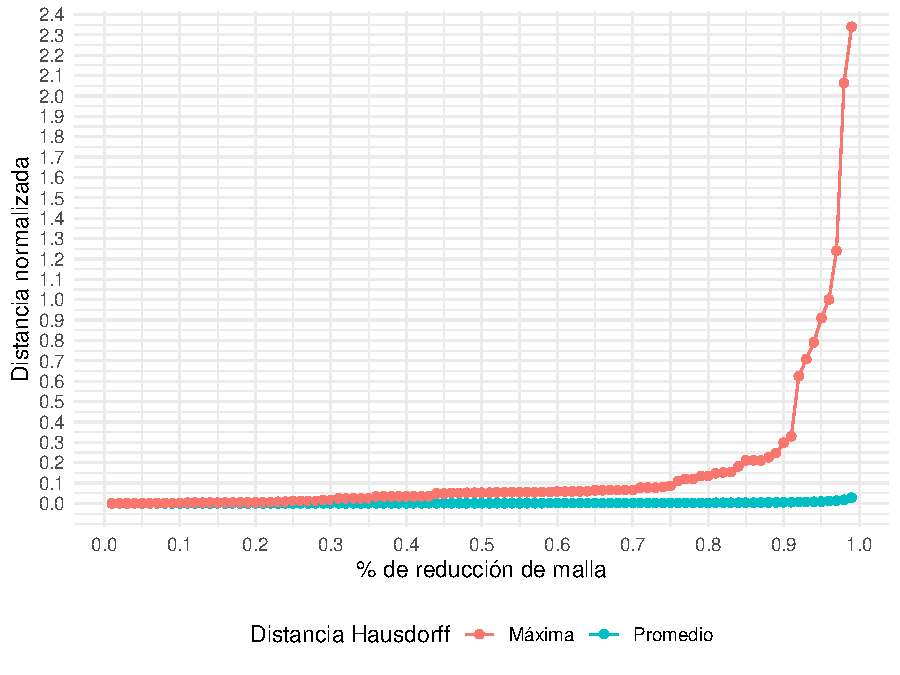
\includegraphics[width=\linewidth]{figures/5_experiments/mesh_redux_study.pdf}
    \caption[Estudio de reducción de mallas]{Distancia Hausdorff normalizada entre las mallas originales y sus versiones reducidas a distintos porcentajes del número original de triángulos. En este experimento, la reducción se realizó en incrementos del 1\%. Se observa que la distancia entre las mallas reducidas y las originales posee valores muy bajos hasta llegar al 90\% de reducción del tamaño original.}
    \label{fig5:redux_study}
\end{figure}

Para abordar esta cuestión, se diseñó un experimento en el que se toma una malla original y se generan versiones reducidas conservando distintas proporciones del número de triángulos originales (por ejemplo, 75\%, 50\%, 25\%, etc.). Posteriormente, estas versiones simplificadas se comparan con la malla original utilizando la distancia de Hausdorff, con el fin de cuantificar la desviación de la superficie resultante respecto de la original.

En la Figura \ref{fig5:redux_study} se presenta la evolución de la distancia Hausdorff normalizada al reducir progresivamente el número de triángulos de las mallas. Esta distancia ha sido normalizada respecto a la diagonal de la \textit{bounding box} de cada malla original, lo que permite comparar directamente las deformaciones relativas entre mallas de diferentes tamaños y complejidades geométricas. Además, esta normalización facilita el cálculo de promedios globales entre las distintas muestras evaluadas.

Como puede observarse, hasta una reducción del 75\% del número de triángulos, el error promedio permanece esencialmente cercano a cero, lo que sugiere una alta fidelidad en la preservación de la geometría original. Durante este mismo rango, el error máximo crece lentamente, manteniéndose al rededor del 0.2\% de variación con respecto a la malla original. Es únicamente a partir de reducciones superiores al 90\% cuando se observa un incremento más pronunciado del error máximo, aunque el error promedio aún se mantiene relativamente controlado.

Estos resultados apuntan a que es posible aplicar reducciones agresivas en la cantidad de triángulos sin comprometer significativamente la calidad topológica de las mallas. En consecuencia, se valida la viabilidad de utilizar versiones simplificadas de las mallas para el entrenamiento por medio de ExMeshCNN.

\subsection{Experimentos con etiqueta única}
Una vez validado que es factible utilizar versiones reducidas de las mallas sin pérdida significativa de información, y habiendo preparado los datos para su uso con el modelo ExMeshCNN, tal como se describe en la Sección \ref{section4:data_preparation}, se procedió a diseñar la estrategia para la generación automática de arquitecturas, explicada en profundidad en la Sección \ref{section4:nas}.

En esta fase, se llevaron a cabo los denominados experimentos de etiqueta única, donde se entrena un modelo independiente para cada una de las características de Todd, sin considerar la influencia de las demás características.

Por cada característica, se realizaron 6 ejecuciones distintas resultantes de las combinaciones de los siguientes parámetros:

\begin{itemize}
\item \textbf{Resolución de la malla}: 100,000 (o 100K); 50,000 (50K) y 25,000 (25K) triángulos.
\item \textbf{Tipo de malla}: Malla completa (Full) o malla recortada (Cut).
\end{itemize}

Cada ejecución implicó la realización de 200 entrenamientos utilizando Optuna para la búsqueda de arquitectura neuronal y optimización de hiperparámetros, con el fin de obtener el modelo más adecuado para predecir cada característica de forma individual.

Dado que se tienen 9 características de Todd, y para cada una se ejecutaron 6 combinaciones con 200 entrenamientos, el número total de entrenamientos realizados asciende a $9\times6\times200=10,800$ entrenamientos totales.

Esto equivale a $1,800$ entrenamientos por característica, lo que refleja el alto grado de exploración llevado a cabo para asegurar un modelo óptimo en cada caso.

\begin{table}[h]
    \centering
    \begin{tabular}{|c|c|c|c|c|}
    \hline
    \rowcolor[HTML]{D33333} 
    {\color[HTML]{FFFFFF} Característica} & {\color[HTML]{FFFFFF} Test Accuracy} & {\color[HTML]{FFFFFF} Test F1} & {\color[HTML]{FFFFFF} Resolución} & {\color[HTML]{FFFFFF} Tipo} \\ \hline
    AF & 0.6546 & 0.4729 & 50K & Cut \\
    BN & 0.9158 & 0.6916 & 25K & Cut \\
    DM & 0.7333 & 0.6261 & 25K & Cut \\
    DP & 0.8827 & 0.7113 & 25K & Cut \\
    IP & 0.7113 & 0.5410 & 100K & Cut \\
    LSE & 0.9800 & 0.9232 & 100K & Full \\
    USE & 0.9797 & 0.8281 & 25K & Cut \\
    VB & 0.5202 & 0.5275 & 50K & Cut \\
    VM & 0.6954 & 0.6747 & 50K & Cut \\ \hline
    \end{tabular}
    \caption{Cuadro resumen de los mejores modelos obtenidos para cada característica}
    \label{table5:single_tag__results}
\end{table}

Como se puede observar en la Tabla \ref{table5:single_tag__results}, existe una considerable variabilidad en los valores obtenidos para la métrica F1 al evaluar cada modelo sobre el conjunto de test. No obstante, en la mayoría de los casos se han alcanzado resultados satisfactorios, con valores de F1 superiores a 0.5 en todos los modelos, además de un \textit{accuracy} generalmente elevado.

Es particularmente destacable el desempeño de las características LSE y USE, que han alcanzado resultados sobresalientes a pesar de presentar un alto grado de desbalance en las etiquetas, como se evidenció en el EDA (Sección \ref{section4:data_eda}). Esto sugiere la presencia de patrones bien definidos en la superficie ósea que han sido correctamente capturados por los modelos, permitiendo lograr simultáneamente un \textit{accuracy} muy alto y valores de F1 igualmente notables. En contraste, otras dos características también altamente desbalanceadas, como BN y DP, si bien obtuvieron buenos resultados, se encuentran dentro del rango de desempeño general de las demás características más balanceadas, lo que refuerza la hipótesis de que LSE y USE presentan una topología más informativa o distinguible para las redes.

Por otro lado, la característica VB, que presenta la distribución más balanceada de etiquetas, fue la que obtuvo el rendimiento más bajo tanto en términos de \textit{accuracy} como de F1. Esto podría indicar que, pese a un buen balance, los patrones topológicos asociados a esta característica son más sutiles o complejos de identificar, lo cual plantea un reto adicional para el modelo.

El resto de las características muestran un comportamiento relativamente uniforme, sin una clara correlación entre el grado de desbalance y el rendimiento del modelo, lo que a su vez sugiere que el enfoque de entrenamiento adoptado ha sido eficaz para extraer información relevante incluso en escenarios con clases altamente desbalanceadas y una cantidad limitada de datos.

Un aspecto adicional a destacar es el impacto del tipo de malla utilizada. Exceptuando el modelo de LSE, todos los demás alcanzaron mejores resultados al emplear las versiones recortadas de las mallas. Este comportamiento respalda la hipótesis de que eliminar estructuras óseas irrelevantes (según la práctica de los expertos) permite concentrar el poder de representación del modelo en la zona de interés, reduciendo el ruido y facilitando la identificación de patrones significativos. En el caso de LSE, sin embargo, las mallas completas resultaron más beneficiosas, lo cual podría implicar que la información relevante para esta característica se encuentra distribuida también fuera de la región habitualmente considerada como de interés.

Respecto a la resolución, se observa que los mejores resultados, en general, se obtuvieron con la resolución más baja de 25K triángulos, seguida de 50K, y solo dos modelos alcanzaron su mejor desempeño con 100K triángulos. Esta observación concuerda con lo reportado por los autores de ExMeshCNN \cite{kim_exmeshcnn_2022}, donde también se encontró que las mallas de menor resolución producían mejores resultados. Se teoriza que esto se debe a que, al aumentar la resolución, la operación de \textit{global average pooling} que conecta las capas convolucionales con las totalmente conectadas podría estar diluyendo información crítica al comprimir un mayor número de triángulos en una única representación.

Sin embargo, las características LSE e IP constituyen una excepción a esta tendencia: en ambos casos, la mayor resolución permitió obtener un mejor rendimiento, lo que indica que para estas características el mayor nivel de detalle en la superficie ósea proporciona una ventaja en el aprendizaje del modelo.

\subsection{Experimentos multietiqueta}
Una vez realizados los experimentos de etiqueta única, se procedió a entrenar modelos capaces de predecir múltiples características simultáneamente. Para ello, se empleó el enfoque de \textit{multi-label classification}, que permite que cada muestra del conjunto de datos pueda estar asociada a más de una etiqueta, en contraste con la clasificación tradicional donde cada muestra pertenece a una única clase.

Para estos experimentos, primero se realizaron ejecuciones con todas las características de Todd por cada resolución, tipo de malla y, adicionalmente, dos configuraciones de la parte densa o totalmente conectada del modelo: una donde todas las salidas poseen la misma estructura y otra donde cada salida tiene una estructura densa independiente.

Posteriormente se realizaron experimentos con la mejor configuración obtenida en los resultados de etiqueta única para cada característica y las 3 características que presentan mayor correlación a la misma, como se puede observar en la Tabla \ref{table4:corr}, variando las dos configuraciones de la parte densa de la red.

Se realizaron $2 \times 2 \times 3 \times 200 = 2,400$ experimentos con todas las características, $9 \times 2 \times 200 = 3,600$ experimentos con las top 3 características con mayor asociación a una característica dada. De estos 6000 entrenamientos, en la Tabla \ref{table5:multilabel_results} se muestran los resultados de los mejores modelos obtenidos para cada característica.

\begin{table}[h]
    \centering
    \resizebox{\textwidth}{!}{%
    \begin{tabular}{|cc|c|c|c|c|c|}
        \hline
        \rowcolor[HTML]{D33333} 
        \multicolumn{2}{|c|}{\cellcolor[HTML]{D33333}{\color[HTML]{FFFFFF} \textbf{Característica}}} & \cellcolor[HTML]{D33333}{\color[HTML]{FFFFFF} } & \cellcolor[HTML]{D33333}{\color[HTML]{FFFFFF} } & \cellcolor[HTML]{D33333}{\color[HTML]{FFFFFF} } & \cellcolor[HTML]{D33333}{\color[HTML]{FFFFFF} } & \cellcolor[HTML]{D33333}{\color[HTML]{FFFFFF} } \\ \cline{1-2}
        \rowcolor[HTML]{D33333} 
        \multicolumn{1}{|c|}{\cellcolor[HTML]{D33333}{\color[HTML]{FFFFFF} \textbf{Evaluada}}} & {\color[HTML]{FFFFFF} \textbf{Soporte}} & \multirow{-2}{*}{\cellcolor[HTML]{D33333}{\color[HTML]{FFFFFF} \textbf{\begin{tabular}[c]{@{}c@{}}Test \\ Acc\end{tabular}}}} & \multirow{-2}{*}{\cellcolor[HTML]{D33333}{\color[HTML]{FFFFFF} \textbf{\begin{tabular}[c]{@{}c@{}}Test \\ F1\end{tabular}}}} & \multirow{-2}{*}{\cellcolor[HTML]{D33333}{\color[HTML]{FFFFFF} \textbf{Resolución}}} & \multirow{-2}{*}{\cellcolor[HTML]{D33333}{\color[HTML]{FFFFFF} \textbf{Hueso}}} & \multirow{-2}{*}{\cellcolor[HTML]{D33333}{\color[HTML]{FFFFFF} \textbf{Estructura Densa}}} \\ \hline
        \multicolumn{1}{|c|}{AF} & DM, LSE, USE & 0.6888 & 0.5164 & 50K & Cut & Variable \\
        \multicolumn{1}{|c|}{BN} & AF, DP, LSE & 0.9141 & 0.7869 & 25K & Cut & Variable \\
        \multicolumn{1}{|c|}{DM} & Todas & 0.7980 & 0.6525 & 100K & Cut & Same \\
        \multicolumn{1}{|c|}{DP} & Todas & 0.9261 & 0.7215 & 100K & Cut & Same \\
        \multicolumn{1}{|c|}{IP} & Todas & 0.6749 & 0.4777 & 50K & Full & Same \\
        \multicolumn{1}{|c|}{LSE} & DM, USE, VM & 0.9495 & 0.7942 & 100K & Full & Variable \\
        \multicolumn{1}{|c|}{USE} & AF, DM, LSE & 0.9541 & 0.8588 & 25K & Cut & Same \\
        \multicolumn{1}{|c|}{VB} & Todas & 0.4926 & 0.4775 & 50K & Cut & Same \\
        \multicolumn{1}{|c|}{VM} & AF, DM, IP & 0.6954 & 0.4975 & 100K & Cut & Variable \\ \hline
    \end{tabular}%
    }
    \caption{Resultados de los mejores modelos obtenidos para cada característica en los experimentos multietiqueta.}
    \label{table5:multilabel_results}
    \end{table}

De los resultados obtenidos, se observa que existe más variedad respecto a la resolución de las mallas empleadas. Soprevisamente, se encuentran casi de forma equitativa las resoluciones de 25K, 50K y 100K triángulos, con 4 modelos utilizando 100K, 3 modelos con 50K y 2 modelos con 25K. Esto contrasta con los experimentos de etiqueta única, donde la mayoría de los modelos se entrenaron con mallas de 25K triángulos. Esto resulta interesante porque sugiere que, al entrenar modelos multietiqueta, la información contenida en las mallas de mayor resolución puede ser más relevante para la predicción de múltiples características simultáneamente.

Por parte de los tipos de malla, esto se ha mantenido constante respecto a los experimentos de etiqueta única, ya que la mayoría de los modelos se entrenaron con mallas recortadas (Cut), excepto en el caso de las características LSE e IP, que emplearon mallas completas (Full). Esto refuerza la idea de que, para ciertas características, la información contenida en las zonas no recortadas es crucial para lograr un buen rendimiento del modelo incluso en un contexto multietiqueta.

En cuanto a la estructura de las capas totalmente conectadas, se observa que no hay una preferencia clara entre las distintas configuraciones, estando distribuidas casi equitativamente, esto sugiere que la elección de la estructura densa puede depender más de la naturaleza específica de las características a predecir que de una tendencia generalizada.

Sobre las características de soporte, nuevamente se encuentra una distribución casi equitativa entre hacer uso de todas las características o las tres más correlacionadas con la característica a predecir. Esto indica que, al entrenar modelos multietiqueta, es beneficioso considerar un conjunto amplio de características para mejorar la capacidad predictiva del modelo, no existiendo una tendencia clara hacia un enfoque u otro, al menos en estos experimentos.

\begin{table}[h]
    \centering
    \begin{tabular}{|c|cc|cc|}
        \hline
        \rowcolor[HTML]{D33333} 
        \cellcolor[HTML]{D33333}{\color[HTML]{FFFFFF} } & \multicolumn{2}{c|}{\cellcolor[HTML]{D33333}{\color[HTML]{FFFFFF} \textbf{Etiqueta Única}}} & \multicolumn{2}{c|}{\cellcolor[HTML]{D33333}{\color[HTML]{FFFFFF} \textbf{Etiqueta Múltiple}}} \\ \cline{2-5} 
        \rowcolor[HTML]{D33333} 
        \multirow{-2}{*}{\cellcolor[HTML]{D33333}{\color[HTML]{FFFFFF} \textbf{Característica}}} & \multicolumn{1}{c|}{\cellcolor[HTML]{D33333}{\color[HTML]{FFFFFF} \textbf{Test Acc}}} & {\color[HTML]{FFFFFF} \textbf{Test F1}} & \multicolumn{1}{c|}{\cellcolor[HTML]{D33333}{\color[HTML]{FFFFFF} \textbf{Test Acc}}} & {\color[HTML]{FFFFFF} \textbf{Test F1}} \\ \hline
        AF & \multicolumn{1}{c|}{0.6546} & 0.4729 & \multicolumn{1}{c|}{0.6888} & \textbf{0.5164} \\
        BN & \multicolumn{1}{c|}{0.9158} & 0.6916 & \multicolumn{1}{c|}{0.9141} & \textbf{0.7869} \\
        DM & \multicolumn{1}{c|}{0.7333} & 0.6261 & \multicolumn{1}{c|}{0.7980} & \textbf{0.6525} \\
        DP & \multicolumn{1}{c|}{0.8827} & 0.7113 & \multicolumn{1}{c|}{0.9261} & \textbf{0.7215} \\
        IP & \multicolumn{1}{c|}{0.7113} & \textbf{0.541} & \multicolumn{1}{c|}{0.6749} & 0.4777 \\
        LSE & \multicolumn{1}{c|}{0.9800} & \textbf{0.9232} & \multicolumn{1}{c|}{0.9495} & 0.7942 \\
        USE & \multicolumn{1}{c|}{0.9797} & 0.8281 & \multicolumn{1}{c|}{0.9541} & \textbf{0.8588} \\
        VB & \multicolumn{1}{c|}{0.5202} & \textbf{0.5275} & \multicolumn{1}{c|}{0.4926} & 0.4775 \\
        VM & \multicolumn{1}{c|}{0.6954} & \textbf{0.6747} & \multicolumn{1}{c|}{0.6954} & 0.4975 \\ \hline
    \end{tabular}
    \caption[Comparación de resultados entre los mejores modelos obtenidos en los experimentos de etiqueta única y multietiqueta]{Comparación de resultados entre los mejores modelos obtenidos en los experimentos de etiqueta única y multietiqueta. Los valores en negrita indican los mejores resultados obtenidos de la métrica F1 para cada característica.}
    \label{table5:multilabel_comparison}
\end{table}

Finalmente, se observa que los resultados obtenidos en los experimentos multietiqueta son en general superiores a los de etiqueta única, observándose la Tabla \ref{table5:multilabel_comparison}, dónde 6 de las 9 características mejoran la métrica F1 respecto a sus contrapartes de etiqueta única. Esto sugiere que el modelo es capaz de aprender patrones más complejos y representativos al considerar múltiples características simultáneamente, lo que a su vez puede mejorar la generalización del modelo y su capacidad para capturar relaciones entre las distintas características. Siendo esto consistente con la literatura consultada, donde se ha demostrado que los modelos multietiqueta pueden beneficiarse de la correlación entre las etiquetas para mejorar el rendimiento general del modelo \cite{ranjan_hyperface_2019}.

Si bien existe más disparidad respecto al \textit{accuracy} entre los experimentos de etiqueta única y multietiqueta, en general se observa que se mantiene un rendimiento alto en ambas configuraciones, con valores muy similares a los obtenidos en los experimentos de etiqueta única.

\section{Análisis de Resultados}

Durante los experimentos realizados, se ha observado que el modelo ExMeshCNN es capaz de aprender patrones topológicos relevantes en las mallas óseas para predecir las características de Todd. Los resultados obtenidos tanto en los experimentos de etiqueta única como en los de multietiqueta muestran un rendimiento prometedor, con valores de F1 y \textit{accuracy} que evidencian una buena capacidad de generalización por parte de los modelos, optimizados mediante búsqueda automática de arquitectura e hiperparámetros.

Al analizar las matrices de confusión de los mejores modelos (Figuras \ref{fig5:AF_confusion_matrix}, \ref{fig5:BN_confusion_matrix}, \ref{fig5:DM_confusion_matrix}, \ref{fig5:DP_confusion_matrix}, \ref{fig5:IP_confusion_matrix}, \ref{fig5:LSE_confusion_matrix}, \ref{fig5:USE_confusion_matrix}, \ref{fig5:VB_confusion_matrix} y \ref{fig5:VM_confusion_matrix}), se aprecia que los modelos tienden a clasificar correctamente la mayoría de las muestras de una forma equilibrada tal y como se observó con la métrica F1, cometiendo más errores en aquellas clases menos representadas. Este comportamiento es coherente con lo esperado en problemas de clasificación desbalanceada, donde los modelos suelen favorecer las clases mayoritarias. No obstante, la mayoría de las confusiones ocurren entre clases adyacentes, lo que sugiere que el modelo ha aprendido a distinguir de manera significativa los patrones de las distintas características de Todd. De forma particular, la característica con peor rendimiento es VB, que presenta una matriz de confusión con un alto número de falsos negativos, lo que indica que el modelo tiene dificultades para identificar correctamente las muestras de esta clase, a pesar de que es la característica más balanceada en términos de distribución de etiquetas. Esto concuerda con las observaciones realizadas en en ???, dónde se observó que esta característica es la que presenta la mayor tasa de error inter e intra-experto, lo que sugiere que esta es una característica más subjetiva o menos consistente entre los expertos, lo que dificulta su clasificación por parte del modelo.

\subsection{Hiperparámetros y Arquitectura Neuronal}
Para facilitar la comprensión, se incluye una tabla resumen que detalla los datos de entrada utilizados por cada modelo, así como su arquitectura y los hiperparámetros seleccionados. La Tabla \ref{table5:sample_table} muestra un ejemplo del formato empleado, junto con la explicación de cada una de sus columnas y filas.

Los mejores modelos obtenidos presentan configuraciones arquitectónicas notablemente diversas entre sí, lo que indica que la búsqueda automática ha sido efectiva para adaptar la estructura de las redes a los requerimientos específicos de cada característica.

Pese a esta diversidad, se observa una tendencia general hacia redes con mayor profundidad en las capas convolucionales, como en los casos de AF (Tabla \ref{table5:AF_best_model}), BN (Tabla \ref{table5:BN_best_model}), IP (Tabla \ref{table5:IP_best_model}), LSE (Tabla \ref{table5:LSE_best_model}), VB (Tabla \ref{table5:VB_best_model}) y VM (Tabla \ref{table5:VM_best_model}), donde se utilizaron 4 o más capas convolucionales, y algunas, como AF, BN y VM, alcanzaron hasta 6 capas. Esto sugiere que estas características pueden requerir una mayor capacidad de representación para capturar los patrones complejos presentes en las mallas.

En cuanto al número de filtros por capa, se aprecia un patrón común de expansión y contracción a lo largo de la red, posiblemente reflejando una estructura tipo cuello de botella. USE (Tabla \ref{table5:USE_best_model}) es la única excepción donde este patrón no se manifiesta claramente.

Las capas totalmente conectadas, en cambio, presentan mayor variabilidad en cuanto al número de neuronas y estructura, sin un patrón claro, lo que indica una fuerte dependencia del diseño respecto a la tarea específica.

En términos de hiperparámetros, se detecta un uso consistente del optimizador Adam y de la inicialización Kaiming en la mayoría de los modelos exitosos, lo que sugiere que estas configuraciones son adecuadas para el entrenamiento de redes basadas en ExMeshCNN. En cuanto a las funciones de pérdida, predomina el uso de WCE, seguida por CBL, lo cual es coherente con la naturaleza desbalanceada del problema y valida su idoneidad para este tipo de clasificación.

\begin{figure}[p]
    \begin{minipage}{\linewidth}
        \centering
        \begin{tabular}{c|cc|c|c|}
            \hline
            \rowcolor[HTML]{D33333} 
            \multicolumn{1}{|c|}{\cellcolor[HTML]{D33333}{\color[HTML]{FFFFFF} }} & \multicolumn{2}{c|}{\cellcolor[HTML]{D33333}{\color[HTML]{FFFFFF} \textbf{DECR}}} & {\color[HTML]{FFFFFF} \textbf{CONV}} & {\color[HTML]{FFFFFF} \textbf{FN}} \\ \cline{2-5} 
            \multicolumn{1}{|c|}{\multirow{-2}{*}{\cellcolor[HTML]{D33333}{\color[HTML]{FFFFFF} \textbf{DATA}}}} & \multicolumn{2}{c|}{\cellcolor[HTML]{D33333}{\color[HTML]{FFFFFF} \textbf{GEOD}}} &  & \textbf{(h)} \\ \cline{1-3} \cline{5-5} 
            \multicolumn{1}{|c|}{\cellcolor[HTML]{D33333}{\color[HTML]{FFFFFF} \textbf{RES}}} & MID & (c) &  &  \\ \cline{1-1}
            \multicolumn{1}{|c|}{(a)} & OUT & (d) &  &  \\ \cline{1-3}
            \multicolumn{1}{|c|}{\cellcolor[HTML]{D33333}{\color[HTML]{FFFFFF} \textbf{TYPE}}} & \multicolumn{2}{c|}{\cellcolor[HTML]{D33333}{\color[HTML]{FFFFFF} \textbf{GEOM}}} &  &  \\ \cline{1-3}
            \multicolumn{1}{|c|}{(b)} & MID & (e) &  &  \\ \cline{1-1}
             & OUT & (f) & \multirow{-6}{*}{(g)} & \multirow{-5}{*}{(i)} \\ \cline{2-5} 
        \end{tabular}
    
        \vspace{1em}
    
        \begin{tabular}{|
            >{\columncolor[HTML]{D33333}}c |c|c|}
            \hline
            {\color[HTML]{FFFFFF} \textbf{LR}} & (j) & \cellcolor[HTML]{D33333}{\color[HTML]{FFFFFF} \textbf{LOSS}} \\ \hline
            {\color[HTML]{FFFFFF} \textbf{OPTIMIZER}} & (k) & \textbf{(h)} \\ \hline
            {\color[HTML]{FFFFFF} \textbf{INIT}} & (l) & (n) \\ \hline
        \end{tabular}
        \captionof{table}[Formato de tabla usado para resumir los datos de entrada, la estructura de la red y los hiperparámetros de los mejores modelos]{Formato utilizado para resumir los datos de entrada, la estructura de la red y los hiperparámetros empleados en cada uno de los modelos. La tabla superior detalla las configuraciones relativas a los datos y la arquitectura, mientras que la tabla inferior resume los hiperparámetros principales. En la tabla superior, la columna \textbf{DATA} especifica las características de los datos de entrada: \textbf{RES} indica la resolución de la malla (a) y \textbf{TYPE} su tipo (b). La columna \textbf{DECR} incluye la configuración de los descriptores utilizados: \textbf{GEOD} para el descriptor geodésico y \textbf{GEOM} para el descriptor geométrico; MID y OUT indican respectivamente la densidad de sus capas intermedias (c, e) y de salida (d, f). La columna \textbf{CONV} muestra la arquitectura de las capas convolucionales: número de capas y densidad de cada una (g). La columna \textbf{FN} presenta en (h) las características morfológicas predichas y en (i) la configuración de la parte densa del modelo de cada una. En la tabla inferior, \textbf{LR} indica la tasa de aprendizaje (j), \textbf{OPTIMIZER} el optimizador empleado (k), \textbf{INIT} el tipo de inicialización de pesos (l), y \textbf{LOSS} la función de pérdida (n) asociada a la característica correspondiente (h).}
        \label{table5:sample_table}
    \end{minipage}
\end{figure}

%% AF
\begin{figure}[htbp]
    \centering
    % --- Top: Table ---
    \begin{minipage}{\linewidth}
        \centering
        \begin{tabular}{c|cc|c|cccc|}
            \hline
            \rowcolor[HTML]{D33333} 
            \multicolumn{1}{|c|}{\cellcolor[HTML]{D33333}{\color[HTML]{FFFFFF} }} & \multicolumn{2}{c|}{\cellcolor[HTML]{D33333}{\color[HTML]{FFFFFF} \textbf{DECR}}} & {\color[HTML]{FFFFFF} \textbf{CONV}} & \multicolumn{4}{c|}{\cellcolor[HTML]{D33333}{\color[HTML]{FFFFFF} \textbf{FN}}} \\ \cline{2-8} 
            \multicolumn{1}{|c|}{\multirow{-2}{*}{\cellcolor[HTML]{D33333}{\color[HTML]{FFFFFF} \textbf{DATA}}}} & \multicolumn{2}{c|}{\cellcolor[HTML]{D33333}{\color[HTML]{FFFFFF} \textbf{GEOD}}} & 64 & \multicolumn{1}{c|}{\cellcolor[HTML]{FFCCC9}\textbf{AF}} & \multicolumn{1}{c|}{\cellcolor[HTML]{FFFFFF}\textbf{DM}} & \multicolumn{1}{c|}{\textbf{LSE}} & \textbf{USE} \\ \cline{1-3} \cline{5-8} 
            \multicolumn{1}{|c|}{\cellcolor[HTML]{D33333}{\color[HTML]{FFFFFF} \textbf{RES}}} & MID & 16 & 32 & \multicolumn{1}{c|}{\cellcolor[HTML]{FFCCC9}256} & \multicolumn{1}{c|}{\cellcolor[HTML]{FFFFFF}8} & \multicolumn{1}{c|}{16} & 32 \\ \cline{1-1} \cline{5-6}
            \multicolumn{1}{|c|}{50K} & OUT & 128 & 32 &  & \multicolumn{1}{c|}{\cellcolor[HTML]{FFFFFF}} & \multicolumn{1}{c|}{8} & 32 \\ \cline{1-3}
            \multicolumn{1}{|c|}{\cellcolor[HTML]{D33333}{\color[HTML]{FFFFFF} \textbf{TYPE}}} & \multicolumn{2}{c|}{\cellcolor[HTML]{D33333}{\color[HTML]{FFFFFF} \textbf{GEOM}}} & 128 &  & \multicolumn{1}{c|}{} & \multicolumn{1}{c|}{64} & 256 \\ \cline{1-3}
            \multicolumn{1}{|c|}{Cut} & MID & 128 & 256 &  & \multicolumn{1}{c|}{} & \multicolumn{1}{c|}{128} & 64 \\ \cline{1-1} \cline{7-7}
             & OUT & 256 & 32 &  &  & \multicolumn{1}{c|}{} & 16 \\ \cline{2-4} \cline{8-8} 
        \end{tabular}

        \vspace{1em}

        \begin{tabular}{|
            >{\columncolor[HTML]{D33333}}c |c|
            >{\columncolor[HTML]{FFCCC9}}c ccc|}
            \hline
            {\color[HTML]{FFFFFF} \textbf{LR}} & $3.4261 \times 10^{-4}$ & \multicolumn{4}{c|}{\cellcolor[HTML]{D33333}{\color[HTML]{FFFFFF} \textbf{LOSS}}} \\ \hline
            {\color[HTML]{FFFFFF} \textbf{OPTIMIZER}} & AdamW & \multicolumn{1}{c|}{\cellcolor[HTML]{FFCCC9}\textbf{AF}} & \multicolumn{1}{c|}{\textbf{DM}} & \multicolumn{1}{c|}{\textbf{LSE}} & \textbf{USE} \\ \hline
            {\color[HTML]{FFFFFF} \textbf{INIT}} & N/A & \multicolumn{1}{c|}{\cellcolor[HTML]{FFCCC9}WCE} & \multicolumn{1}{c|}{WCE} & \multicolumn{1}{c|}{CE} & WCE \\ \hline
        \end{tabular}
        \captionof{table}{Característica AF: Datos de entrada, estructura de red e hiperparámetros del mejor modelo.}
        \label{table5:AF_best_model}
    \end{minipage}

    \vspace{1.5em} % vertical space between table and image

    % --- Bottom: Figure ---
    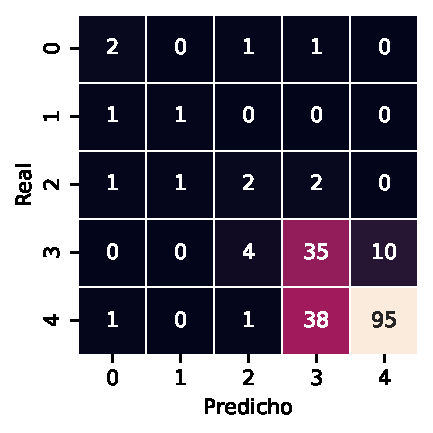
\includegraphics[width=0.6\linewidth]{figures/5_experiments/multi-af-cm.pdf}
    \caption[Característica AF: Matriz de confusión del mejor modelo en datos de test]{Característica \textbf{AF}: Matriz de confusión del mejor modelo en datos de test. Leyenda: \textbf{0}: Porosidad Regular, \textbf{1}: Muy Definidas, \textbf{2}: Poco Profundas, \textbf{3}: Restos de Surcos, \textbf{4}: No hay surcos.}
    \label{fig5:AF_confusion_matrix}
\end{figure}

%% BN
\begin{figure}[htbp]
    \centering
    % --- Top: Table ---
    \begin{minipage}{\linewidth}
        \centering
        \begin{tabular}{c|cc|c|cccc}
            \hline
            \rowcolor[HTML]{D33333} 
            \multicolumn{1}{|c|}{\cellcolor[HTML]{D33333}{\color[HTML]{FFFFFF} }} & \multicolumn{2}{c|}{\cellcolor[HTML]{D33333}{\color[HTML]{FFFFFF} \textbf{DECR}}} & {\color[HTML]{FFFFFF} \textbf{CONV}} & \multicolumn{4}{c|}{\cellcolor[HTML]{D33333}{\color[HTML]{FFFFFF} \textbf{FN}}} \\ \cline{2-8} 
            \multicolumn{1}{|c|}{\multirow{-2}{*}{\cellcolor[HTML]{D33333}{\color[HTML]{FFFFFF} \textbf{DATA}}}} & \multicolumn{2}{c|}{\cellcolor[HTML]{D33333}{\color[HTML]{FFFFFF} \textbf{GEOD}}} & 256 & \multicolumn{1}{c|}{\cellcolor[HTML]{FFFFFF}\textbf{AF}} & \multicolumn{1}{c|}{\cellcolor[HTML]{FFCCC9}\textbf{BN}} & \multicolumn{1}{c|}{\textbf{DP}} & \multicolumn{1}{c|}{\textbf{LSE}} \\ \cline{1-3} \cline{5-8} 
            \multicolumn{1}{|c|}{\cellcolor[HTML]{D33333}{\color[HTML]{FFFFFF} \textbf{RES}}} & MID & 256 & 128 & \multicolumn{1}{c|}{\cellcolor[HTML]{FFFFFF}128} & \multicolumn{1}{c|}{\cellcolor[HTML]{FFCCC9}32} & \multicolumn{1}{c|}{32} & \multicolumn{1}{c|}{32} \\ \cline{1-1} \cline{5-5}
            \multicolumn{1}{|c|}{25K} & OUT & 16 & 256 & \multicolumn{1}{c|}{} & \multicolumn{1}{c|}{\cellcolor[HTML]{FFCCC9}64} & \multicolumn{1}{c|}{64} & \multicolumn{1}{c|}{128} \\ \cline{1-3} \cline{6-6}
            \multicolumn{1}{|c|}{\cellcolor[HTML]{D33333}{\color[HTML]{FFFFFF} \textbf{TYPE}}} & \multicolumn{2}{c|}{\cellcolor[HTML]{D33333}{\color[HTML]{FFFFFF} \textbf{GEOM}}} & 64 &  & \multicolumn{1}{c|}{} & \multicolumn{1}{c|}{256} & \multicolumn{1}{c|}{128} \\ \cline{1-3} \cline{8-8} 
            \multicolumn{1}{|c|}{Cut} & MID & 32 & 16 &  & \multicolumn{1}{c|}{} & \multicolumn{1}{c|}{16} &  \\ \cline{1-1}
             & OUT & 16 & 64 &  & \multicolumn{1}{c|}{} & \multicolumn{1}{c|}{256} &  \\ \cline{2-4} \cline{7-7}
        \end{tabular}

        \vspace{1em}

        \begin{tabular}{|
            >{\columncolor[HTML]{D33333}}c |c|c
            >{\columncolor[HTML]{FFCCC9}}c cc|}
            \hline
            {\color[HTML]{FFFFFF} \textbf{LR}} & $5.0965 \times 10^{-3}$ & \multicolumn{4}{c|}{\cellcolor[HTML]{D33333}{\color[HTML]{FFFFFF} \textbf{LOSS}}} \\ \hline
            {\color[HTML]{FFFFFF} \textbf{OPTIMIZER}} & Radam & \multicolumn{1}{c|}{\textbf{AF}} & \multicolumn{1}{c|}{\cellcolor[HTML]{FFCCC9}\textbf{BN}} & \multicolumn{1}{c|}{\textbf{DP}} & \textbf{LSE} \\ \hline
            {\color[HTML]{FFFFFF} \textbf{INIT}} & Kaiming & \multicolumn{1}{c|}{FL} & \multicolumn{1}{c|}{\cellcolor[HTML]{FFCCC9}CBL} & \multicolumn{1}{c|}{CBL} & CBL \\ \hline
        \end{tabular}
        \captionof{table}{Característica BN: Datos de entrada, estructura de red e hiperparámetros del mejor modelo.}
        \label{table5:BN_best_model}
    \end{minipage}

    \vspace{1.5em} % vertical space between table and image

    % --- Bottom: Figure ---
    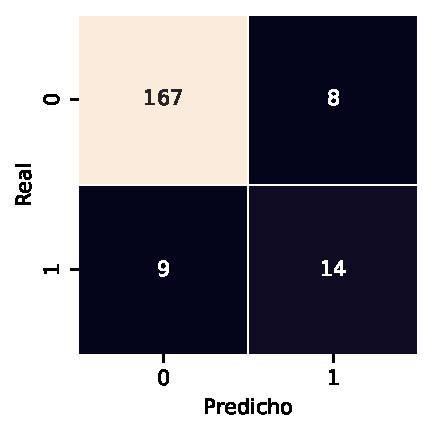
\includegraphics[width=0.6\linewidth]{figures/5_experiments/multi-bn-cm.pdf}
    \caption[Característica BN: Matriz de confusión del mejor modelo en datos de test.]{Característica BN: Matriz de confusión del mejor modelo en datos de test. Leyenda: \textbf{0}: Ausente, \textbf{1}: Presente.}
    \label{fig5:BN_confusion_matrix}
\end{figure}

%% DM / DP
\begin{figure}[htbp]
    \centering
    % --- Top: Table ---
    \begin{minipage}{\linewidth}
        \centering
        \begin{tabular}{c|cc|cc}
            \hline
            \rowcolor[HTML]{D33333} 
            \multicolumn{1}{|c|}{\cellcolor[HTML]{D33333}{\color[HTML]{FFFFFF} }} & \multicolumn{2}{c|}{\cellcolor[HTML]{D33333}{\color[HTML]{FFFFFF} \textbf{DECR}}} & \multicolumn{1}{c|}{\cellcolor[HTML]{D33333}{\color[HTML]{FFFFFF} \textbf{CONV}}} & \multicolumn{1}{c|}{\cellcolor[HTML]{D33333}{\color[HTML]{FFFFFF} \textbf{FN}}} \\ \cline{2-5} 
            \multicolumn{1}{|c|}{\multirow{-2}{*}{\cellcolor[HTML]{D33333}{\color[HTML]{FFFFFF} \textbf{DATA}}}} & \multicolumn{2}{c|}{\cellcolor[HTML]{D33333}{\color[HTML]{FFFFFF} \textbf{GEOD}}} & \multicolumn{1}{c|}{64} & \multicolumn{1}{c|}{\textbf{Todos}} \\ \cline{1-3} \cline{5-5} 
            \multicolumn{1}{|c|}{\cellcolor[HTML]{D33333}{\color[HTML]{FFFFFF} \textbf{RES}}} & MID & 16 & \multicolumn{1}{c|}{128} & \multicolumn{1}{c|}{32} \\ \cline{1-1} \cline{5-5} 
            \multicolumn{1}{|c|}{100K} & OUT & 16 & \multicolumn{1}{c|}{128} &  \\ \cline{1-4}
            \multicolumn{1}{|c|}{\cellcolor[HTML]{D33333}{\color[HTML]{FFFFFF} \textbf{TYPE}}} & \multicolumn{2}{c|}{\cellcolor[HTML]{D33333}{\color[HTML]{FFFFFF} \textbf{GEOM}}} &  &  \\ \cline{1-3}
            \multicolumn{1}{|c|}{Cut} & MID & 16 &  &  \\ \cline{1-1}
             & OUT & 256 &  &  \\ \cline{2-3}
        \end{tabular}

        \vspace{1em}

        \begin{tabular}{cc|ccccc}
        \hline
        \multicolumn{1}{|c|}{\cellcolor[HTML]{D33333}{\color[HTML]{FFFFFF} \textbf{LR}}} & $1.4861 \times 10^{-4}$ & \multicolumn{5}{c|}{\cellcolor[HTML]{D33333}{\color[HTML]{FFFFFF} \textbf{LOSS}}} \\ \hline
        \multicolumn{1}{|c|}{\cellcolor[HTML]{D33333}{\color[HTML]{FFFFFF} \textbf{OPTIMIZER}}} & Adam & \multicolumn{1}{c|}{\textbf{AF}} & \multicolumn{1}{c|}{\textbf{BN}} & \multicolumn{1}{c|}{\cellcolor[HTML]{FFCCC9}\textbf{DM}} & \multicolumn{1}{c|}{\cellcolor[HTML]{FFCCC9}\textbf{DP}} & \multicolumn{1}{c|}{\textbf{IP}} \\ \hline
        \multicolumn{1}{|c|}{\cellcolor[HTML]{D33333}{\color[HTML]{FFFFFF} \textbf{INIT}}} & Kaiming & \multicolumn{1}{c|}{WCE} & \multicolumn{1}{c|}{CE} & \multicolumn{1}{c|}{\cellcolor[HTML]{FFCCC9}CE} & \multicolumn{1}{c|}{\cellcolor[HTML]{FFCCC9}CE} & \multicolumn{1}{c|}{WCE} \\ \hline
        &  & \multicolumn{1}{c|}{\textbf{LSE}} & \multicolumn{1}{c|}{\textbf{USE}} & \multicolumn{1}{c|}{\textbf{VB}} & \multicolumn{1}{c|}{\textbf{VM}} &  \\ \cline{3-6}
        &  & \multicolumn{1}{c|}{CE} & \multicolumn{1}{c|}{WCE} & \multicolumn{1}{c|}{CE} & \multicolumn{1}{c|}{CE} &  \\ \cline{3-6}
        \end{tabular}
        \captionof{table}{Características DP y DM: Datos de entrada, estructura de red e hiperparámetros del mejor modelo.}
        \label{table5:DM_DP_best_model}
    \end{minipage}

    \vspace{1.5em} % vertical space between table and image

    % --- Bottom: Figure ---
    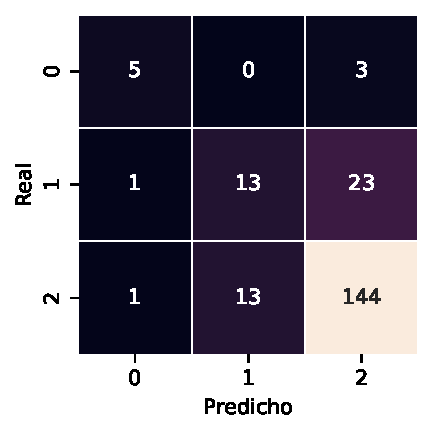
\includegraphics[width=0.4\linewidth]{figures/5_experiments/multi-dm-cm.pdf}
    \caption[Característica DM: Matriz de confusión del mejor modelo en datos de test.]{Característica \textbf{DM}: Matriz de confusión del mejor modelo en datos de test. Leyenda: \textbf{0}: No Definido, \textbf{1}: En Formación, \textbf{2}: Definido.}
    \label{fig5:DM_confusion_matrix}
    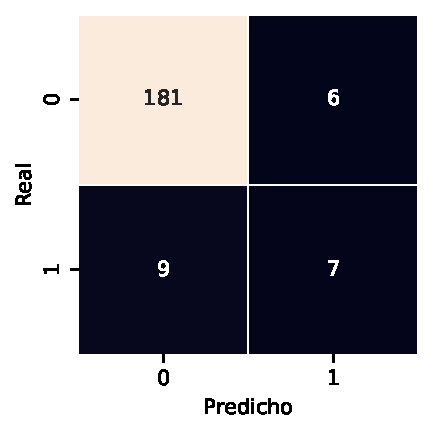
\includegraphics[width=0.4\linewidth]{figures/5_experiments/multi-dp-cm.pdf}
    \caption[Característica DP: Matriz de confusión del mejor modelo en datos de test.]{Característica DP: Matriz de confusión del mejor modelo en datos de test. Leyenda: \textbf{0}: Ausente, \textbf{1}: Presente.}
    \label{fig5:DP_confusion_matrix}
\end{figure}

%% IP
\begin{figure}[htbp]
    \centering
    % --- Top: Table ---
    \begin{minipage}{\linewidth}
        \centering
        \begin{tabular}{c|cc|cc}
            \hline
            \rowcolor[HTML]{D33333} 
            \multicolumn{1}{|c|}{\cellcolor[HTML]{D33333}{\color[HTML]{FFFFFF} }} & \multicolumn{2}{c|}{\cellcolor[HTML]{D33333}{\color[HTML]{FFFFFF} \textbf{DECR}}} & \multicolumn{1}{c|}{\cellcolor[HTML]{D33333}{\color[HTML]{FFFFFF} \textbf{CONV}}} & \multicolumn{1}{c|}{\cellcolor[HTML]{D33333}{\color[HTML]{FFFFFF} \textbf{FN}}} \\ \cline{2-5} 
            \multicolumn{1}{|c|}{\multirow{-2}{*}{\cellcolor[HTML]{D33333}{\color[HTML]{FFFFFF} \textbf{DATA}}}} & \multicolumn{2}{c|}{\cellcolor[HTML]{D33333}{\color[HTML]{FFFFFF} \textbf{GEOD}}} & \multicolumn{1}{c|}{64} & \multicolumn{1}{c|}{\textbf{IP}} \\ \cline{1-3} \cline{5-5} 
            \multicolumn{1}{|c|}{\cellcolor[HTML]{D33333}{\color[HTML]{FFFFFF} \textbf{RES}}} & MID & 256 & \multicolumn{1}{c|}{128} & \multicolumn{1}{c|}{256} \\ \cline{1-1} \cline{5-5} 
            \multicolumn{1}{|c|}{100K} & OUT & 32 & \multicolumn{1}{c|}{64} &  \\ \cline{1-3}
            \multicolumn{1}{|c|}{\cellcolor[HTML]{D33333}{\color[HTML]{FFFFFF} \textbf{TYPE}}} & \multicolumn{2}{c|}{\cellcolor[HTML]{D33333}{\color[HTML]{FFFFFF} \textbf{GEOM}}} & \multicolumn{1}{c|}{64} &  \\ \cline{1-3}
            \multicolumn{1}{|c|}{Cut} & MID & 16 & \multicolumn{1}{c|}{32} &  \\ \cline{1-1} \cline{4-4}
             & OUT & 256 &  &  \\ \cline{2-3}
        \end{tabular}

        \vspace{1em}

        \begin{tabular}{|
            >{\columncolor[HTML]{D33333}}c |c|c|}
            \hline
            {\color[HTML]{FFFFFF} \textbf{LR}} & $1.2990 \times 10^{-3}$ & \cellcolor[HTML]{D33333}{\color[HTML]{FFFFFF} \textbf{LOSS}} \\ \hline
            {\color[HTML]{FFFFFF} \textbf{OPTIMIZER}} & Radam & \textbf{IP} \\ \hline
            {\color[HTML]{FFFFFF} \textbf{INIT}} & Kaiming & WCE \\ \hline
        \end{tabular}
        \captionof{table}{Característica IP: Datos de entrada, estructura de red e hiperparámetros del mejor modelo.}
        \label{table5:IP_best_model}
    \end{minipage}

    \vspace{1.5em} % vertical space between table and image

    % --- Bottom: Figure ---
    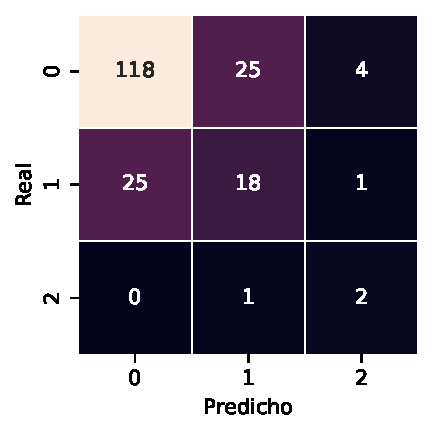
\includegraphics[width=0.6\linewidth]{figures/5_experiments/single-ip-cm.pdf}
    \caption[Característica IP: Matriz de confusión del mejor modelo en datos de test.]{Característica IP: Matriz de confusión del mejor modelo en datos de test. Leyenda: \textbf{0}: No, \textbf{1}: Mediana, \textbf{2}: Sí.}
    \label{fig5:IP_confusion_matrix}
\end{figure}

%% LSE
\begin{figure}[htbp]
    \centering
    % --- Top: Table ---
    \begin{minipage}{\linewidth}
        \centering
        \begin{tabular}{c|cc|cc}
            \hline
            \rowcolor[HTML]{D33333} 
            \multicolumn{1}{|c|}{\cellcolor[HTML]{D33333}{\color[HTML]{FFFFFF} }} & \multicolumn{2}{c|}{\cellcolor[HTML]{D33333}{\color[HTML]{FFFFFF} \textbf{DECR}}} & \multicolumn{1}{c|}{\cellcolor[HTML]{D33333}{\color[HTML]{FFFFFF} \textbf{CONV}}} & \multicolumn{1}{c|}{\cellcolor[HTML]{D33333}{\color[HTML]{FFFFFF} \textbf{FN}}} \\ \cline{2-5} 
            \multicolumn{1}{|c|}{\multirow{-2}{*}{\cellcolor[HTML]{D33333}{\color[HTML]{FFFFFF} \textbf{DATA}}}} & \multicolumn{2}{c|}{\cellcolor[HTML]{D33333}{\color[HTML]{FFFFFF} \textbf{GEOD}}} & \multicolumn{1}{c|}{256} & \multicolumn{1}{c|}{\textbf{LSE}} \\ \cline{1-3} \cline{5-5} 
            \multicolumn{1}{|c|}{\cellcolor[HTML]{D33333}{\color[HTML]{FFFFFF} \textbf{RES}}} & MID & 32 & \multicolumn{1}{c|}{16} & \multicolumn{1}{c|}{8} \\ \cline{1-1}
            \multicolumn{1}{|c|}{100K} & OUT & 64 & \multicolumn{1}{c|}{64} & \multicolumn{1}{c|}{16} \\ \cline{1-3}
            \multicolumn{1}{|c|}{\cellcolor[HTML]{D33333}{\color[HTML]{FFFFFF} \textbf{TYPE}}} & \multicolumn{2}{c|}{\cellcolor[HTML]{D33333}{\color[HTML]{FFFFFF} \textbf{GEOM}}} & \multicolumn{1}{c|}{16} & \multicolumn{1}{c|}{256} \\ \cline{1-4}
            \multicolumn{1}{|c|}{Full} & MID & 256 & \multicolumn{1}{c|}{} & \multicolumn{1}{c|}{128} \\ \cline{1-1} \cline{5-5} 
             & OUT & 128 &  &  \\ \cline{2-3}
    \end{tabular}

        \vspace{1em}

        \begin{tabular}{|
            >{\columncolor[HTML]{D33333}}l |l|l|}
            \hline
            {\color[HTML]{FFFFFF} \textbf{LR}} & $8.4586 \times 10^{-5}$ & \cellcolor[HTML]{D33333}{\color[HTML]{FFFFFF} \textbf{LOSS}} \\ \hline
            {\color[HTML]{FFFFFF} \textbf{OPTIMIZER}} & Adam & \textbf{LSE} \\ \hline
            {\color[HTML]{FFFFFF} \textbf{INIT}} & Orthogonal & WCE \\ \hline
        \end{tabular}
        \captionof{table}{Característica LSE: Datos de entrada, estructura de red e hiperparámetros del mejor modelo.}
        \label{table5:LSE_best_model}
    \end{minipage}

    \vspace{1.5em} % vertical space between table and image

    % --- Bottom: Figure ---
    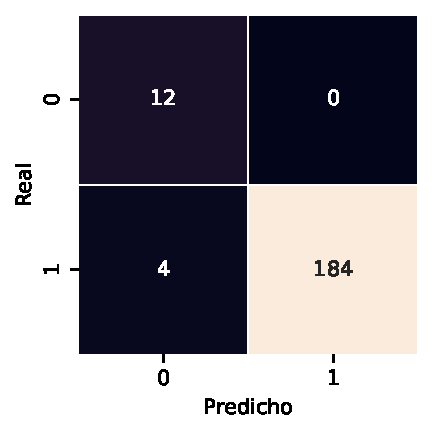
\includegraphics[width=0.6\linewidth]{figures/5_experiments/single-lse-cm.pdf}
    \caption[Característica LSE: Matriz de confusión del mejor modelo en datos de test.]{Característica LSE: Matriz de confusión del mejor modelo en datos de test. Leyenda: \textbf{0}: No Definido, \textbf{1}: Definido.}
    \label{fig5:LSE_confusion_matrix}
\end{figure}

%% USE
\begin{figure}[htbp]
    \centering
    % --- Top: Table ---
    \begin{minipage}{\linewidth}
        \centering
        \begin{tabular}{c|cc|cc}
            \hline
            \rowcolor[HTML]{D33333} 
            \multicolumn{1}{|c|}{\cellcolor[HTML]{D33333}{\color[HTML]{FFFFFF} }} & \multicolumn{2}{c|}{\cellcolor[HTML]{D33333}{\color[HTML]{FFFFFF} \textbf{DECR}}} & \multicolumn{1}{c|}{\cellcolor[HTML]{D33333}{\color[HTML]{FFFFFF} \textbf{CONV}}} & \multicolumn{1}{c|}{\cellcolor[HTML]{D33333}{\color[HTML]{FFFFFF} \textbf{FN}}} \\ \cline{2-5} 
            \multicolumn{1}{|c|}{\multirow{-2}{*}{\cellcolor[HTML]{D33333}{\color[HTML]{FFFFFF} \textbf{DATA}}}} & \multicolumn{2}{c|}{\cellcolor[HTML]{D33333}{\color[HTML]{FFFFFF} \textbf{GEOD}}} & \multicolumn{1}{c|}{32} & \multicolumn{1}{c|}{\textbf{Todos}} \\ \cline{1-3} \cline{5-5} 
            \multicolumn{1}{|c|}{\cellcolor[HTML]{D33333}{\color[HTML]{FFFFFF} \textbf{RES}}} & MID & 128 & \multicolumn{1}{c|}{32} & \multicolumn{1}{c|}{16} \\ \cline{1-1} \cline{4-5} 
            \multicolumn{1}{|c|}{25K} & OUT & 256 &  &  \\ \cline{1-3}
            \multicolumn{1}{|c|}{\cellcolor[HTML]{D33333}{\color[HTML]{FFFFFF} \textbf{TYPE}}} & \multicolumn{2}{c|}{\cellcolor[HTML]{D33333}{\color[HTML]{FFFFFF} \textbf{GEOM}}} &  &  \\ \cline{1-3}
            \multicolumn{1}{|c|}{Cut} & MID & 16 &  &  \\ \cline{1-1}
             & OUT & 32 &  &  \\ \cline{2-3}
        \end{tabular}

        \vspace{1em}

        \begin{tabular}{|
            >{\columncolor[HTML]{D33333}}c |c|ccc
            >{\columncolor[HTML]{FFCCC9}}c c|}
            \hline
            {\color[HTML]{FFFFFF} \textbf{LR}} & $1.3456 \times 10^{-3}$ & \multicolumn{5}{c|}{\cellcolor[HTML]{D33333}{\color[HTML]{FFFFFF} \textbf{LOSS}}} \\ \hline
            {\color[HTML]{FFFFFF} \textbf{OPTIMIZER}} & Adam & \multicolumn{1}{c|}{\textbf{AF}} & \multicolumn{1}{c|}{\textbf{DM}} & \multicolumn{1}{c|}{\textbf{LSE}} & \multicolumn{1}{c|}{\cellcolor[HTML]{FFCCC9}\textbf{USE}} & \textbf{IP} \\ \hline
            {\color[HTML]{FFFFFF} \textbf{INIT}} & Kaiming & \multicolumn{1}{c|}{CBL} & \multicolumn{1}{c|}{CE} & \multicolumn{1}{c|}{CBL} & \multicolumn{1}{c|}{\cellcolor[HTML]{FFCCC9}FL} & WCE \\ \hline
        \end{tabular}
        \captionof{table}{Característica USE: Datos de entrada, estructura de red e hiperparámetros del mejor modelo.}
        \label{table5:USE_best_model}
    \end{minipage}

    \vspace{1.5em} % vertical space between table and image

    % --- Bottom: Figure ---
    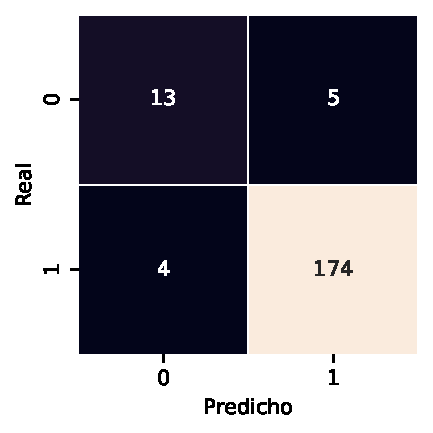
\includegraphics[width=0.6\linewidth]{figures/5_experiments/multi-use-cm.pdf}
    \caption[Característica USE: Matriz de confusión del mejor modelo en datos de test.]{Característica USE: Matriz de confusión del mejor modelo en datos de test. Leyenda: \textbf{0}: No Definido, \textbf{1}: Definido.}
    \label{fig5:USE_confusion_matrix}
\end{figure}

%% VB
\begin{figure}[htbp]
    \centering
    % --- Top: Table ---
    \begin{minipage}{\linewidth}
        \centering
        \begin{tabular}{c|cc|c|c|}
            \hline
            \rowcolor[HTML]{D33333} 
            \multicolumn{1}{|c|}{\cellcolor[HTML]{D33333}{\color[HTML]{FFFFFF} }} & \multicolumn{2}{c|}{\cellcolor[HTML]{D33333}{\color[HTML]{FFFFFF} \textbf{DECR}}} & {\color[HTML]{FFFFFF} \textbf{CONV}} & {\color[HTML]{FFFFFF} \textbf{FN}} \\ \cline{2-5} 
            \multicolumn{1}{|c|}{\multirow{-2}{*}{\cellcolor[HTML]{D33333}{\color[HTML]{FFFFFF} \textbf{DATA}}}} & \multicolumn{2}{c|}{\cellcolor[HTML]{D33333}{\color[HTML]{FFFFFF} \textbf{GEOD}}} & 64 & \textbf{VB} \\ \cline{1-3} \cline{5-5} 
            \multicolumn{1}{|c|}{\cellcolor[HTML]{D33333}{\color[HTML]{FFFFFF} \textbf{RES}}} & MID & 128 & 256 & 8 \\ \cline{1-1}
            \multicolumn{1}{|c|}{50K} & OUT & 256 & 16 & 256 \\ \cline{1-3}
            \multicolumn{1}{|c|}{\cellcolor[HTML]{D33333}{\color[HTML]{FFFFFF} \textbf{TYPE}}} & \multicolumn{2}{c|}{\cellcolor[HTML]{D33333}{\color[HTML]{FFFFFF} \textbf{GEOM}}} & 16 & 8 \\ \cline{1-4}
            \multicolumn{1}{|c|}{Cut} & MID & 256 &  & 128 \\ \cline{1-1}
             & OUT & 32 &  & 32 \\ \cline{2-3} \cline{5-5} 
        \end{tabular}

        \vspace{1em}

        \begin{tabular}{|
            >{\columncolor[HTML]{D33333}}c |c|c|}
            \hline
            {\color[HTML]{FFFFFF} \textbf{LR}} & $7.9839  \times 10^{-3}$ & \cellcolor[HTML]{D33333}{\color[HTML]{FFFFFF} \textbf{LOSS}} \\ \hline
            {\color[HTML]{FFFFFF} \textbf{OPTIMIZER}} & Adam & \textbf{VB} \\ \hline
            {\color[HTML]{FFFFFF} \textbf{INIT}} & Kaiming & CE \\ \hline
        \end{tabular}
        \captionof{table}{Característica VB: Datos de entrada, estructura de red e hiperparámetros del mejor modelo.}
        \label{table5:VB_best_model}
    \end{minipage}

    \vspace{1.5em} % vertical space between table and image

    % --- Bottom: Figure ---
    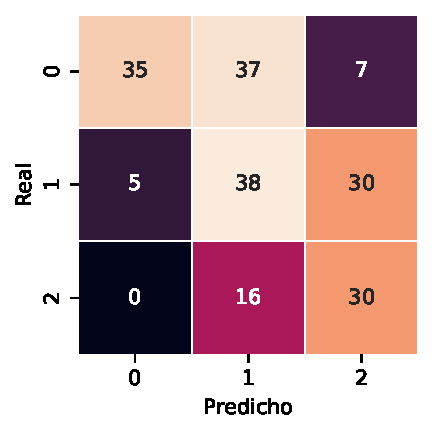
\includegraphics[width=0.6\linewidth]{figures/5_experiments/single-vb-cm.pdf}
    \caption[Característica VB: Matriz de confusión del mejor modelo en datos de test.]{Característica VB: Matriz de confusión del mejor modelo en datos de test. Leyenda: \textbf{0}: Ausente, \textbf{1}: En Formación, \textbf{2}: Presente.}
    \label{fig5:VB_confusion_matrix}
\end{figure}

%% VM
\begin{figure}[htbp]
    \centering
    % --- Top: Table ---
    \begin{minipage}{\linewidth}
        \centering
        \begin{tabular}{c|cc|c|c}
            \hline
            \rowcolor[HTML]{D33333} 
            \multicolumn{1}{|c|}{\cellcolor[HTML]{D33333}{\color[HTML]{FFFFFF} }} & \multicolumn{2}{c|}{\cellcolor[HTML]{D33333}{\color[HTML]{FFFFFF} \textbf{DECR}}} & {\color[HTML]{FFFFFF} \textbf{CONV}} & \multicolumn{1}{c|}{\cellcolor[HTML]{D33333}{\color[HTML]{FFFFFF} \textbf{FN}}} \\ \cline{2-5} 
            \multicolumn{1}{|c|}{\multirow{-2}{*}{\cellcolor[HTML]{D33333}{\color[HTML]{FFFFFF} \textbf{DATA}}}} & \multicolumn{2}{c|}{\cellcolor[HTML]{D33333}{\color[HTML]{FFFFFF} \textbf{GEOD}}} & 256 & \multicolumn{1}{c|}{\textbf{VM}} \\ \cline{1-3} \cline{5-5} 
            \multicolumn{1}{|c|}{\cellcolor[HTML]{D33333}{\color[HTML]{FFFFFF} \textbf{RES}}} & MID & 32 & 256 & \multicolumn{1}{c|}{256} \\ \cline{1-1}
            \multicolumn{1}{|c|}{50K} & OUT & 32 & 16 & \multicolumn{1}{c|}{256} \\ \cline{1-3}
            \multicolumn{1}{|c|}{\cellcolor[HTML]{D33333}{\color[HTML]{FFFFFF} \textbf{TYPE}}} & \multicolumn{2}{c|}{\cellcolor[HTML]{D33333}{\color[HTML]{FFFFFF} \textbf{GEOM}}} & 16 & \multicolumn{1}{c|}{8} \\ \cline{1-3}
            \multicolumn{1}{|c|}{Cut} & MID & 64 & 16 & \multicolumn{1}{c|}{32} \\ \cline{1-1} \cline{5-5} 
             & OUT & 64 & 64 &  \\ \cline{2-4}
        \end{tabular}

        \vspace{1em}
        \begin{tabular}{|
            >{\columncolor[HTML]{D33333}}c |c|c|}
            \hline
            {\color[HTML]{FFFFFF} \textbf{LR}} & $2.4282  \times 10^{-4}$ & \cellcolor[HTML]{D33333}{\color[HTML]{FFFFFF} \textbf{LOSS}} \\ \hline
            {\color[HTML]{FFFFFF} \textbf{OPTIMIZER}} & Adam & \textbf{VM} \\ \hline
            {\color[HTML]{FFFFFF} \textbf{INIT}} & Kaiming & FL \\ \hline
        \end{tabular}
        \captionof{table}{Característica VM: Datos de entrada, estructura de red e hiperparámetros del mejor modelo.}
        \label{table5:VM_best_model}
    \end{minipage}

    \vspace{1.5em} % vertical space between table and image

    % --- Bottom: Figure ---
    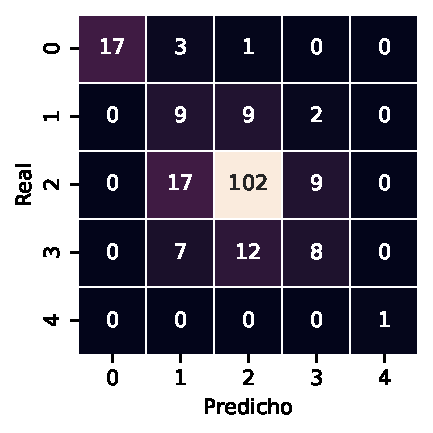
\includegraphics[width=0.6\linewidth]{figures/5_experiments/single-vm-cm.pdf}
    \caption[Característica VM: Matriz de confusión del mejor modelo en datos de test.]{Característica VM: Matriz de confusión del mejor modelo en datos de test. Leyenda: \textbf{0}: Ausente, \textbf{1}: En Formación, \textbf{2}: Formado, Sin Excrecencias, \textbf{3}: Formado, Pocas Excrecencias, \textbf{4}: Formado, Muchas Excrecencias.}
    \label{fig5:VM_confusion_matrix}
\end{figure}

\FloatBarrier

\subsection{Visualización de áreas de interés con Grad-CAM}

Se empleó el método Grad-CAM para visualizar las regiones de las mallas en las que se enfocan los modelos al realizar sus predicciones. En la Figura \ref{fig5:grad_cam__diff_chars} se muestra un ejemplo comparativo entre distintas características, donde puede observarse que cada modelo se centra en una zona distinta de la sínfisis del pubis. Esto refuerza la idea de que los modelos han aprendido patrones morfológicos específicos para cada característica, localizados en distintas áreas del hueso. 

Adicionalmente, se presentan ejemplos individuales de activación de Grad-CAM en las Figuras \ref{fig5:grad_cam__BN_samples}, \ref{fig5:grad_cam__USE_samples} y \ref{fig5:grad_cam__DP_samples}, correspondientes a las características BN, USE y DP, respectivamente. En estos casos, se observa que las zonas de atención se mantienen relativamente consistentes entre distintas muestras, aunque con variaciones según la etiqueta.

En particular, para la característica BN, el modelo concentra su atención en la parte superior de la sínfisis del pubis. Para USE, las activaciones se localizan principalmente en la parte superior izquierda del hueso, con extensiones hacia los laterales y zonas planas de la superficie. Finalmente, para DP, el modelo se enfoca de forma bastante localizada en un solo lateral del hueso.

Estos resultados no solo refuerzan la validez de los modelos entrenados, sino que también aportan evidencia de que las características morfológicas definidas por el método de Todd pueden ser localizadas objetivamente en la superficie del hueso mediante técnicas de DL. Esto representa un paso importante hacia la explicabilidad de modelos aplicados en AF, y abre la puerta a futuras investigaciones colaborativas con expertos humanos para validar y profundizar en estas observaciones para constatar que las regiones anatómicas identificadas son coherentes con la práctica forense.

\begin{figure}[p]
    \centering
    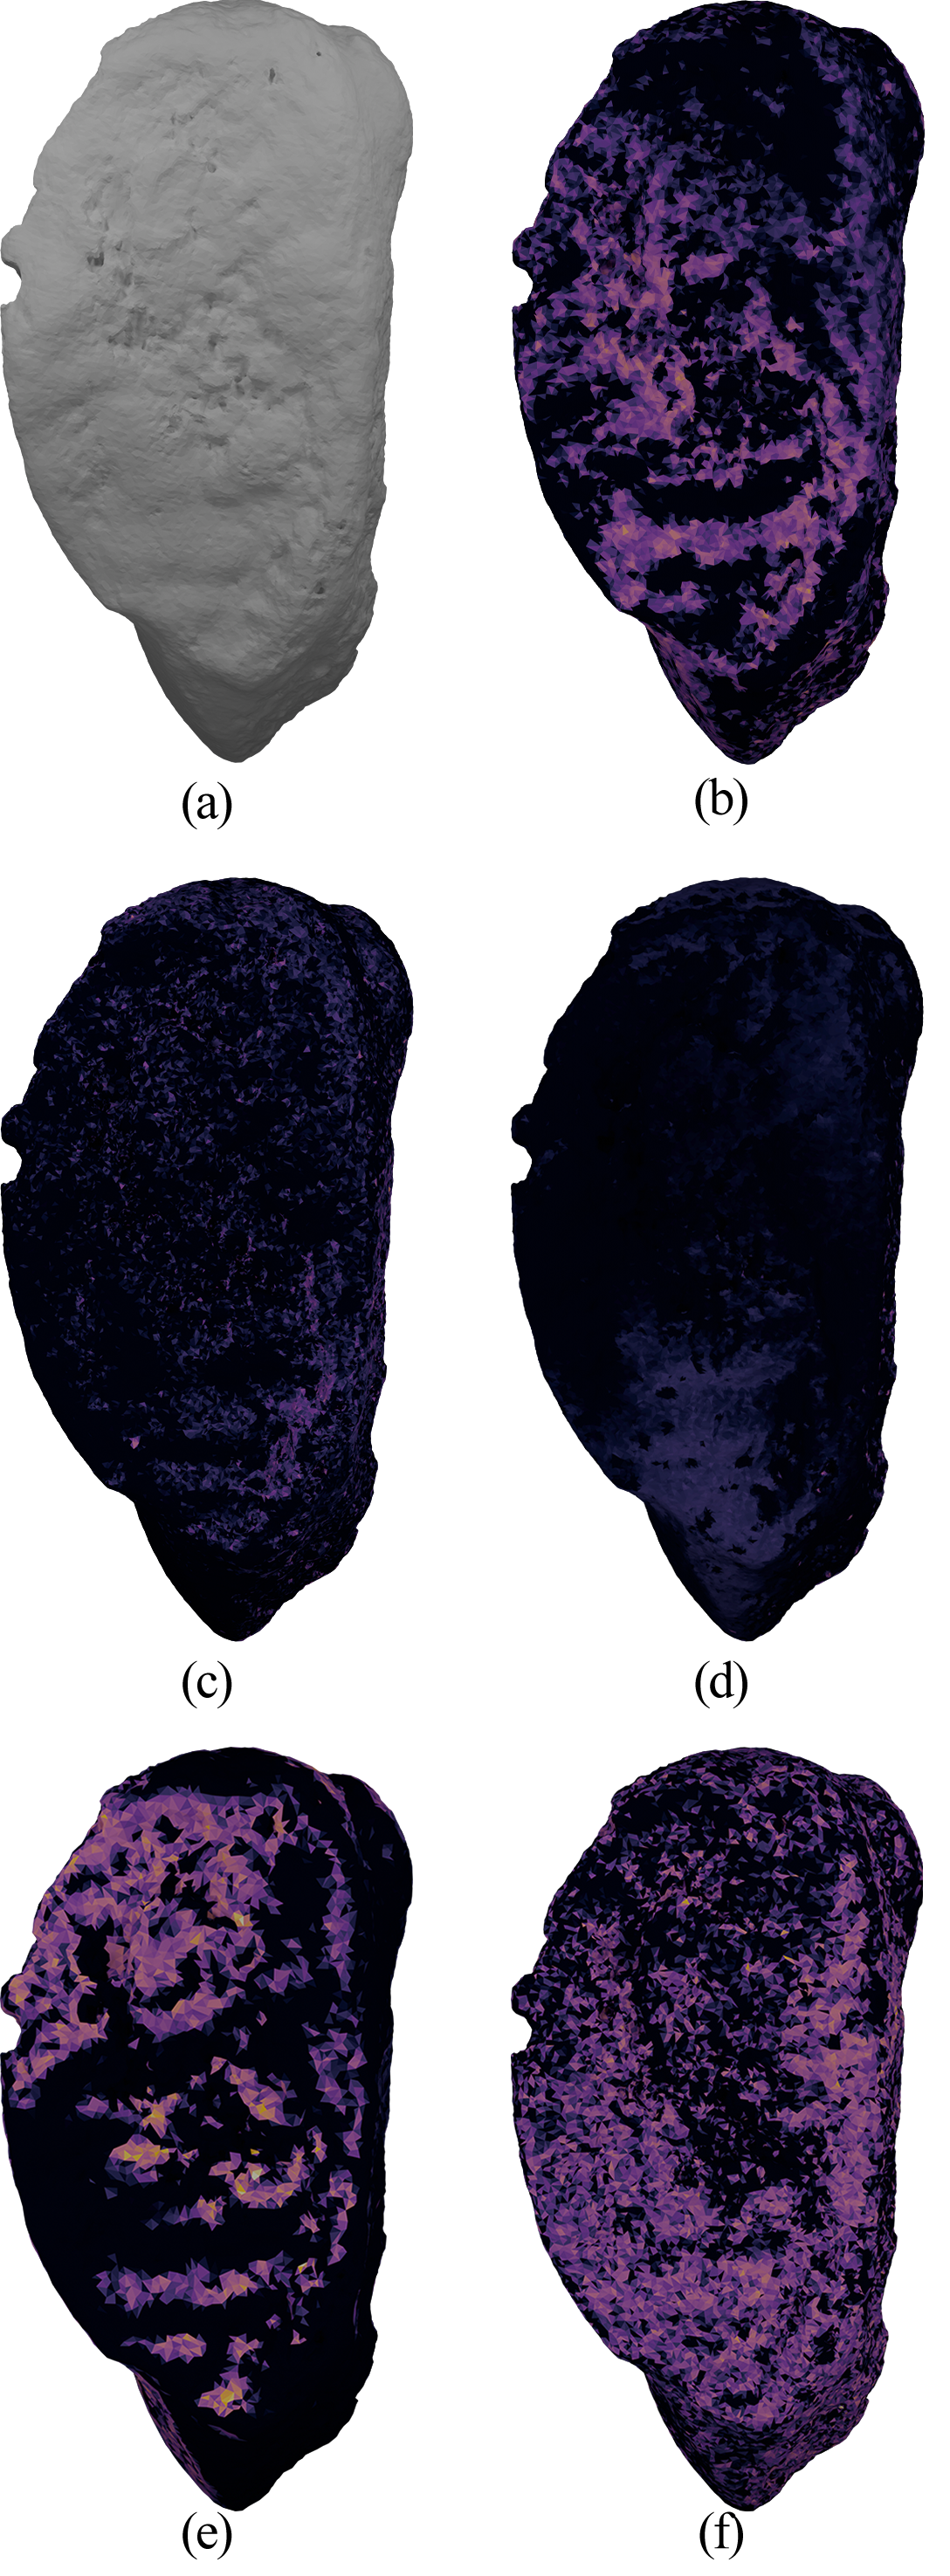
\includegraphics[width=0.5\linewidth]{figures/5_experiments/grad-cam-53-example.png}
    \caption[Ejemplo de mapas de activación de Grad-CAM correspondientes a distintas características para una misma muestra]{Ejemplo de los diferentes mapas de activación de Grad-CAM correspondientes a distintas características para una misma muestra. Los colores más cálidos indican una mayor activación. En (a) se muestra la malla original vista de frente. En este caso se visualizan las características AF (b), DM (c), IP (d), USE (e) y VM (f). Obsérvese cómo cada una se enfoca en regiones diferentes de la malla: algunas con activaciones bien definidas, como (b) y (e); otras con activaciones más dispersas o escasas, como (c) y (d); y (f), con activación en una gran parte de la superficie.}
    \label{fig5:grad_cam__diff_chars}
\end{figure}

\begin{figure}[p]
    \centering
    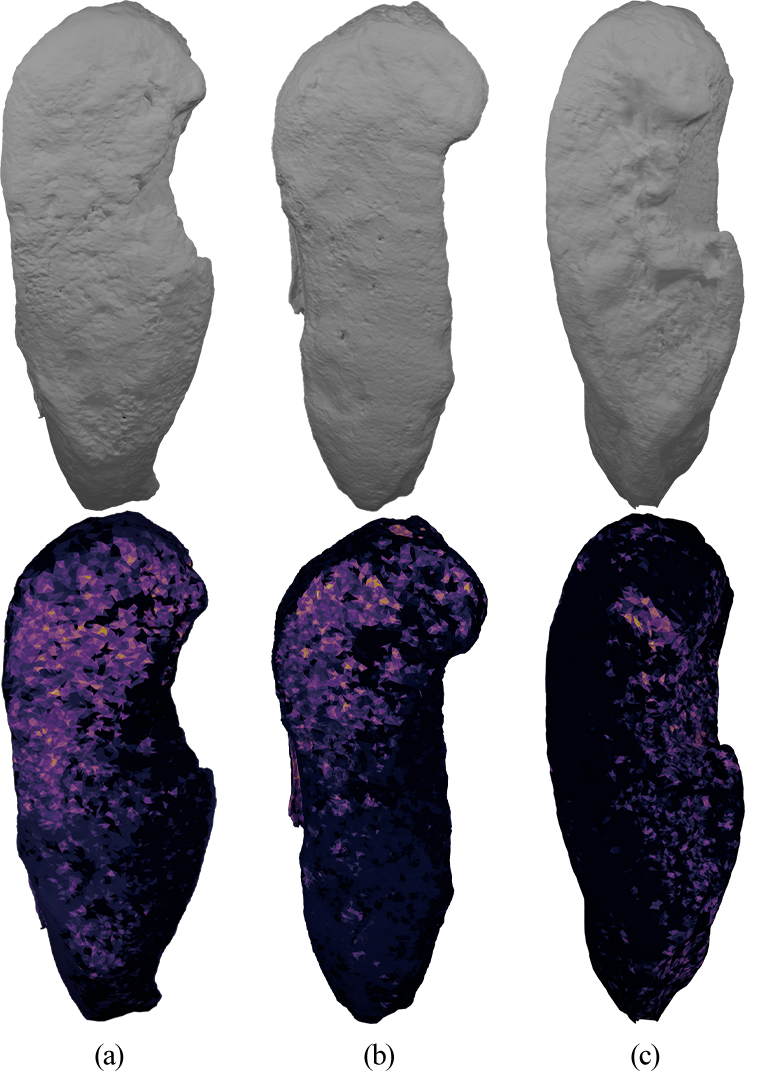
\includegraphics[width=\linewidth]{figures/5_experiments/grad-cam-BN-samples.png}
    \caption[Característica BN: Ejemplo de mapas de activación Grad-CAM]{Característica BN: Ejemplo de mapas de activación Grad-CAM. Se muestran tres mallas diferentes. En la parte superior se presentan las mallas originales, vistas de frente. En la parte inferior, las mismas mallas están coloreadas según la activación de Grad-CAM: los colores más cálidos indican una mayor activación. Se observa que el modelo se enfoca principalmente en la parte superior de la sínfisis del pubis. El modelo ha clasificado correctamente las mallas (a) y (b) como pertenecientes a la clase 0 (\say{ausente}), y la malla (c) a la clase 1 (\say{presente}).}
    \label{fig5:grad_cam__BN_samples}
\end{figure}


\begin{figure}[htbp]
    \centering
    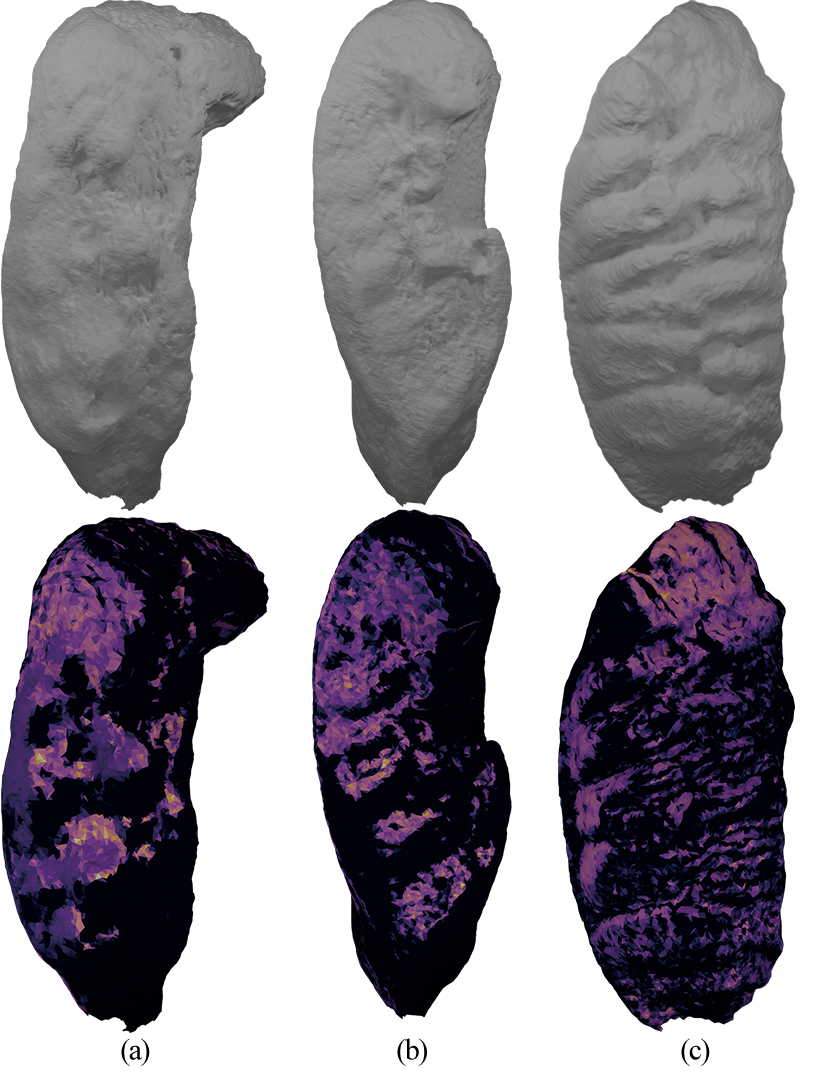
\includegraphics[width=\linewidth]{figures/5_experiments/grad-cam-USE-samples.png}
    \caption[Característica USE: Ejemplo de mapas de activación Grad-CAM]{Característica USE: Ejemplo de mapas de activación Grad-CAM. Se muestran tres mallas diferentes. En la parte superior se presentan las mallas originales, vistas de frente. En la parte inferior, las mismas mallas están coloreadas según la activación de Grad-CAM: los colores más cálidos indican una mayor activación. Se observa que el modelo tiende a enfocarse en la parte superior izquierda del hueso, con activaciones adicionales en los laterales y en zonas planas de la superficie. El modelo ha clasificado correctamente las mallas (a) y (b) como pertenecientes a la clase 1 (\say{definida}) y la malla (c) como 0 (\say{no definida}).}
    \label{fig5:grad_cam__USE_samples}
\end{figure}


\begin{figure}[htbp]
    \centering
    \includegraphics[width=\linewidth]{figures/5_experiments/grad-cam-DP-samples.png}
    \caption[Característica DP: Ejemplo de mapas de activación Grad-CAM]{Característica DP: Ejemplo de mapas de activación Grad-CAM. Se muestran tres mallas diferentes. En la parte superior se presentan las mallas originales, vistas de frente. En la parte inferior, las mismas mallas están coloreadas según la activación de Grad-CAM por triángulo: los colores más cálidos indican mayor activación. Se observa que el modelo se enfoca únicamente en un lateral del hueso. El modelo ha clasificado correctamente las mallas (a) y (c) como pertenecientes a la clase 0 (\say{ausente}), y la malla (b) como 1 (\say{presente}).}
    \label{fig5:grad_cam__DP_samples}
\end{figure}
    
   %  % Conclusiones
    \chapter{Conclusiones y Trabajos Futuros}

La estimación de la edad de la muerte constituye una parte esencial del PB y, al mismo tiempo, un problema complejo de gran relevancia para la AF, debido a la subjetividad inherente a los métodos manuales actualmente empleados por los expertos. Este TFM abordó la clasificación automática de los criterios morfológicos utilizados para dicha estimación por medio de la sínfisis del pubis, con el objetivo de obtener modelos capaces de automatizar la extracción de estos criterios y asistir al experto humano en la toma de decisiones.

En primera instancia, se llevó a cabo un estudio detallado de la literatura sobre estimación de edad a partir de restos óseos, con foco en la sínfisis del pubis, así como del procesamiento de modelos 3D mediante DL. Se observó que la AF continúa utilizando mayoritariamente el método de Todd \cite{RefWorks:RefID:19-todd1921age} o variantes del mismo, con escasa incorporación de innovaciones tecnológicas basadas en DL. En cuanto al tratamiento de datos tridimensionales, se constató la falta de consenso sobre su representación más adecuada, existiendo múltiples alternativas. Para este trabajo se optó por el uso de mallas poligonales, por tratarse de un formato ampliamente utilizado tanto en informática gráfica como en el trabajo cotidiano de los antropólogos forenses. A su vez, no se hallaron estudios previos que aborden la clasificación directa y automática de las características morfológicas del pubis como los aquí planteados.

Se exploraron diversas propuestas metodológicas basadas en mallas poligonales, una representación relativamente novedosa en este campo, y se seleccionó el enfoque ExMeshCNN como \textit{framework} base para el diseño de los modelos, aplicando NAS mediante la librería Optuna \cite{optuna_2019} para optimizar su estructura y demás hiperparámetros relevantes.

El desarrollo de modelos implicó la creación de herramientas específicas para el preprocesamiento de los datos, principalmente la reducción de complejidad topológica mediante colapso de aristas, procurando minimizar la pérdida de información, así como el sellado automático de las mallas. Como parte de los experimentos, se llevaron a cabo 83 ejecuciones que incluyeron un total de 10,800 entrenamientos de modelos entrenados en una etiqueta y 6,000 entrenamientos con múltiples etiquetas por modelo, sumando 16,800 entrenamientos en total. Se obtuvieron así los 9 mejores modelos para cada una de las características del método de Todd, todos con puntuaciones de F1 Macro superiores a 0.6, alcanzando un F1 Macro promedio de 0.6891 y superando el 0.7 en 4 de las 9 características, con una característica obteniendo un valor de 0.92. Cabe destacar que esta métrica (F1 Macro) es conservadora, y el análisis de las matrices de confusión evidencia que los modelos son capaces de clasificar correctamente la mayoría de las muestras, incluso considerando la limitada cantidad de datos y el desbalance entre clases. De igual modo, se obtuvieron valores de igual forma excelentes de \textit{accuracy}, con todos los modelos obteniendo valores superior a 0.5, 4 de las 9 características teniendo valores sobre el 0.9 y un en promedio un valor de \textit{accuracy} de 0.80. Cabe resaltar que, en adición a estos resultados, este TFM es el primer trabajo que se conoce que ha utilizado ExMeshCNN para resolver un problema del mundo real haciendo uso de datos mucho más complejos y con mayor resolución de los que se utilizaron en la publicación original del \textit{framework}.

Asimismo, se empleó Grad-CAM para interpretar las regiones de la malla que influyeron en las predicciones de los modelos. Los resultados muestran que cada modelo se enfoca en zonas distintas del hueso, lo que sugiere que cada característica posee un patrón morfológico diferenciado. En la mayoría de los casos, las regiones de atención se concentraron en la cara anterior del pubis, lo cual coincide con la práctica común de los expertos, validando así que los criterios morfológicos de Todd corresponden efectivamente a patrones estructurales reales. Esto refuerza la idea de que la subjetividad del método de Todd puede mitigarse mediante su automatización. Otro punto interesante que añade peso a esta idea es que se encontraron similitudes entre las características que resultaron más sencillas y más complicadas de detectar por los modelos generados por ExMeshCNN y los forenses, naturalmente esta línea debe ser estudiada en mayor profundidad para obtener conclusiones avaladas por un análisis más detallado, pero resulta un indicio prometedor.

En conclusión, se han alcanzado satisfactoriamente los objetivos planteados, logrando entrenar un modelo por cada una de las características del método de Todd. Todo el código desarrollado se encuentra disponible públicamente en el repositorio de GitHub \url{https://github.com/RhinoBlindado/datcom-tfm}, a excepción del conjunto de datos empleado, cuya distribución está restringida por motivos de confidencialidad.

En definitiva, el trabajo desarrollado sienta una base sólida para futuras líneas de investigación multidisciplinares entre la AF y la IA. Las posibilidades de extensión son amplias: desde la incorporación de técnicas más sofisticadas de NAS, clasificación multietiqueta o regularización, hasta el aumento de la expresividad de los modelos mediante arquitecturas más profundas, mayor número de épocas o la integración de múltiples modelos especializados. La inclusión de información adicional, como las texturas óseas presentes en los escaneos 3D, también podría enriquecer notablemente el proceso de aprendizaje. Finalmente, una colaboración estrecha con expertos forenses permitiría no solo validar las interpretaciones generadas por técnicas como Grad-CAM, sino también identificar nuevas regiones morfológicas relevantes, reforzando así tanto la aplicabilidad práctica como el valor científico del enfoque propuesto.

    % Bibliografía
    \chapter{Bibliografía}
    \printbibliography[heading=none]
    
    % Apéndice
   \appendix
\chapter{Arquitectura e hiperparámetros de los mejores modelos}
\label{best_model_arch}
Para facilitar la comprensión, se incluye una tabla resumen que detalla los datos de entrada utilizados por cada modelo, diferenciando la arquitectura y los otros hiperparámetros seleccionados. La Tabla \ref{table5:sample_table} muestra un ejemplo del formato empleado, junto con la explicación de cada una de sus columnas y filas.

Los mejores modelos obtenidos presentan configuraciones arquitectónicas notablemente diversas entre sí, lo que indica que la búsqueda automática ha sido efectiva para adaptar la estructura de las redes a los requerimientos específicos de cada característica. Pese a esta diversidad, se observa una tendencia general hacia redes con mayor profundidad en las capas convolucionales, como en los casos de AF (Tabla \ref{table5:AF_best_model}), BN (Tabla \ref{table5:BN_best_model}), IP (Tabla \ref{table5:IP_best_model}), LSE (Tabla \ref{table5:LSE_best_model}), VB (Tabla \ref{table5:VB_best_model}) y VM (Tabla \ref{table5:VM_best_model}), donde se utilizaron 4 o más capas convolucionales, y algunas, como AF, BN y VM, alcanzaron hasta 6 capas. Esto sugiere que estas características pueden requerir una mayor capacidad de representación para capturar los patrones complejos presentes en las mallas.

En cuanto al número de filtros por capa, se aprecia un patrón común de expansión y contracción a lo largo de la red, posiblemente reflejando una estructura tipo cuello de botella. USE (Tabla \ref{table5:USE_best_model}) junto con DM y DP (Tabla \ref{table5:DM_DP_best_model}) son las excepciones donde este patrón no se manifiesta claramente. Las capas totalmente conectadas, en cambio, presentan mayor variabilidad en cuanto al número de neuronas y estructura, sin un patrón claro, lo que indica una fuerte dependencia del diseño respecto a la tarea específica.

En términos de hiperparámetros ajenos a la estructura, se detecta un uso consistente del optimizador Adam y de la inicialización Kaiming en la mayoría de los modelos exitosos, lo que sugiere que estas configuraciones son adecuadas para el entrenamiento de redes basadas en ExMeshCNN. En cuanto a las funciones de pérdida, predomina el uso de WCE, seguida por CBL, lo cual es coherente con la naturaleza desbalanceada del problema y valida su idoneidad para este tipo de clasificación. Por parte del \textit{Learning Rate}, se observa que es otra variable muy dependiente de la característica, pero es notable que los valores rondan $1\times10^{-3}$ y $1\times10^{-4}$ los cuales son rangos aceptables para los optimizadores, con LSE siendo la única características cuyo mejor modelo usó valores de $1\times10^{-5}$. 

\begin{figure}[h]
    \begin{minipage}{\linewidth}
        \centering
        \begin{tabular}{c|cc|c|c|}
            \hline
            \rowcolor[HTML]{D33333} 
            \multicolumn{1}{|c|}{\cellcolor[HTML]{D33333}{\color[HTML]{FFFFFF} }} & \multicolumn{2}{c|}{\cellcolor[HTML]{D33333}{\color[HTML]{FFFFFF} \textbf{DECR}}} & {\color[HTML]{FFFFFF} \textbf{CONV}} & {\color[HTML]{FFFFFF} \textbf{FN}} \\ \cline{2-5} 
            \multicolumn{1}{|c|}{\multirow{-2}{*}{\cellcolor[HTML]{D33333}{\color[HTML]{FFFFFF} \textbf{DATA}}}} & \multicolumn{2}{c|}{\cellcolor[HTML]{D33333}{\color[HTML]{FFFFFF} \textbf{GEOD}}} &  & \textbf{(h)} \\ \cline{1-3} \cline{5-5} 
            \multicolumn{1}{|c|}{\cellcolor[HTML]{D33333}{\color[HTML]{FFFFFF} \textbf{RES}}} & MID & (c) &  &  \\ \cline{1-1}
            \multicolumn{1}{|c|}{(a)} & OUT & (d) &  &  \\ \cline{1-3}
            \multicolumn{1}{|c|}{\cellcolor[HTML]{D33333}{\color[HTML]{FFFFFF} \textbf{TYPE}}} & \multicolumn{2}{c|}{\cellcolor[HTML]{D33333}{\color[HTML]{FFFFFF} \textbf{GEOM}}} &  &  \\ \cline{1-3}
            \multicolumn{1}{|c|}{(b)} & MID & (e) &  &  \\ \cline{1-1}
             & OUT & (f) & \multirow{-6}{*}{(g)} & \multirow{-5}{*}{(i)} \\ \cline{2-5} 
        \end{tabular}
    
        \vspace{1em}
    
        \begin{tabular}{|
            >{\columncolor[HTML]{D33333}}c |c|c|}
            \hline
            {\color[HTML]{FFFFFF} \textbf{LR}} & (j) & \cellcolor[HTML]{D33333}{\color[HTML]{FFFFFF} \textbf{LOSS}} \\ \hline
            {\color[HTML]{FFFFFF} \textbf{OPTIMIZER}} & (k) & \textbf{(h)} \\ \hline
            {\color[HTML]{FFFFFF} \textbf{INIT}} & (l) & (n) \\ \hline
        \end{tabular}
        \captionof{table}[Formato de tabla usado para resumir los datos de entrada, la estructura de la red y los hiperparámetros de los mejores modelos]{Formato utilizado para resumir los datos de entrada, la estructura de la red y los hiperparámetros empleados en cada uno de los modelos. La tabla superior detalla las configuraciones relativas a los datos y la arquitectura, mientras que la tabla inferior resume los hiperparámetros principales. En la tabla superior, la columna \textbf{DATA} especifica las características de los datos de entrada: \textbf{RES} indica la resolución de la malla (a) y \textbf{TYPE} su tipo (b). La columna \textbf{DECR} incluye la configuración de los descriptores utilizados: \textbf{GEOD} para el descriptor geodésico y \textbf{GEOM} para el descriptor geométrico; MID y OUT indican respectivamente la densidad de sus capas intermedias (c, e) y de salida (d, f). La columna \textbf{CONV} muestra la arquitectura de las capas convolucionales: número de capas y densidad de cada una (g). La columna \textbf{FN} presenta en (h) las características morfológicas predichas y en (i) la configuración de la parte densa del modelo de cada una. En la tabla inferior, \textbf{LR} indica la tasa de aprendizaje (j), \textbf{OPTIMIZER} el optimizador empleado (k), \textbf{INIT} el tipo de inicialización de pesos (l), y \textbf{LOSS} la función de pérdida (n) asociada a la característica correspondiente (h).}
        \label{table5:sample_table}
    \end{minipage}
\end{figure}

%% AF
\begin{figure}[htbp]
    \centering
    % --- Top: Table ---
    \begin{minipage}{\linewidth}
        \centering
        \begin{tabular}{c|cc|c|cccc|}
            \hline
            \rowcolor[HTML]{D33333} 
            \multicolumn{1}{|c|}{\cellcolor[HTML]{D33333}{\color[HTML]{FFFFFF} }} & \multicolumn{2}{c|}{\cellcolor[HTML]{D33333}{\color[HTML]{FFFFFF} \textbf{DECR}}} & {\color[HTML]{FFFFFF} \textbf{CONV}} & \multicolumn{4}{c|}{\cellcolor[HTML]{D33333}{\color[HTML]{FFFFFF} \textbf{FN}}} \\ \cline{2-8} 
            \multicolumn{1}{|c|}{\multirow{-2}{*}{\cellcolor[HTML]{D33333}{\color[HTML]{FFFFFF} \textbf{DATA}}}} & \multicolumn{2}{c|}{\cellcolor[HTML]{D33333}{\color[HTML]{FFFFFF} \textbf{GEOD}}} & 64 & \multicolumn{1}{c|}{\textbf{AF}} & \multicolumn{1}{c|}{\textbf{DM}} & \multicolumn{1}{c|}{\textbf{LSE}} & \textbf{USE} \\ \cline{1-3} \cline{5-8} 
            \multicolumn{1}{|c|}{\cellcolor[HTML]{D33333}{\color[HTML]{FFFFFF} \textbf{RES}}} & MID & 16 & 32 & \multicolumn{1}{c|}{256} & \multicolumn{1}{c|}{8} & \multicolumn{1}{c|}{16} & 32 \\ \cline{1-1} \cline{5-6}
            \multicolumn{1}{|c|}{50K} & OUT & 128 & 32 &  & \multicolumn{1}{c|}{} & \multicolumn{1}{c|}{8} & 32 \\ \cline{1-3}
            \multicolumn{1}{|c|}{\cellcolor[HTML]{D33333}{\color[HTML]{FFFFFF} \textbf{TYPE}}} & \multicolumn{2}{c|}{\cellcolor[HTML]{D33333}{\color[HTML]{FFFFFF} \textbf{GEOM}}} & 128 &  & \multicolumn{1}{c|}{} & \multicolumn{1}{c|}{64} & 256 \\ \cline{1-3}
            \multicolumn{1}{|c|}{\textit{Cut}} & MID & 128 & 256 &  & \multicolumn{1}{c|}{} & \multicolumn{1}{c|}{128} & 64 \\ \cline{1-1} \cline{7-7}
             & OUT & 256 & 32 &  &  & \multicolumn{1}{c|}{} & 16 \\ \cline{2-4} \cline{8-8} 
        \end{tabular}

        \vspace{1em}

        \begin{tabular}{|
            >{\columncolor[HTML]{D33333}}c |c|
            >{\columncolor[HTML]{FFCCC9}}c ccc|}
            \hline
            {\color[HTML]{FFFFFF} \textbf{LR}} & $3.4261 \times 10^{-4}$ & \multicolumn{4}{c|}{\cellcolor[HTML]{D33333}{\color[HTML]{FFFFFF} \textbf{LOSS}}} \\ \hline
            {\color[HTML]{FFFFFF} \textbf{OPTIMIZER}} & AdamW & \multicolumn{1}{c|}{\textbf{AF}} & \multicolumn{1}{c|}{\textbf{DM}} & \multicolumn{1}{c|}{\textbf{LSE}} & \textbf{USE} \\ \hline
            {\color[HTML]{FFFFFF} \textbf{INIT}} & Uniforme & \multicolumn{1}{c|}{WCE} & \multicolumn{1}{c|}{WCE} & \multicolumn{1}{c|}{CE} & WCE \\ \hline
        \end{tabular}
        \captionof{table}[Característica AF: Datos de entrada, estructura de red e hiperparámetros del mejor modelo.]{Característica \textbf{AF}: Configuración de los datos de entrada, arquitectura de red y otros hiperparámetros del mejor modelo. El mejor modelo hace uso de mallas recortadas (\textit{Cut}) a 50K triángulos de resolución, estructura multietiqueta con AF y sus tres características más asociadas con capas densas variables entre sí. Véase \ref{table5:sample_table} para una descripción de cada elemento de la tabla. Funciones de pérdida: CE: \textit{Cross-Entropy}; WCE: \textit{Weighted Cross-Entropy}.}
        \label{table5:AF_best_model}
    \end{minipage}
\end{figure}

%% BN
\begin{figure}[htbp]
    \centering
    % --- Top: Table ---
    \begin{minipage}{\linewidth}
        \centering
        \begin{tabular}{c|cc|c|cccc}
            \hline
            \rowcolor[HTML]{D33333} 
            \multicolumn{1}{|c|}{\cellcolor[HTML]{D33333}{\color[HTML]{FFFFFF} }} & \multicolumn{2}{c|}{\cellcolor[HTML]{D33333}{\color[HTML]{FFFFFF} \textbf{DECR}}} & {\color[HTML]{FFFFFF} \textbf{CONV}} & \multicolumn{4}{c|}{\cellcolor[HTML]{D33333}{\color[HTML]{FFFFFF} \textbf{FN}}} \\ \cline{2-8} 
            \multicolumn{1}{|c|}{\multirow{-2}{*}{\cellcolor[HTML]{D33333}{\color[HTML]{FFFFFF} \textbf{DATA}}}} & \multicolumn{2}{c|}{\cellcolor[HTML]{D33333}{\color[HTML]{FFFFFF} \textbf{GEOD}}} & 256 & \multicolumn{1}{c|}{\cellcolor[HTML]{FFFFFF}\textbf{AF}} & \multicolumn{1}{c|}{\textbf{BN}} & \multicolumn{1}{c|}{\textbf{DP}} & \multicolumn{1}{c|}{\textbf{LSE}} \\ \cline{1-3} \cline{5-8} 
            \multicolumn{1}{|c|}{\cellcolor[HTML]{D33333}{\color[HTML]{FFFFFF} \textbf{RES}}} & MID & 256 & 128 & \multicolumn{1}{c|}{\cellcolor[HTML]{FFFFFF}128} & \multicolumn{1}{c|}{32} & \multicolumn{1}{c|}{32} & \multicolumn{1}{c|}{32} \\ \cline{1-1} \cline{5-5}
            \multicolumn{1}{|c|}{25K} & OUT & 16 & 256 & \multicolumn{1}{c|}{} & \multicolumn{1}{c|}{64} & \multicolumn{1}{c|}{64} & \multicolumn{1}{c|}{128} \\ \cline{1-3} \cline{6-6}
            \multicolumn{1}{|c|}{\cellcolor[HTML]{D33333}{\color[HTML]{FFFFFF} \textbf{TYPE}}} & \multicolumn{2}{c|}{\cellcolor[HTML]{D33333}{\color[HTML]{FFFFFF} \textbf{GEOM}}} & 64 &  & \multicolumn{1}{c|}{} & \multicolumn{1}{c|}{256} & \multicolumn{1}{c|}{128} \\ \cline{1-3} \cline{8-8} 
            \multicolumn{1}{|c|}{\textit{Cut}} & MID & 32 & 16 &  & \multicolumn{1}{c|}{} & \multicolumn{1}{c|}{16} &  \\ \cline{1-1}
             & OUT & 16 & 64 &  & \multicolumn{1}{c|}{} & \multicolumn{1}{c|}{256} &  \\ \cline{2-4} \cline{7-7}
        \end{tabular}

        \vspace{1em}

        \begin{tabular}{|
            >{\columncolor[HTML]{D33333}}c |c|c
            >{\columncolor[HTML]{FFCCC9}}c cc|}
            \hline
            {\color[HTML]{FFFFFF} \textbf{LR}} & $5.0965 \times 10^{-3}$ & \multicolumn{4}{c|}{\cellcolor[HTML]{D33333}{\color[HTML]{FFFFFF} \textbf{LOSS}}} \\ \hline
            {\color[HTML]{FFFFFF} \textbf{OPTIMIZER}} & Radam & \multicolumn{1}{c|}{\textbf{AF}} & \multicolumn{1}{c|}{\textbf{BN}} & \multicolumn{1}{c|}{\textbf{DP}} & \textbf{LSE} \\ \hline
            {\color[HTML]{FFFFFF} \textbf{INIT}} & Kaiming & \multicolumn{1}{c|}{FL} & \multicolumn{1}{c|}{CBL} & \multicolumn{1}{c|}{CBL} & CBL \\ \hline
        \end{tabular}
        \captionof{table}[Característica BN: Datos de entrada, estructura de red e hiperparámetros del mejor modelo.]{Característica \textbf{BN}: Configuración de los datos de entrada, arquitectura de red y otros hiperparámetros del mejor modelo. El mejor modelo hace uso de mallas recortadas (\textit{Cut}) a 25K triángulos de resolución, estructura multietiqueta con BN y sus tres características más asociadas con capas densas variables entre sí. Véase \ref{table5:sample_table} para una descripción de cada elemento de la tabla. Funciones de pérdida: FL: \textit{Focal Loss}; CBL: \textit{Class-Balanced Loss}.}
        \label{table5:BN_best_model}
    \end{minipage}
\end{figure}

%% DM / DP
\begin{figure}[htbp]
    \centering
    % --- Top: Table ---
    \begin{minipage}{\linewidth}
        \centering
        \begin{tabular}{c|cc|cc}
            \hline
            \rowcolor[HTML]{D33333} 
            \multicolumn{1}{|c|}{\cellcolor[HTML]{D33333}{\color[HTML]{FFFFFF} }} & \multicolumn{2}{c|}{\cellcolor[HTML]{D33333}{\color[HTML]{FFFFFF} \textbf{DECR}}} & \multicolumn{1}{c|}{\cellcolor[HTML]{D33333}{\color[HTML]{FFFFFF} \textbf{CONV}}} & \multicolumn{1}{c|}{\cellcolor[HTML]{D33333}{\color[HTML]{FFFFFF} \textbf{FN}}} \\ \cline{2-5} 
            \multicolumn{1}{|c|}{\multirow{-2}{*}{\cellcolor[HTML]{D33333}{\color[HTML]{FFFFFF} \textbf{DATA}}}} & \multicolumn{2}{c|}{\cellcolor[HTML]{D33333}{\color[HTML]{FFFFFF} \textbf{GEOD}}} & \multicolumn{1}{c|}{64} & \multicolumn{1}{c|}{\textbf{Todos}} \\ \cline{1-3} \cline{5-5} 
            \multicolumn{1}{|c|}{\cellcolor[HTML]{D33333}{\color[HTML]{FFFFFF} \textbf{RES}}} & MID & 16 & \multicolumn{1}{c|}{128} & \multicolumn{1}{c|}{32} \\ \cline{1-1} \cline{5-5} 
            \multicolumn{1}{|c|}{100K} & OUT & 16 & \multicolumn{1}{c|}{128} &  \\ \cline{1-4}
            \multicolumn{1}{|c|}{\cellcolor[HTML]{D33333}{\color[HTML]{FFFFFF} \textbf{TYPE}}} & \multicolumn{2}{c|}{\cellcolor[HTML]{D33333}{\color[HTML]{FFFFFF} \textbf{GEOM}}} &  &  \\ \cline{1-3}
            \multicolumn{1}{|c|}{\textit{Cut}} & MID & 16 &  &  \\ \cline{1-1}
             & OUT & 256 &  &  \\ \cline{2-3}
        \end{tabular}

        \vspace{1em}

        \begin{tabular}{cc|ccccc}
        \hline
        \multicolumn{1}{|c|}{\cellcolor[HTML]{D33333}{\color[HTML]{FFFFFF} \textbf{LR}}} & $1.4861 \times 10^{-4}$ & \multicolumn{5}{c|}{\cellcolor[HTML]{D33333}{\color[HTML]{FFFFFF} \textbf{LOSS}}} \\ \hline
        \multicolumn{1}{|c|}{\cellcolor[HTML]{D33333}{\color[HTML]{FFFFFF} \textbf{OPTIMIZER}}} & Adam & \multicolumn{1}{c|}{\textbf{AF}} & \multicolumn{1}{c|}{\textbf{BN}} & \multicolumn{1}{c|}{\textbf{DM}} & \multicolumn{1}{c|}{\textbf{DP}} & \multicolumn{1}{c|}{\textbf{IP}} \\ \hline
        \multicolumn{1}{|c|}{\cellcolor[HTML]{D33333}{\color[HTML]{FFFFFF} \textbf{INIT}}} & Kaiming & \multicolumn{1}{c|}{WCE} & \multicolumn{1}{c|}{CE} & \multicolumn{1}{c|}{CE} & \multicolumn{1}{c|}{CE} & \multicolumn{1}{c|}{WCE} \\ \hline
        &  & \multicolumn{1}{c|}{\textbf{LSE}} & \multicolumn{1}{c|}{\textbf{USE}} & \multicolumn{1}{c|}{\textbf{VB}} & \multicolumn{1}{c|}{\textbf{VM}} &  \\ \cline{3-6}
        &  & \multicolumn{1}{c|}{CE} & \multicolumn{1}{c|}{WCE} & \multicolumn{1}{c|}{CE} & \multicolumn{1}{c|}{CE} &  \\ \cline{3-6}
        \end{tabular}
        \captionof{table}[Característica DM y DP: Datos de entrada, estructura de red e hiperparámetros del mejor modelo.]{Características \textbf{DM} y \textbf{DP}: Configuración de los datos de entrada, arquitectura de red y otros hiperparámetros del mejor modelo. El mejor modelo hace uso de mallas recortadas (\textit{Cut}) a 100K triángulos de resolución, estructura multietiqueta utilizando todas las características con capas densas idénticas entre sí. Véase \ref{table5:sample_table} para una descripción de cada elemento de la tabla. Funciones de pérdida: CE: \textit{Cross-Entropy}; WCE: \textit{Weighted Cross-Entropy}.}
        \label{table5:DM_DP_best_model}
    \end{minipage}
\end{figure}

%% IP
\begin{figure}[htbp]
    \centering
    % --- Top: Table ---
    \begin{minipage}{\linewidth}
        \centering
        \begin{tabular}{c|cc|cc}
            \hline
            \rowcolor[HTML]{D33333} 
            \multicolumn{1}{|c|}{\cellcolor[HTML]{D33333}{\color[HTML]{FFFFFF} }} & \multicolumn{2}{c|}{\cellcolor[HTML]{D33333}{\color[HTML]{FFFFFF} \textbf{DECR}}} & \multicolumn{1}{c|}{\cellcolor[HTML]{D33333}{\color[HTML]{FFFFFF} \textbf{CONV}}} & \multicolumn{1}{c|}{\cellcolor[HTML]{D33333}{\color[HTML]{FFFFFF} \textbf{FN}}} \\ \cline{2-5} 
            \multicolumn{1}{|c|}{\multirow{-2}{*}{\cellcolor[HTML]{D33333}{\color[HTML]{FFFFFF} \textbf{DATA}}}} & \multicolumn{2}{c|}{\cellcolor[HTML]{D33333}{\color[HTML]{FFFFFF} \textbf{GEOD}}} & \multicolumn{1}{c|}{64} & \multicolumn{1}{c|}{\textbf{IP}} \\ \cline{1-3} \cline{5-5} 
            \multicolumn{1}{|c|}{\cellcolor[HTML]{D33333}{\color[HTML]{FFFFFF} \textbf{RES}}} & MID & 256 & \multicolumn{1}{c|}{128} & \multicolumn{1}{c|}{256} \\ \cline{1-1} \cline{5-5} 
            \multicolumn{1}{|c|}{100K} & OUT & 32 & \multicolumn{1}{c|}{64} &  \\ \cline{1-3}
            \multicolumn{1}{|c|}{\cellcolor[HTML]{D33333}{\color[HTML]{FFFFFF} \textbf{TYPE}}} & \multicolumn{2}{c|}{\cellcolor[HTML]{D33333}{\color[HTML]{FFFFFF} \textbf{GEOM}}} & \multicolumn{1}{c|}{64} &  \\ \cline{1-3}
            \multicolumn{1}{|c|}{\textit{Cut}} & MID & 16 & \multicolumn{1}{c|}{32} &  \\ \cline{1-1} \cline{4-4}
             & OUT & 256 &  &  \\ \cline{2-3}
        \end{tabular}

        \vspace{1em}

        \begin{tabular}{|
            >{\columncolor[HTML]{D33333}}c |c|c|}
            \hline
            {\color[HTML]{FFFFFF} \textbf{LR}} & $1.2990 \times 10^{-3}$ & \cellcolor[HTML]{D33333}{\color[HTML]{FFFFFF} \textbf{LOSS}} \\ \hline
            {\color[HTML]{FFFFFF} \textbf{OPTIMIZER}} & Radam & \textbf{IP} \\ \hline
            {\color[HTML]{FFFFFF} \textbf{INIT}} & Kaiming & WCE \\ \hline
        \end{tabular}
        \captionof{table}[Característica IP: Datos de entrada, estructura de red e hiperparámetros del mejor modelo.]{Característica \textbf{IP}: Configuración de los datos de entrada, arquitectura de red y otros hiperparámetros del mejor modelo. El mejor modelo hace uso de mallas recortadas (\textit{Cut}) a 100K triángulos de resolución, estructura de etiqueta única. Véase \ref{table5:sample_table} para una descripción de cada elemento de la tabla. Funciones de pérdida: WCE: \textit{Weighted Cross-Entropy}.}
        \label{table5:IP_best_model}
    \end{minipage}
\end{figure}

%% LSE
\begin{figure}[htbp]
    \centering
    % --- Top: Table ---
    \begin{minipage}{\linewidth}
        \centering
        \begin{tabular}{c|cc|cc}
            \hline
            \rowcolor[HTML]{D33333} 
            \multicolumn{1}{|c|}{\cellcolor[HTML]{D33333}{\color[HTML]{FFFFFF} }} & \multicolumn{2}{c|}{\cellcolor[HTML]{D33333}{\color[HTML]{FFFFFF} \textbf{DECR}}} & \multicolumn{1}{c|}{\cellcolor[HTML]{D33333}{\color[HTML]{FFFFFF} \textbf{CONV}}} & \multicolumn{1}{c|}{\cellcolor[HTML]{D33333}{\color[HTML]{FFFFFF} \textbf{FN}}} \\ \cline{2-5} 
            \multicolumn{1}{|c|}{\multirow{-2}{*}{\cellcolor[HTML]{D33333}{\color[HTML]{FFFFFF} \textbf{DATA}}}} & \multicolumn{2}{c|}{\cellcolor[HTML]{D33333}{\color[HTML]{FFFFFF} \textbf{GEOD}}} & \multicolumn{1}{c|}{256} & \multicolumn{1}{c|}{\textbf{LSE}} \\ \cline{1-3} \cline{5-5} 
            \multicolumn{1}{|c|}{\cellcolor[HTML]{D33333}{\color[HTML]{FFFFFF} \textbf{RES}}} & MID & 32 & \multicolumn{1}{c|}{16} & \multicolumn{1}{c|}{8} \\ \cline{1-1}
            \multicolumn{1}{|c|}{100K} & OUT & 64 & \multicolumn{1}{c|}{64} & \multicolumn{1}{c|}{16} \\ \cline{1-3}
            \multicolumn{1}{|c|}{\cellcolor[HTML]{D33333}{\color[HTML]{FFFFFF} \textbf{TYPE}}} & \multicolumn{2}{c|}{\cellcolor[HTML]{D33333}{\color[HTML]{FFFFFF} \textbf{GEOM}}} & \multicolumn{1}{c|}{16} & \multicolumn{1}{c|}{256} \\ \cline{1-4}
            \multicolumn{1}{|c|}{\textit{Full}} & MID & 256 & \multicolumn{1}{c|}{} & \multicolumn{1}{c|}{128} \\ \cline{1-1} \cline{5-5} 
             & OUT & 128 &  &  \\ \cline{2-3}
    \end{tabular}

        \vspace{1em}

        \begin{tabular}{|
            >{\columncolor[HTML]{D33333}}c |c|c|}
            \hline
            {\color[HTML]{FFFFFF} \textbf{LR}} & $8.4586 \times 10^{-5}$ & \cellcolor[HTML]{D33333}{\color[HTML]{FFFFFF} \textbf{LOSS}} \\ \hline
            {\color[HTML]{FFFFFF} \textbf{OPTIMIZER}} & Adam & \textbf{LSE} \\ \hline
            {\color[HTML]{FFFFFF} \textbf{INIT}} & Orthogonal & WCE \\ \hline
        \end{tabular}
        \captionof{table}[Característica LSE: Datos de entrada, estructura de red e hiperparámetros del mejor modelo.]{Característica \textbf{LSE}: Configuración de los datos de entrada, arquitectura de red y otros hiperparámetros del mejor modelo. El mejor modelo hace uso de mallas completas (\textit{Full}) a 100K triángulos de resolución, estructura de etiqueta única. Véase \ref{table5:sample_table} para una descripción de cada elemento de la tabla. Funciones de pérdida: WCE: \textit{Weighted Cross-Entropy}.}
        \label{table5:LSE_best_model}
    \end{minipage}
\end{figure}

%% USE
\begin{figure}[htbp]
    \centering
    % --- Top: Table ---
    \begin{minipage}{\linewidth}
        \centering
        \begin{tabular}{c|cc|cc}
            \hline
            \rowcolor[HTML]{D33333} 
            \multicolumn{1}{|c|}{\cellcolor[HTML]{D33333}{\color[HTML]{FFFFFF} }} & \multicolumn{2}{c|}{\cellcolor[HTML]{D33333}{\color[HTML]{FFFFFF} \textbf{DECR}}} & \multicolumn{1}{c|}{\cellcolor[HTML]{D33333}{\color[HTML]{FFFFFF} \textbf{CONV}}} & \multicolumn{1}{c|}{\cellcolor[HTML]{D33333}{\color[HTML]{FFFFFF} \textbf{FN}}} \\ \cline{2-5} 
            \multicolumn{1}{|c|}{\multirow{-2}{*}{\cellcolor[HTML]{D33333}{\color[HTML]{FFFFFF} \textbf{DATA}}}} & \multicolumn{2}{c|}{\cellcolor[HTML]{D33333}{\color[HTML]{FFFFFF} \textbf{GEOD}}} & \multicolumn{1}{c|}{32} & \multicolumn{1}{c|}{\textbf{Todos}} \\ \cline{1-3} \cline{5-5} 
            \multicolumn{1}{|c|}{\cellcolor[HTML]{D33333}{\color[HTML]{FFFFFF} \textbf{RES}}} & MID & 128 & \multicolumn{1}{c|}{32} & \multicolumn{1}{c|}{16} \\ \cline{1-1} \cline{4-5} 
            \multicolumn{1}{|c|}{25K} & OUT & 256 &  &  \\ \cline{1-3}
            \multicolumn{1}{|c|}{\cellcolor[HTML]{D33333}{\color[HTML]{FFFFFF} \textbf{TYPE}}} & \multicolumn{2}{c|}{\cellcolor[HTML]{D33333}{\color[HTML]{FFFFFF} \textbf{GEOM}}} &  &  \\ \cline{1-3}
            \multicolumn{1}{|c|}{\textit{Cut}} & MID & 16 &  &  \\ \cline{1-1}
             & OUT & 32 &  &  \\ \cline{2-3}
        \end{tabular}

        \vspace{1em}

        \begin{tabular}{|
            >{\columncolor[HTML]{D33333}}c |c|ccc
            >{\columncolor[HTML]{FFCCC9}}c c|}
            \hline
            {\color[HTML]{FFFFFF} \textbf{LR}} & $1.3456 \times 10^{-3}$ & \multicolumn{5}{c|}{\cellcolor[HTML]{D33333}{\color[HTML]{FFFFFF} \textbf{LOSS}}} \\ \hline
            {\color[HTML]{FFFFFF} \textbf{OPTIMIZER}} & Adam & \multicolumn{1}{c|}{\textbf{AF}} & \multicolumn{1}{c|}{\textbf{DM}} & \multicolumn{1}{c|}{\textbf{LSE}} & \multicolumn{1}{c|}{\textbf{USE}} & \textbf{IP} \\ \hline
            {\color[HTML]{FFFFFF} \textbf{INIT}} & Kaiming & \multicolumn{1}{c|}{CBL} & \multicolumn{1}{c|}{CE} & \multicolumn{1}{c|}{CBL} & \multicolumn{1}{c|}{FL} & WCE \\ \hline
        \end{tabular}
        \captionof{table}[Característica USE: Datos de entrada, estructura de red e hiperparámetros del mejor modelo.]{Característica \textbf{USE}: Configuración de los datos de entrada, arquitectura de red y otros hiperparámetros del mejor modelo. El mejor modelo hace uso de mallas recortadas (\textit{Cut}) a 25K triángulos de resolución, estructura multietiqueta con USE y sus tres características más asociadas con capas densas idénticas entre sí. Véase \ref{table5:sample_table} para una descripción de cada elemento de la tabla. Funciones de pérdida: CE: \textit{Cross-Entropy}; WCE: \textit{Weighted Cross-Entropy}; FL: \textit{Focal Loss}; CBL: \textit{Class-Balanced Loss}.}
        \label{table5:USE_best_model}
    \end{minipage}
\end{figure}

%% VB
\begin{figure}[htbp]
    \centering
    % --- Top: Table ---
    \begin{minipage}{\linewidth}
        \centering
        \begin{tabular}{c|cc|c|c|}
            \hline
            \rowcolor[HTML]{D33333} 
            \multicolumn{1}{|c|}{\cellcolor[HTML]{D33333}{\color[HTML]{FFFFFF} }} & \multicolumn{2}{c|}{\cellcolor[HTML]{D33333}{\color[HTML]{FFFFFF} \textbf{DECR}}} & {\color[HTML]{FFFFFF} \textbf{CONV}} & {\color[HTML]{FFFFFF} \textbf{FN}} \\ \cline{2-5} 
            \multicolumn{1}{|c|}{\multirow{-2}{*}{\cellcolor[HTML]{D33333}{\color[HTML]{FFFFFF} \textbf{DATA}}}} & \multicolumn{2}{c|}{\cellcolor[HTML]{D33333}{\color[HTML]{FFFFFF} \textbf{GEOD}}} & 64 & \textbf{VB} \\ \cline{1-3} \cline{5-5} 
            \multicolumn{1}{|c|}{\cellcolor[HTML]{D33333}{\color[HTML]{FFFFFF} \textbf{RES}}} & MID & 128 & 256 & 8 \\ \cline{1-1}
            \multicolumn{1}{|c|}{50K} & OUT & 256 & 16 & 256 \\ \cline{1-3}
            \multicolumn{1}{|c|}{\cellcolor[HTML]{D33333}{\color[HTML]{FFFFFF} \textbf{TYPE}}} & \multicolumn{2}{c|}{\cellcolor[HTML]{D33333}{\color[HTML]{FFFFFF} \textbf{GEOM}}} & 16 & 8 \\ \cline{1-4}
            \multicolumn{1}{|c|}{\textit{Cut}} & MID & 256 &  & 128 \\ \cline{1-1}
             & OUT & 32 &  & 32 \\ \cline{2-3} \cline{5-5} 
        \end{tabular}

        \vspace{1em}

        \begin{tabular}{|
            >{\columncolor[HTML]{D33333}}c |c|c|}
            \hline
            {\color[HTML]{FFFFFF} \textbf{LR}} & $7.9839  \times 10^{-3}$ & \cellcolor[HTML]{D33333}{\color[HTML]{FFFFFF} \textbf{LOSS}} \\ \hline
            {\color[HTML]{FFFFFF} \textbf{OPTIMIZER}} & Adam & \textbf{VB} \\ \hline
            {\color[HTML]{FFFFFF} \textbf{INIT}} & Kaiming & CE \\ \hline
        \end{tabular}
        \captionof{table}[Característica VB: Datos de entrada, estructura de red e hiperparámetros del mejor modelo.]{Característica \textbf{VB}: Configuración de los datos de entrada, arquitectura de red y otros hiperparámetros del mejor modelo. El mejor modelo hace uso de mallas recortadas (\textit{Cut}) a 50K triángulos de resolución, estructura de etiqueta única. Véase \ref{table5:sample_table} para una descripción de cada elemento de la tabla. Funciones de pérdida: CE: \textit{Cross-Entropy}.}
        \label{table5:VB_best_model}
    \end{minipage}
\end{figure}

%% VM
\begin{figure}[htbp]
    \centering
    % --- Top: Table ---
    \begin{minipage}{\linewidth}
        \centering
        \begin{tabular}{c|cc|c|c}
            \hline
            \rowcolor[HTML]{D33333} 
            \multicolumn{1}{|c|}{\cellcolor[HTML]{D33333}{\color[HTML]{FFFFFF} }} & \multicolumn{2}{c|}{\cellcolor[HTML]{D33333}{\color[HTML]{FFFFFF} \textbf{DECR}}} & {\color[HTML]{FFFFFF} \textbf{CONV}} & \multicolumn{1}{c|}{\cellcolor[HTML]{D33333}{\color[HTML]{FFFFFF} \textbf{FN}}} \\ \cline{2-5} 
            \multicolumn{1}{|c|}{\multirow{-2}{*}{\cellcolor[HTML]{D33333}{\color[HTML]{FFFFFF} \textbf{DATA}}}} & \multicolumn{2}{c|}{\cellcolor[HTML]{D33333}{\color[HTML]{FFFFFF} \textbf{GEOD}}} & 256 & \multicolumn{1}{c|}{\textbf{VM}} \\ \cline{1-3} \cline{5-5} 
            \multicolumn{1}{|c|}{\cellcolor[HTML]{D33333}{\color[HTML]{FFFFFF} \textbf{RES}}} & MID & 32 & 256 & \multicolumn{1}{c|}{256} \\ \cline{1-1}
            \multicolumn{1}{|c|}{50K} & OUT & 32 & 16 & \multicolumn{1}{c|}{256} \\ \cline{1-3}
            \multicolumn{1}{|c|}{\cellcolor[HTML]{D33333}{\color[HTML]{FFFFFF} \textbf{TYPE}}} & \multicolumn{2}{c|}{\cellcolor[HTML]{D33333}{\color[HTML]{FFFFFF} \textbf{GEOM}}} & 16 & \multicolumn{1}{c|}{8} \\ \cline{1-3}
            \multicolumn{1}{|c|}{\textit{Cut}} & MID & 64 & 16 & \multicolumn{1}{c|}{32} \\ \cline{1-1} \cline{5-5} 
             & OUT & 64 & 64 &  \\ \cline{2-4}
        \end{tabular}

        \vspace{1em}
        
        \begin{tabular}{|
            >{\columncolor[HTML]{D33333}}c |c|c|}
            \hline
            {\color[HTML]{FFFFFF} \textbf{LR}} & $2.4282  \times 10^{-4}$ & \cellcolor[HTML]{D33333}{\color[HTML]{FFFFFF} \textbf{LOSS}} \\ \hline
            {\color[HTML]{FFFFFF} \textbf{OPTIMIZER}} & Adam & \textbf{VM} \\ \hline
            {\color[HTML]{FFFFFF} \textbf{INIT}} & Kaiming & FL \\ \hline
        \end{tabular}
        \captionof{table}[Característica VM: Datos de entrada, estructura de red e hiperparámetros del mejor modelo.]{Característica \textbf{VM}: Configuración de los datos de entrada, arquitectura de red y otros hiperparámetros del mejor modelo. El mejor modelo hace uso de mallas recortadas (\textit{Cut}) a 50K triángulos de resolución, estructura de etiqueta única. Véase \ref{table5:sample_table} para una descripción de cada elemento de la tabla. Funciones de pérdida: FL: \textit{Focal Loss}.}
        \label{table5:VM_best_model}
    \end{minipage}
\end{figure}

    \chapter*{}
    \thispagestyle{empty}

%%\nocite{*}
%\appendix
%\input{apendices/manual_usuario/manual_usuario}
%%\input{apendices/paper/paper}
%\input{glosario/entradas_glosario}
% \addcontentsline{toc}{chapter}{Glosario}
% \printglossary



\end{document}
